%% This is file `elsarticle-template-2-harv.tex',
%%
%% Copyright 2009 Elsevier Ltd
%%
%% This file is part of the 'Elsarticle Bundle'.
%% ---------------------------------------------
%%
%% It may be distributed under the conditions of the LaTeX Project Public
%% License, either version 1.2 of this license or (at your option) any
%% later version.  The latest version of this license is in
%%    http://www.latex-project.org/lppl.txt
%% and version 1.2 or later is part of all distributions of LaTeX
%% version 1999/12/01 or later.
%%
%% The list of all files belonging to the 'Elsarticle Bundle' is
%% given in the file `manifest.txt'.
%%
%% Template article for Elsevier's document class `elsarticle'
%% with harvard style bibliographic references
%%
%% $Id: elsarticle-template-2-harv.tex 155 2009-10-08 05:35:05Z rishi $
%% $URL: http://lenova.river-valley.com/svn/elsbst/trunk/elsarticle-template-2-harv.tex $
%%
\documentclass[review,authoryear,12pt]{elsarticle}
% \documentclass[draft,authoryear,12pt]{elsarticle}
%
%% Use the option review to obtain double line spacing
 % \documentclass[authoryear,preprint,review,12pt]{elsarticle}

%% Use the options 1p,twocolumn; 3p; 3p,twocolumn; 5p; or 5p,twocolumn
%% for a journal layout:
% \documentclass[final,authoryear,1p,times]{elsarticle}
% \documentclass[final,authoryear,1p,times,twocolumn]{elsarticle}
% \documentclass[final,authoryear,3p,times]{elsarticle}
 % \documentclass[final,authoryear,3p,times,twocolumn]{elsarticle}
% \documentclass[final,authoryear,5p,times]{elsarticle}
% \documentclass[final,authoryear,5p,times,twocolumn]{elsarticle}

%% if you use PostScript figures in your article
%% use the graphics package for simple commands
%% \usepackage{graphics}
%% or use the graphicx package for more complicated commands
%% \usepackage{graphicx}
%% or use the epsfig package if you prefer to use the old commands
%% \usepackage{epsfig}
%
\usepackage{amssymb} % The amssymb package provides various useful mathematical symbols
\usepackage{graphicx} % Required for the inclusion of images
\usepackage{placeins} % for float barrier - stops figures from moving
\usepackage{adjustbox} % for resizing tables.
\usepackage[version=4]{mhchem} % Package for chemical equation typesetting
%\usepackage{fontspec} % allows insertion of special characters such as \UTF{00C3}\UTF{0083}\UTF{017E} and \UTF{00C3}\UTF{0083}\UTF{00A9}%
\usepackage{siunitx}
\usepackage{rotating}
\usepackage{pdflscape}
\usepackage{booktabs}
%\usepackage[CaptionAfterwards]{fltpage} % for caption on following page to figure.


%%% Remove the next two lines if you want the figures at their place    
\usepackage[nomarkers,figuresonly]{endfloat}
\renewcommand{\processdelayedfloats}{}

\usepackage[printfigures]{figcaps} % printfigures to display figure floats
\figcapsoff % enable to keep floats in their positions 

% The amsthm package provides extended theorem environments
% \usepackage{amsthm}
 
% The lineno packages adds line numbers. Start line numbering with
% \begin{linenumbers}, end it with \end{linenumbers}. Or switch it on
%% for the whole article with \linenumbers after \end{frontmatter}.
 \usepackage{lineno}
 
 %Supplementary figures and tables
 \newcommand{\beginsupplement}{%
        \setcounter{table}{0}
        \renewcommand{\thetable}{S\arabic{table}}%
        \setcounter{figure}{0}
        \renewcommand{\thefigure}{S\arabic{figure}}%
     } 
 
\newcommand{\dgC}{$^\circ$C }
\newcommand{\dgCs}{$^\circ$C}
\newcommand{\fO}{\textit{f}O$_{2}$ }

% natbib.sty is loaded by default. However, natbib options can be
% provided with \biboptions{...} command. Following options are
% valid:

%   round  -  round parentheses are used (default)
%   square -  square brackets are used   [option]
%   curly  -  curly braces are used      {option}
%   angle  -  angle brackets are used    <option>
%   semicolon  -  multiple citations separated by semi-colon (default)
%   colon  - same as semicolon, an earlier confusion
%   comma  -  separated by comma
%   authoryear - selects author-year citations (default)
%   numbers-  selects numerical citations
%   super  -  numerical citations as superscripts
%   sort   -  sorts multiple citations according to order in ref. list
%   sort&compress   -  like sort, but also compresses numerical citations
%   compress - compresses without sorting
%   longnamesfirst  -  makes first citation full author list
%
% \biboptions{longnamesfirst,comma}

 \biboptions{}

\journal{Lithos}

\begin{document}

\begin{frontmatter}

% Title, authors and addresses

% use the tnoteref command within \title for footnotes;
% use the tnotetext command for the associated footnote;
% use the fnref command within \author or \address for footnotes;
% use the fntext command for the associated footnote;
% use the corref command within \author for corresponding author footnotes;
% use the cortext command for the associated footnote;
% use the ead command for the email address,
% and the form \ead[url] for the home page:
%
% \title{Title\tnoteref{label1}}
% \tnotetext[label1]{}
% \author{Name\corref{cor1}\fnref{label2}}
% \ead{email address}
% \ead[url]{home page}
% \fntext[label2]{}
% \cortext[cor1]{}
% \address{Address\fnref{label3}}
% \fntext[label3]{}

\title{Clinopyroxene/melt trace-element-partitioning in sodic alkaline magmas}

%% use optional labels to link authors explicitly to addresses:
%% \author[label1,label2]{<author name>}
%% \address[label1]{<address>}
%% \address[label2]{<address>}

\author[1,2]{Charles D. Beard\corref{cor1}}
\ead{cbeard@bgs.ac.uk}

\author[2]{Vincent J. van Hinsberg}
\author[2]{John Stix}
\author[3,4]{Max Wilke}

\address[1]{British Geological Survey, The Lyell Centre, Research Avenue South, Edinburgh, EH14 4AP, UK}
\address[2]{Earth and Planetary Sciences, McGill University, 3450 University Street, Montreal, Qu\'ebec, H3A 0E8, Canada}
\address[3]{Institut f\"ur Erd- und Umweltwissenschaften, Universit\"at Potsdam, Golm, Germany}
\address[4]{Chemie und Physik der Geomaterialien, Deutsches GeoForschungsZentrum GFZ, Potsdam, Germany}

\cortext[cor1]{corresponding author}


\begin{abstract}
%Problem
Clinopyroxene is a key fractionating phase in alkaline magmatic systems,
but its impact on metal-enrichment processes, and the formation of REE + HFSE mineralisation in particular, are not well understood.
%Approach
To constrain the control of clinopyroxene on REE + HFSE behaviour in sodic (per)alkaline magmas, a series of internally heated pressure vessel experiments was performed to determine clinopyroxene-melt element-partitioning systematics. Synthetic tephriphonolite to phonolite compositions were run \ce{H2O}-saturated at 650--825\dgC with oxygen fugacity buffered to log \fO $\approx$ $\Delta$QFM + 1 or log \fO $\approx$ $\Delta$QFM +5. Clinopyroxene-glass pairs from basanitic to phonolitic fall deposits from Tenerife, Canary Islands, were also measured to complement our experimentally derived data set.

%Results and implications.
The REE partition coefficients are 0.3--53, typically 2--6, with minima for high-aegirine clinopyroxene. Diopside-rich clinopyroxene (\ce{Ae_{5-25}}) prefer the MREE and have high REE partition coefficients ($D_{Eu}$ up to 53, $D_{Sm}$ up to 47). As clinopyroxene become more Na- and less Ca-rich (\ce{Ae_{25-50}}), REE incorporation becomes less favourable, and both the \ce{^{VI}M}1 and \ce{^{VIII}M}2 sites expand (to 0.79 \si{\angstrom} and 1.12 \si{\angstrom}), increasing $D_{LREE}/D_{MREE}$. Above \ce{Ae_{50}}, both M sites shrink slightly and HREE ($^{VI}r_i \leq$ 0.9 \si{\angstrom}{} $\approx$ Y) partition strongly onto the \ce{^{VI}M}1 site, consistent with a reduced charge penalty for REE $\leftrightarrow$ \ce{Fe^{3+}} substitution. 

Our data, complemented with an extensive literature database, constrain a model that predicts trace-element-partition coefficients between clinopyroxene and silicate melt using only mineral major-element compositions, temperature and pressure as input. The model is calibrated for use over a wide compositional range and can be used to interrogate clinopyroxene from a variety of natural systems to determine the trace-element concentrations in their source melts, or to forward model the trace-element evolution of tholeiitic mafic to evolved peralkaline magmatic systems. 
\end{abstract}

%\textit{\textbf{Keywords:} \\
%Rare earth elements; Aegirine; Experimental petrology; Canary Islands; Phonolite; Peralkaline}

    \begin{keyword}
    %% keywords here, in the form: keyword \sep keyword
    rare earth elements \sep aegirine \sep experimental petrology \sep Canary Islands \sep phonolite \sep peralkaline

%% MSC codes here, in the form: \MSC code \sep code
%% or \MSC[2008] code \sep code (2000 is the default)

\end{keyword}

\end{frontmatter}

 \linenumbers
          

%% main text
\newpage
%%%%%%%%%%%%%%%%%%%%%%%%%%%%%%%%%%%%%%%%%%%%%%%%%%%%%%%%%%%%%%%%%%%%%%%%%%%%%%%%%%%%%%%%%%%%%%%%%%%%%%%%%%%%%%%%%%%%%%%%%%%%%%%%%%%%%%%%%%%%%%%%%%%%%%%%%%%%%%%%%%%%%%%%%%%%%%%%%%%%%%%%%%%%%%%%%%%%%%%%%%%%%%%%%%%%%%%%%%%%%%%%%%%%%%%%%%%%%%%%%%%%%%%%%%%%%%%%%%%%%%%%%%%%%%%%%%%%%%%%%%%%%%%%%%%%%%%%%%%%%%%%%%%%%%%%%%%%%%%%%%%%%%%%%%%%%%%%%%%%%%%%%%%%%%%%%%%%%%%%%%%%%%%%%%%%%%%%%%%%%%%%%%%%%%%%%%%%%%%%%%%%%%%%%%%%%%%%%%%%%%%%%%%%%%%%%%%%%%%%%%%%%%%%%%%%%%%%%%%%%%%%%%%%%%%%%%%%%%%%%%%%%%%%%%%%%%%%%%%%%%%%%%%%%%%%%

\section{Introduction}
Sodic clinopyroxene appear to more readily incorporate REE than their calcic equivalents \citep{Marks2004}, but despite fractionation of these minerals, melts in evolved alkaline systems can attain high REE contents, even up to economic levels \citep{Kogarko1990,Downes2005,Marks2011,Sjoqvist2013,Goodenough2016,Moller2016}. Trace-element data may be used to model magmatic processes \citep{Spera2001, Troll2002, Boudreau2004,Xu2010,Girnis2013,Mungall2014}, but their interpretation requires precise knowledge of mineral/liquid element-partition coefficients. The approach has been applied to studies of mafic systems and mantle melting processes \citep[][]{Niu2004, Workman2005, Foley2013, Coumans2016, Peters2017}. However, poor constraints on element-partitioning behaviour in alkaline and peralkaline rocks thus far preclude widespread application in these systems.

Experimental investigations of element-partitioning behaviour in alkali-enriched systems are limited in terms of composition \citep{Wood2001cpx, Huang2006}, and none yet have explored peralkaline conditions where molar (Na+K)/Al exceeds 1. Additional information has been obtained from natural samples by measuring the concentration ratios of phenocryst--glass pairs from volcanic and intrusive rocks \citep{Larsen1979, Worner1983, Shearer1994, Severs2009, Fedele2009, Mollo2016}. However, these results may be biased by the presence of melt inclusions, mineral inclusions and mineral zoning, and their interpretation is commonly complicated by unknown or poorly constrained P-T-\ce{H2O}-\fO conditions of equilibration and assumptions of closed-system behaviour.

%%2) What is presented in this paper
In this contribution, we present trace-element-partition coefficients between sodic clinopyroxene and silicate melts of tephriphonolite to phonolite composition, as determined from internally heated pressure vessel experiments on synthetic and natural compositions. These are complemented by well-constrained natural volcanic phenocryst-glass pairs from Canary Islands pyroclastic fall deposits.
We characterise the mineral compositional controls on element-partitioning behaviour and present a predictive model for clinopyroxene/melt element-partitioning that can be used to generate clinopyroxene/melt partition coefficients using only clinopyroxene major-element compositions (e.g., as measured by electron-microprobe). This approach permits forward modelling of element budgets during differentiation processes in magmatic systems, including evolved sodic alkaline systems, as well as providing a mineral-based tool that can be used to reconstruct parental melt compositions from clinopyroxene compositions in natural rocks.

%%%%%%%%%%%%%%%%%%%%%%%%%%%%%%%%%%%%%%%%%%%%%%%%%%%%%%%%%%%%%%%%%%%%%%%%%%%%%%%%%%%%%%%%%%%%%%%%%%%%%%%%%%%%%%%%%%%%%%%%%%%%%%%%%%%%%%%%%%%%%%%%%%%%%%%%%%%%%%%%%%%%%%%%%%%%%%%%%%%%%%%%%%%%%%%%%%%%%%%%%%%%%%%%%%%%%%%%%%%%%%%%%%%%%%%%%%%%%%%%%%%%%%%%%%%%%%%%%%%%%%%%%%%%%%%%%%%%%%%%%%%%%%%%%%%%%%%%%%%%%%%%%%%%%%%%%%%%%%%%%%%%%%%%%%%%%%%%%%%%%%%%%%%%%%%%%%%%%%%%%%%%%%%%%%%%%%%%%%%%%%%%%%%%%%%%%%%%%%%%%%%%%%%%%%%%%%%%%%%%%%%%%%%%%%%%%%%%%%%%%%%%%%%%%%%%%%%%%%%%%%%%%%%%%%%%%%%%%%%%%%%%%%%%%%%%%%%%%%%%%%%%%%%%%%%%%%%%%%

\section{Methodology}

\subsection{Experiment starting materials}
Clinopyroxene were synthesised in sodic alkaline silicate melts of varying composition to obtain a range of mineral compositions consistent with those in natural systems. Starting glass compositions are given in Table \ref{T_StMatTbl} and Figure \ref{TAS}. Synthetic glasses L1 and L5 were prepared from reagent-grade oxide and carbonate powders, ground together in an agate mortar, decarbonated for 6 hrs at 450\dgCs, then homogenised in air for 3 hrs at 1400\dgC in a Pt crucible. Repeated fusion and grinding in agate ensured chemical homogeneity of the starting glasses, which was confirmed by electron-microprobe analyses of the final fused glass. Finely-ground Mud Tank zircon was added to the homogeneous major-element glasses as a source of Zr, Hf, Nb and Ta; the glasses were then fused for a further three hours at 1400\dgCs. The remaining trace-elements were added as a cocktail of single-element nitrate solutions (ICP-MS standards), dried onto the powdered glasses, then denitrified at 450\dgC for 30 minutes. The synthetic basanite L1 and phonolite L5 were mixed in varying proportions to make the low alkali (L) series of starting glasses, while dried NaOH and KOH powders were added to make the middle (M) and high (H) alkali starting glasses. Analyses of glass compositions L5 and H5, quenched from superliquidus conditions, confirm that Henry's law was respected (\ref{Ae_SupTbl}).

A well-mixed rock powder from the Nechalacho Layered Suite in Canada \citep[][Unit NLS-9, sample L09-194-405.5, alternative sample name \emph{VM 11-6}]{Moller2016} was used as experimental starting material for a more extreme peralkaline composition. This composition was not fused prior to loading into experiment capsules, so as to preserve the original volatile-element concentrations. An experiment using this material that was quenched from superliquidus conditions is homogeneous with respect to major-elements, as determined from electron-microprobe measurements.

\subsection{Experimental equipment and procedures}

        In total, 36 partitioning experiments were conducted in a Harwood-type internally heated pressure vessel (IHPV) in the HP-GeoMatS laboratory at the German GeoForschungsZentrum (\ref{Ae_SupTbl}). Temperature was measured with Type-S thermocouples calibrated against the melting point of NaCl \citep[][accuracy of $\pm$ 5 \dgC at 200 MPa]{Borchert2010}. Argon gas was used as the pressure medium, and pressure was measured with a strain gauge to an accuracy of $\pm$ 7 MPa. During the experiments, pressure was controlled automatically and held within $\pm$ 5 MPa of stated values. 

Oxygen fugacity was buffered to the intrinsic redox conditions of the experimental setup, which corresponds to log \fO \emph{ca.} $\Delta$QFM +1 in our \ce{H2O}-saturated charges \cite[see][]{Chou1986,Berndt2002, Jugo2010}. One experiment using the Nechalacho Layered Suite composition was performed in a double capsule with a haematite solid buffer, designed to increase \fO and promote crystallisation of \ce{Fe^{3+}}-rich clinopyroxene \citep{Eugster1962}. This experiment ran at the Hm-Mt buffer, which corresponds to log \fO $\approx$ $\Delta$QFM +5, as confirmed by presence of both buffer minerals in the outer capsule following quench. The experiments were designed to run between the liquidus and solidus for each composition, which corresponds to temperatures between 650 and 825\dgCs, all at 200 MPa pressure (\ref{Ae_SupTbl}).

Powdered starting glass and distilled, deionised water were welded inside 3.0 or 3.5 mm outer diameter platinum capsules of 20--25 mm length (see \ref{Ae_SupTbl}). To verify that capsules were sealed, they were heated to 110\dgC and weighed before and after run. The amount of water sealed inside the capsules varied with temperature and composition and was kept in excess of saturation \citep{Carroll1997, Moore1998, Schmidt2008}. Water saturation was confirmed post-run by puncturing capsules and checking for water expulsion and mass loss on drying at 110\dgCs.

The capsules were loaded into the vessel, pressurised to 200 MPa, then heated to superliquidus temperatures for at least 16 hrs (\ref{Ae_SupTbl}) to permit homogenisation of trace-element concentrations, dissolution of water and equilibration of \fO by exchange of \ce{H2} through the capsule wall \citep[cf.][]{Gaillard2002}. Following homogenisation, temperature was lowered to run conditions. An initial set of experiments were cooled rapidly from homogenisation to run temperature at about 100\dgCs/min. A second set of experiments were cooled to run temperature at 1\dgCs/min to promote slow growth of crystals and to minimise the formation of compositional gradients in the melt. Vessel temperature was then cycled between run temperature and run temperature + 10\dgC to promote dissolution of small crystals at the expense of larger grains, and to promote crystal growth close to the run temperature. Element partitioning results are consistent among experiments of different cooling paths.
In all experiments, run temperature was kept constant for at least 40 hrs to allow for chemical homogenisation of melt and growth of crystals via Ostwald ripening. Capsules were then quenched to room temperature.

To minimise the growth of groundmass crystals on cooling, a rapid-quench apparatus was used where possible (Table \ref{T_Exrun}). We have not measured quench rates in this vessel, but the capsules probably cooled at rates of several hundred degrees Celcius per second \citep[e.g.][]{Berndt2002}. For the rest of the experiments, quenching was achieved by cutting power to the furnace, which resulted in cooling to below the glass-transition temperature \citep[$<350$\dgCs;][]{Giordano2005} in less than 150 seconds.

\subsection{Natural samples}

         \begin{figure*}[ht]
        \begin{center}
        \includegraphics[width=0.65\textwidth]{1_CanariesTransects_Chem_BSE-01.eps}
		\caption[Examples of textural features from Canary Islands clinopyroxene phenocrysts from this study, with chemical transects]{Examples of textural features from Canary Islands clinopyroxene phenocrysts from this study. (a, b) Backscattered electron images show that crystals are euhedral and are free from complex zoning patterns. (c, d) Chemical profiles across clinopyroxene phenocrysts and glass rims (quenched melt), as measured by wavelength dispersive spectroscopy, showing that zoning is effectively absent in these clinopyroxene. In (c) analyses of glass are aligned with the chemical profile shown in (a). Glass analyses shown in (d) are from rims of quenched melt from other clinopyroxene phenocrysts recovered from the same pumice sample. Both pictured phenocrysts are from the basal air fall deposit, associated with the $\sim$2 ka eruption of Pico Viejo, Tenerife \citep{Ablay1995}.
        }
        \label{3_ChemTransect}
        \end{center}
        \end{figure*}

Alkaline volcanism on Tenerife is associated with a weak thermal mantle plume that impinges upon thick, old, slow-moving oceanic lithosphere \citep{Carracedo2007}. This geological scenario has favoured development of a complex magma-plumbing system that produces a great diversity of volcanic products from alkali basalt to phonolite in composition. The Las Ca\~nadas edifice, a large, central, composite stratovolcano \citep{Bryan1998,Brown2003,Edgar2007}, rests upon a base of at least three mafic alkaline shield volcanoes \citep{Thirlwall2000,Guillou2004,Gurenko2006}. Xenoliths indicate that a nepheline syenite intrusive system underlies the island \citep{Wiesmaier2012}.

%%%%-------
Six clinopyroxene/glass pairs from four different volcanic eruptions on Tenerife have been investigated. The $\sim$ 2 ka eruptive products of Monta\~na Blanca and Pico Viejo \citep{Ablay1995} are phonolitic, plinian fall deposits, whereas Monta\~na Samara is a monogenetic, mafic cinder cone \citep{Albert2015}. Phase-equilibrium experiments conducted on Monta\~na Blanca unit UMB-II suggest that magma was stored prior to eruption at 850$\pm$15\dgCs, 50$\pm$20 MPa, with 2.5$\pm$0.5 wt\% \ce{H2O} at log \fO $\approx$ NNO --0.5  \citep{Andujar2012}. Field locations, mineral proportions and major-element compositions of the clinopyroxene and glasses are presented in \ref{Ae_SupTbl}.

\subsection{Sample preparation}
Experiment capsules were torn open with pliers, and charges were split using a low-speed wafering saw. Samples were mounted in epoxy resin and polished for \textit{in-situ} chemical analyses.

Natural pyroclastic rocks were rinsed in tap water and crushed with a hammer. Crystals and glass fragments, hand-picked from a sieved size-fraction between 1.18 mm and 125 $\mu$m, were used to make grain mounts containing 5--20 crystals of clinopyroxene per sample. Natural samples also contain biotite, sanidine, $\pm$ spinel, amphibole, olivine, titanite and sodalite. Clinopyroxene mineral mounts were examined using backscattered electron imaging to select euhedral crystals that were free from melt inclusions and chemical zoning (n = 6, Fig. \ref{3_ChemTransect}).

%-----------------------------

\section{Analytical techniques}

\begin{figure*}[tb]
        \begin{center}
        \includegraphics[width=0.9\textwidth %, angle =90
        ]{2_Backscatter.eps}
        \caption[Backscattered electron images showing typical textures of run products from the internally heated pressure vessel experiments]{Backscattered electron images showing typical textures of run products from the internally heated pressure vessel experiments. Crystal fractions are typically small ($<$10\% by area), with blade-shaped, euhedral clinopyroxene and glasses free of quench crystals.}
        \label{1_BSE}
        \end{center}
        \end{figure*}
        
        
        \begin{figure}[tb]
        \begin{center}
        \includegraphics[width=0.45\textwidth %, angle =90
        ]{3_M5_Map_Partial-01.eps}
        \caption[Element maps of a clinopyroxene from internally heated pressure vessel experiment M5]{Element maps of clinopyroxene from internally heated pressure vessel experiment M5 (see box in lower magnification image, Fig. \ref{1_BSE}b). Aegirine-augite clinopyroxene have a sharp internal boundary that reflects feldspar saturation and are subtly zoned. Further element maps are available as an electronic supplement (Fig. \ref{ElementMap_Supplement}).}
        \label{2_Elementmap}
        \end{center}
        \end{figure}

All experimental products were examined by reflected-light optical microscopy and scanning electron microscopy, and all phases produced were identified by electron-microprobe using an energy-dispersive detector. Images were obtained to estimate modal proportions of phases, which were calculated using ImageJ freeware \citep[][see \ref{Ae_SupTbl}]{Rasband2016}.

\subsection{Electron-microprobe analysis}
Major-element compositions of experimental products and natural minerals and glasses were measured with a JEOL 8900 instrument at McGill University and a JEOL 8230 instrument at the University of Ottawa (Table \ref{PxTbl}). An accelerating voltage of 15 kV was used with a 15 nA beam of 5 $\mu$m diameter for minerals, and a 4 nA beam of 50 $\mu$m diameter for glasses. Count times for all elements were 60 sec. Using the above routine, we observed no sodium loss over the measurement time period.
For the silicate minerals and glasses, both synthetic and natural minerals or oxides were used for calibration (see \ref{Ae_SupTbl}). Analytical uncertainties were determined by multiple analyses of reference materials and duplicate analyses of samples. 

Element distribution maps were generated with a JEOL 8900 instrument at McGill University using an accelerating voltage of 15 kV, a focussed 40 nA beam, and a dwell time of 50 ms per pixel (Figs. \ref{2_Elementmap}, \ref{ElementMap_Supplement}). Fe, Ti, Al, Si and Na were measured with wavelength-dispersive detectors, while Ca and Mg were measured with an energy-dispersive spectrometer.

Transects of Ce, Mg and Fe concentrations within the experiment clinopyroxene were measured with a JEOL 8900 instrument at McGill University using a focussed beam of 50 nA with an accelerating voltage of 20 kV. Ce was counted with a wavelength-dispersive spectrometer with an LIFH crystal for 100 sec (MAC-Ce standard). Mg and Fe were counted for 20 sec, with TAP and LIF crystals respectively (diopside and olivine standards, respectively). Matrix corrections for Mg, Fe and Ce were not possible with these data, for lack of other major-elements measured, however their relative values may still be used to assess the extent to which the clinopyroxene are chemically zoned.  

\subsection{Laser-ablation ICP-MS}
Trace-element concentrations of clinopyroxene and glasses were determined by laser-ablation ICP mass-spectrometry. Analyses were performed at McGill University using a NewWave 213 nm Nd-YAG laser system coupled to a Thermo Finnigan iCAP-Qc quadrupole ICP-MS instrument. Typical fluence was 3--12 J/cm$^2$ (from 80 $\mu$m to 8 $\mu$m spot sizes), with a repetition rate of 10 Hz. Ablated material was transferred to the ICP-MS in a He flow of 800 mL/min and mixed with Ar prior to injection into the plasma. Instrumental drift was monitored by repeat analyses of the primary standard glass BCR-2G, with bias monitored by repeat analyses of secondary standards UTR-2 peralkaline rhyolite and USGS-RGM-1 rhyolite glasses (\ref{Ae_SupTbl}). Sample surfaces were pre-ablated to remove residues from polishing materials and to improve ablation efficiency. 

Primary and secondary standards and an unzoned Canary Islands clinopyroxene were analysed with beam sizes of 8--80 $\mu$m to monitor crater-size-dependent element-fractionation effects; none were found for the elements reported here. For minerals and glasses in the experimental charges, beam sizes of 8--40 $\mu$m and 16--80 $\mu$m were used, respectively. Depending on grain-size and availability, 5--14 mineral grains and 3--10 areas of glass were analysed per charge. Natural clinopyroxene and rim glasses were analysed using a beam size of 12--80 $\mu$m and 12--30 $\mu$m, respectively. Wherever possible, ablation was performed along lines parallel to crystal rims (1--3 $\mu$m / sec).

Drift corrections and data reduction were conducted in Iolite v2.5 \citep{Paton2011}. The total of major-elements measured by LA-ICP-MS or, where available, the Al concentration from electron-microprobe analyses, was used as an internal standard (Table \ref{PxTbl}). For some experiments, ablation through the minerals was too rapid to generate a stable signal for data-reduction purposes. In these cases, a mixing model was applied to estimate the composition of these clinopyroxene, similar to those applied by \citet[][and see our \ref{LaserMix}]{Rubatto2007,Yang2018}.
%%%%%%%%%%%%%%%%%%%%%%%%%%%%%%%%%%%%%%%%%%%%%%%%%%%%%%%%%%%%%%%%%%%%%%%%%%%%%%%%%%%%%%%%%%%%%%%%%%%%%%%%%%%%%%%%%%%%%%%%%%%%%%%%%%%%%%%%%%%%%%%%%%%%%%%%%%%%%%%%%%%%%%%%%%%%%%%%%%%%%%%%%%%%%%%%%%%%%%%%%%%%%%%%%%%%%%%%%%%%%%%%%%%%%%%%%%%%%%%%%%%%%%%%%%%%%%%%%%%%%%%%%%%%%%%%%%%%%%%%%%%%%%%%%%%%%%%%%%%%%%%%%%%%%%%%%%%%%%%%%%%%%%%%%%%%%%%%%%%%%%%%%%%%%%%%%%%%%%%%%%%%%%%%%%%%%%%%%%%%%%%%%%%%%%%%%%%%%%%%%%%%%%%%%%%%%%%%%%%%%%%%%%%%%%%%%%%%%%%%%%%%%%%%%%%%%%%%%%%%%%%%%%%%%%%%%%%%%%%%%%%%%%%%%%%%%%%%%%%%%%%%%%%%%%%%%

\section{Results}
\subsection{Run product phase stability and crystallinity}
%follow Iveson et al., 2018 J. Petrol.
Trace-element partition-coefficients are reported for eleven experimental charges. 25 additional experiments were rejected as their run temperatures were superliquidus or subsolidus, or because their growth textures were indicative of disequilibrium (e.g. Fig. \ref{ElementMap_Supplement}). Phase proportions are provided in \ref{Ae_SupTbl}.

All reported experimental runs were near-liquidus (3--22\% crystals, RL images)
% Fedele: Not sure of what you mean here. According again to Table S1 ("Experiments Conditions" spreadsheet), if you consider only the chosen 11 experiments, crystal content is never >22% (H4_cap2), whereas if also rejected experiments are taken into account crystal content can be up to 80% (L2_cap2 leak). Please elucidate.
and are characterised by a homogeneous distribution of phases (Fig \ref{1_BSE}), except for experiments H$5_3$ and NLS-$9_{2-HM}$, in which sanidine crystals are concentrated at the centre. Glasses are clean, homogeneous and show a limited range of major- and trace-element compositions for each experiment (Fig. \ref{TAS}). Clinopyroxene crystals are generally small, euhedral blades with a narrow range of sizes for a given experiment ($<$10 $\mu$m to 100 $\mu$m in cross section, Figs. \ref{1_BSE}--\ref{2_Elementmap}). In addition to clinopyroxene and glass, experiments on mafic to intermediate compositions produced magnetite, titanite $\pm$ kaersutite amphibole, whereas some phonolitic experiments produced biotite, alkali feldspar $\pm$ magnetite (\ref{Ae_SupTbl}). 

Constraining the full phase equilibria of all of the investigated compositions was beyond the scope of this study. However, in our experiments it can be seen that clinopyroxene has a wide stability field across the investigated physicochemical conditions with only a single starting composition generating amphibole in place of pyroxene (experiments L3 and L$3_2$). Run conditions and run products given in \ref{Ae_SupTbl}.

\subsection{Glass compositions}
%\textit{To add: following Iveson et al., 2018 J. Petrology}\\
%Majors, variability
%Fe to capsule walls
%volatile content of glasses

All run-product glasses are homogeneous across the length and breadth of the experiment capsules based on multiple electron-microprobe and laser-ablation ICP-MS analyses. Most major-element oxide compositions, as measured by electron-microprobe, show relative standard deviations of $<5\%$ within experiment capsules, with minor-elements oxides (concentration $<1\%$) showing greater variability, most with standard deviations between 5 and 10 \% relative. Trace-element-compositions of the glass, as measured by laser-ablation ICP-MS, typically show time-weighted relative standard deviations of 1 to 8\% within each capsule, with this variability depending on both the absolute concentration of that element and on the beam-size that was used for analyses (\ref{Ae_SupTbl}). Low sum-totals of major-element oxide concentrations in the electron-microprobe analyses are a result of high dissolved-water contents in the quenched melt.

On a total-alkalies vs. silica diagram the experiment glasses are predominantly phonolitic in composition, though span the trachyte-phonolite join (Fig. \ref{TAS}). Their alkalinity index (molar (Na + K)/Al) is 0.85 to 1.40, crossing the alkaline--peralkaline join, and the Mg\# of these quenched melts is 0 (Mg-free) to 22. The dissolved water content of these quenched melts is 8.8 to 10.7 wt.\% (by difference method from EPMA data, with the Fe oxidation state assigned following \citealt{Kress1991}) and their NBO/T ratios are 0.98 to 1.42 \citep{Mysen1982,Mysen1985}. The halogen content of the synthetic experiments is nominally zero, whereas glasses from the Nechalacho Layered Suite composition experiments typically contain 0.1 \% F and 0.02 \% Cl by weight.

The Canary Islands glasses are mostly trachytic to phonolitic, with one basaltic trachy-andesite (sample 17-12, Monta\~na Samara), and are alkaline to weakly peralkaline in composition (A.I. of  0.78 to 1.16) with Mg\# of 8 to 39. Dissolved water content and NBO/T ratios are not reported for these glasses because of post-eruptive loss of volatiles. These Canary Islands glasses typically contain 0.2 \% F and 0.4 \% Cl by weight.

        \begin{figure*}[t]
        \begin{center}
        \includegraphics[width=0.85\textwidth]{4_Px_F-free_Nov2018.eps}
        \caption[Major-element compositions of clinopyroxene grown in internally heated pressure vessel experiments]
        {Clinopyroxene grown in internally heated pressure vessel experiments and separated from Canary Islands pyroclasts (a) expressed in terms of  diopside, hedenbergite and aegirine end-members, (b) their \ce{^{VI}M}1Ti and tetrahedral Al and \ce{Fe^{3+}} contents, and (c) expressed in terms of aegirine, hedenbergite and the theoretical \ce{CaTiAl2O6} end-member \citep{Akasaka1980}. 
        \ce{Fe^{2+}/Fe^{3+}} within the clinopyroxene was assigned following \citet{Droop1987}, then site occupancies and end-member proportions were allocated following \citet{Morimoto1989}. For methods used in calculation of the end-member proportions see \ref{EXCEL_D_Model}.
        The range of clinopyroxene compositions within each experiment records changes to the composition of the melt during crystal growth, whereby the cores of the crystals record the first stage of crystallisation and the rims (highest Fe, Na) are in equilibrium with the quenched melt. Rims of these clinopyroxene are preferentially sampled in trace-element analyses by LA-ICP-MS.
        }
        \label{Px_Maj}
        \end{center}
        \end{figure*}
%% ADD separate symbol for Canaries cpx-melt pairs that were included in the element-partitioning study.



%%%%%%%%%%%%%%%%%%%%%%%%

\subsection{Compositions of the clinopyroxene and major-element exchange}
 
Experiments on the synthetic compositions produced clinopyroxene of diopside to aegirine-augite composition
(\ce{Di_{29-82}}, \ce{Ae_{9-45}} \ce{Hd_{7-33}}), a subset of which overlap with the compositional space defined by the Canary Islands clinopyroxene on a diopside--hedenbergite--aegirine ternary diagram (Fig. \ref{Px_Maj}a, Table \ref{PxTbl} and \ref{Ae_SupTbl}). This low-aegirine group of synthetic clinopyroxene display a positive correlation between \ce{^{IV}Al} + \ce{^{IV}Fe^{3+}} (in the T-site) and \ce{^{VI}Ti} content (in the \ce{^{VI}M}1 site, red, \emph{low aegirine}, \ce{Ae_{5-25}}, Fig. \ref{Px_Maj}b), and notably contain both of these elements at elevated concentration relative to the Canary Islands clinopyroxene (\ce{^{IV}Al} + \ce{^{IV}Fe^{3+}} = 0.20--0.49 c.f.u., \ce{^{VI}Ti} = 0.07--0.17 c.f.u.)
. A further subset of synthetic clinopyroxene have higher aegirine content (blue, \emph{med aegirine}, \ce{Ae_{25-50}}) and show a similar range of Ti content to the low aegirine synthetic minerals (0.05--0.18 c.f.u.), but a limited range of lower \ce{^{IV}Al} + \ce{^{IV}Fe^{3+}} content (0.1--0.25 c.f.u., Fig. \ref{Px_Maj}b). Experiments performed on the Nechalacho Layered Suite composition (NLS-9, NLS-9\ce{_{2-HM}}, green, \emph{high aegirine}, \ce{Ae_{55-95}}) reproduced the aegirine-augite to aegirine clinopyroxene from the natural system \citep{Moller2016} that contain low concentrations of \ce{^{IV}Al} + \ce{^{IV}Fe^{3+}} (up to 0.14 c.f.u.) and almost no Ti or Mg.

The Canary Islands clinopyroxene that were selected for determination of mineral--melt partition coefficients are diopside in composition (\ce{Di_{65-71}}, \ce{Ae_{3-10}} \ce{Hd_{21-28}}), with most crystals containing about 0.05 c.f.u. \ce{^{IV}Al} + \ce{^{IV}Fe^{3+}} and 0.02 c.f.u. \ce{^{VI}Ti} (Fig. \ref{Px_Maj}b). These minerals are free from melt inclusions, suggesting slow rates of crystal growth \citep[][Fig. \ref{3_ChemTransect}]{Kennedy1993}. Chemical zonation, if present, is of a similar magnitude to the analytical precision of our electron microprobe, indicating that pressure, temperature and melt composition remained stable during crystal growth (Fig. \ref{3_ChemTransect}). Trace-element abundances within these Canary Islands clinopyroxene show core-to-rim variations of about 1--5 \% relative, with larger variations in element abundance associated with sector zoning than with concentric growth zoning (\ref{Ae_SupTbl}).

%major-element exchange
By contrast our experiment clinopyroxene display systematic compositional variation between their cores and rims; this variation recording changes to melt composition during growth of these crystals (e.g. Fig. \ref{2_Elementmap}). 
The systematics of crystal-chemical zonation both within individual experimental charges and within groups of experiments reveal major-element exchange vectors between the clinopyroxene and the melt.
Three major-element exchange mechanisms correspond to the low (\ce{Ae_{5-25}}), medium (\ce{Ae_{25-50}}) and high (\ce{Ae_{55-95}}) aegirine compositional domains defined above (Figs. \ref{Px_Maj}b, \ref{ExchMechBar} and \ref{SF_ExchMech}). 

\begin{align} % requires amsmath; align* for no eq. number
		\ce{13 (^{IV}Al,  ^{IV}Fe^{3+}) + 4 ^{VI}Ti + 3 ^{VI}Fe^{3+} + 2 ^{VIII}Ca <=>}  \ce{13 ^{IV}Si  + 7 ^{VI}Fe^{2+} + 2 ^{VIII}Na}  
	   \label{LowAe_eq}
\end{align}

\noindent For the low-aegirine series,

% For the low-alkalies series:
% 13 T(Al + Fe3+) + 4 \ce{^{VI}M}1Ti + 3 \ce{^{VI}M}1 Fe3+ + 2Ca --->
% 13 TSi 			+ 7 Fe 2+			 + 2Na


\begin{align} % requires amsmath; align* for no eq. number
	   \ce{(^{IV}Al, ^{IV}Fe^{3+}) + ^{VI}Ti + 10 ^{VI}Fe^{2+} + 10 ^{VIII}Ca <=>
 ^{IV}Si  + 11 ^{VI}Fe^{3+} + 10 ^{VIII} Na	}
	   \label{MedAe_eq}
\end{align}	

\noindent For the medium-aegirine series, and

% Med alkalies series:
% TAl + \ce{^{VI}M}1Ti + 10 \ce{^{VI}M}1Fe2+ + 10 Ca
% TSi + 11 Fe3+			+ 10 Na

\begin{align} % requires amsmath; align* for no eq. number
	   3 \ce{^{IV}Al + 7 ^{IV}Fe^{2+} + 10 ^{VIII}Ca <=>
 3 ^{IV}Si  + 7 ^{VI}Fe^{3+} + 10 ^{VIII} Na	}
	   \label{HighAe_eq}
\end{align}	

% High alkalies series:
% 3 TAl + 7 Fe2+ + 10 Ca
% 3 TSi + 7 Fe3+ + 10 Na 
\noindent For the high-aegirine series.
	% With increasing alkali content, the Si content in clinopyroxene increases at the expense of tetrahedrally co-ordinated Al and \ce{Fe^{3+}}. 
	As the aegirine content of clinopyroxene increases, substitutions at the \ce{^{IV}T} site become relatively less important than exchanges at the \ce{^{VI}M}1 and \ce{^{VIII}M}2 sites (Fig. \ref{ExchMechBar}).
	At the \ce{^{VI}M}1 site, the importance of Ti substitution for ions of 2+ and 3+ valence also decreases with increasing aegirine content in the clinopyroxene.
 In low-aegirine clinopyroxene, the concentration of 3+ ions at the \ce{^{VI}M}1 site is negatively correlated with $X_{Na}^{M2}$, whereas in medium- and high-aegirine clinopyroxene, the \ce{^{VI}M}1 site takes progressively more 3+ ions as $X_{Na}^{M2}$ increases. Substitutions of \ce{^{VIII}Ca} for \ce{^{VIII}Na} are relatively unimportant in low-aegirine clinopyroxene, but play a large role in medium- and high-aegirine exchange vectors.

 \textbf{Ends abruptly. add implications for incorporation mechanisms for trace-elements into clinopyroxene? Or perhaps just refer to the exchange mechanisms as in melt section below (Putirka, Mollo)?}

% Crystal growth from a non-eutectic bulk composition necessarily changes the melt composition along a liquid line of descent. 

% This crystal-chemical zonation is systematic both within individual experiments and within groups of experiments and results from growth of crystals from a limited volume of melt within the experimental charges we may define major-element exchange vectors between clinopyroxene and melt.

% By definition, crystallisation changes the composition of the adjacent melt by preferentially removing compatible major-elements relative to those of lower compatibility, therefore all crystallisation induces changes to melt composition.

% The clinopyroxene crystals show a small range of major-element composition in each experiment (Fig. \ref{Px_Maj}). 
% % %Fedele: I'm not completely sure about this. Based on this figure, samples M5_2 (blue square) and NLS-9 (green diamond) seem to display some significant variability.
% % Looking at your data in Table S1 ("EPMA" pyroxenes spreadsheet) it can be noticed that:
% % - cpx from run M5_2 have SiO2 = 44.8-50.0 wt.%, TiO2 = 1.94-4.72 wt.%, FeO = 13.6-21.0 wt.%, MgO = 4.41-8.26 wt.%, CaO = 13.2-17.9 wt.%, Na2O = 3.71-6.28 wt.%;
% % - cpx from run NLS-9 have CaO = 2.10-12.0 wt.% and Na2O = 6.30-12.4 wt.%.
% % I did not check all the run samples, but based on these above two it seems to me that stating that major elements have small compositional ranges is at least questionable. I would suggest a much more detailed treatment of this issue, since it seems to be a crucial preliminary requisite for the reliability of your partition coefficient data.

 \begin{figure*}[tb]
        \begin{center}
        \includegraphics[width=1\textwidth]{5_ExchangeMechBar_REVIEW-02.eps}
        \caption[Bar chart of clinopyroxene compositions and major-element exchange mechanisms]{Bar charts showing clinopyroxene composition and major-element exchange mechanisms for three experiments representative of high (green), medium (blue) and low-aegirine (red) clinopyroxene. (a) clinopyroxene major-element compositions are expressed as cations per six-oxygen formula unit (b) exchange mechanisms grouped by ions, (c) grouped by charges. Methods used to calculate these exchange mechanisms are available in the caption of Supplementary Figure \ref{SF_ExchMech}.}
        %extend caption further. Justify point of this figure. What is it showing?
        \label{ExchMechBar}
        \end{center}
        \end{figure*}




%%%%%%%%%%%%%%%%%%%%%%%%%%%
%%%%%%%%%%%%%%%%%%%%%%%%%%%

\subsection{Trace-element concentrations in the experiment clinopyroxene}
Assessing the homogeneity of trace-element-concentrations within minerals is important when defining mineral--melt partition-coefficients because only the crystal rims record true chemical equilibrium with the adjacent melt. 
In the case of experimental studies, trace-element analyses of crystal rims are rarely possible because the mineral grains are commonly comparable in scale to the beam-size of laser-ablation or SIMS systems ($\sim 10-20$ $ \mu m$).



    % Measurements of trace-element-concentrations in experimentally-grown minerals are often challenging as a result of their small size; They are commonly comparable in scale to the beam-size of laser-ablation or SIMS systems ($\sim 10-20$ $ \mu m$). In many cases it is therefore not possible to assess the extent to which trace-element-concentrations are zoned within experimentally-grown crystals.

To quantify the extent to which trace-element-concentrations are zoned within our experiment clinopyroxene, we measured electron-microprobe transects for the elements Mg, Fe and Ce across seven crystals from three experiments, each crystallised to varying degrees (\ref{CeTransects}). 
	These transects reveal that clinopyroxene Ce-concentration follows both sector-zoning and concentric growth-zoning patterns, as recorded by backscattered electron images and the $X$Mg of the clinopyroxene. Sector-zoning has a more pronounced effect on the Ce-concentration in the clinopyroxene than concentric growth-zoning%, causing one transect to appear `laterally-zoned' and another to appear `reverse-zoned' in terms of Ce-concentration
	with bright sectors on BSE images associated with higher Ce-concentrations than dark sectors.
To gain insight into the variation of clinopyroxene Ce-concentration associated with concentric growth-zonation, transects across grains were averaged \textit{per-experiment}. Ratios of median average Ce-counts / rim Ce-counts represent the difference between the composition of the bulk crystal, as analysed by LA-ICP-MS, and the composition of the clinopyroxene rims that approach chemical equilibrium with the adjacent quenched melt. For the three experiments measured, bulk/rim Ce ratios are 1.04 for M3\ce{_2}, 1.08 for M5 and 1.12 for M3 1.25F \citep[the latter from][]{Beard_PhD_thesis}. 

In the case of compatible elements, the analyses of bulk crystal trace-element compositions could therefore return apparent partition coefficients that are overestimated by 4--12$\%$ relative to equilibrium values. The highest values are found for the largest clinopyroxene crystals and in these, because of their size, we were able to avoid the cores in the analyses via LA-ICP-MS, thereby reducing the growth-zonation bias in apparent trace-element partition-coefficients.
   
Where large clinopyroxene crystals (ca 100 $\mu$m) were present and time-averages of element counts could be used for the reduction of laser-ablation data, trace-element-compositions are similar among clinopyroxene crystals within individual experiments indicating that trace-element concentrations in the melt phase remained spatially homogeneous throughout the duration of the experiments (\ref{Ae_SupTbl}). Typical trace-element concentrations in the experiment clinopyroxene are illustrated in Figure \ref{LaserMixFig}c in \ref{LaserMix}.

	
%%%%%%%%%%%%%%%%%%%%%%%%%%%%%%%%%%%%%%%%%%%%%%%%%%%%%%%%%%%%%%%%%%%%%%%%%%%%%%%%%%%%%%%%%%%%%%%%%%%%%%%%%%%%%%%%%%%%%%%%%%%%%%%%%%%%%%%%%%%%%%%%%%%%%%%%%%%%%%%%%%%%%%%%%%%%%%%%%%%%%%%%%%%%%%%%%%%%%%%%%%%%%%%%%%%%%%%%%%%%%%%%%%%%%%%%%%%%%%%%%%%%%%%%%%%%%%%%%%%%%%%%%%%%%%%%%%%%%%%%%%%%%%%%%%%%%%%%%%%%%%%%%%%%%%%%%%%%%%%%%%%%%%%%%%%%%%%%%%%%%%%%%%%%%%%%%%%%%%%%%%%%%%%%%%%%%%%%%%%%%%%%%%%%%%%%%%%%%%%%%%%%%%%%%%%%%%%%%%%%%%%%%%%%%%%%%%%%%%%%%%%%%%%%%%%%%%%%%%%%%%%%%%%%%%%%%%%%%%%%%%%%%%%%%%%%%%%%%%%%%%%%%%%%%%%%%

\newpage
\section{Discussion}
\subsection{Attainment of equilibrium in the Canary Islands rocks}
The Canary Islands trace-element partition-coefficients presented here were determined from euhedral, blade-shaped crystals free of melt inclusions and chemical zonation. The corresponding quenched melt was in direct contact with these crystals and shows no zonation in backscattered electron images (Fig. \ref{3_ChemTransect}). While equilibrium conditions are challenging to confirm for a natural volcanic system, the euhedral forms, chemical homogeneity of crystals, and congruency between samples from separate eruptions suggest that the crystals grew in a stable environment, and were not subject to chemical or physical perturbations during growth (Fig. \ref{6_D_Spider}). In the case of these Canary Islands clinopyroxene, the entire mineral is interpreted to be in chemical equilibrium with the adhered quenched melt.

%%%%%%%%%%%%%%%%%%%%%%%%%

\subsection{Chemical heterogeneity and approach toward equilibrium during the experiments}

During our experiments crystals of clinopyroxene were grown directly from unseeded glasses and the run temperature was approached from superliquidus. No attempts were made to reverse these experiments by re-equilibrating crystals and liquids with deliberately mismatched trace-element concentrations because of sluggish diffusion of most elements through the clinopyroxene structure \citep{VanOrman2001,Cherniak2010}. As a result of this slow diffusion, all experimental clinopyroxene preserve subtle concentric growth-zonation, generated as the cores of the grains become chemically isolated from the melt during growth (see Fig. \ref{Px_Maj} and \ref{ApproachEq_Sup}). Within our clinopyroxene some sector-zonation is also observed, otherwise the major- and trace-element concentrations are generally uniform in the quenched melt and mineral phases (\ref{Ae_SupTbl}).

We quantify the departure of apparent partition coefficients from equilibrium rim compositions with Ce-transects measured across some experiment clinopyroxene via EPMA, with Ce as a proxy for the other compatible elements (\ref{CeTransects}). Concentric growth-zoning has a smaller effect on clinopyroxene Ce-concentration than sector zoning, the former of which was isolated by averaging transects across several grains per experiment.
		Apparent clinopyroxene--melt partition coefficients for compatible elements (median Ce) are offset from equilibrium (rim Ce) to higher values by 4--8\% (\ref{CeTransects}). This systematic positive bias is small relative to the variation in apparent partition coefficients within our sample set, as well as within literature values (e.g. Fig. \ref{7_Al_iv}) and shows no correlation with the degree of crystallisation (\ref{CeTransects}). Furthermore, many of our experimentally-derived apparent partition coefficients plot on trends with clinopyroxene major-element composition that are defined by a set of literature data (Fig. \ref{7_Al_iv} below).
Because the potential bias of our apparent partition coefficients is small relative to the variation in equilibrium values no correction factor has been applied to our data presented in the figures below, or in Table \ref{D_table} and \ref{Ae_SupTbl}.

		% Large systematic errors outside of these figures are unlikely because sets of trace-element partition-coefficients of common valence define Ounma parabolae, discounting the presence of melt-inclusions within the experiment clinopyroxene \citep[see Fig. \ref{8_Latticestrain3} below and][]{Kennedy1993}.

% .  At low-degrees of crystallisation apparent partition coefficients for incompatible elements are more subtly offset from equilibrium values than those for compatible elements because their concentration in the melt is more consistent during crystallisation (see \ref{ApproachEq_Sup}). 




	% In addition to changes in cpx composition related to fluorine content of the melt, much of the variation in cpx composition within each charge can be attributed to fractional crystallisation, whereby the cores of the minerals become chemically isolated from the melt during growth. The effect is present in all experimental studies and is unavoidable due to sluggish diffusion of most elements through the clinopyroxene structure (see van Orman et al., 2001 CMP). We give a full discussion of this effect and it’s implications for derived clinopyroxene-melt partition coefficients in Beard et al., (in review). In summary apparent D values for incompatible elements determined from zoned cpx will be almost consistent with equilibrium rim compositions, whilst the apparent D values for compatible elements with true D ~40 may be overestimated by about 10\%. This unavoidable effect occurs because the trace-element concentrations in the melt change during crystallisation. Cores of the crystals record the earliest crystallisation whilst the rims, which are in chemical equilibrium with the melt, record the last stage of crystallisation.

%%%%%%%%%
%SEE REMOVED MATERIAL TEX
%%%%%%%%%


        \begin{figure*}[tb]
        \begin{center}
        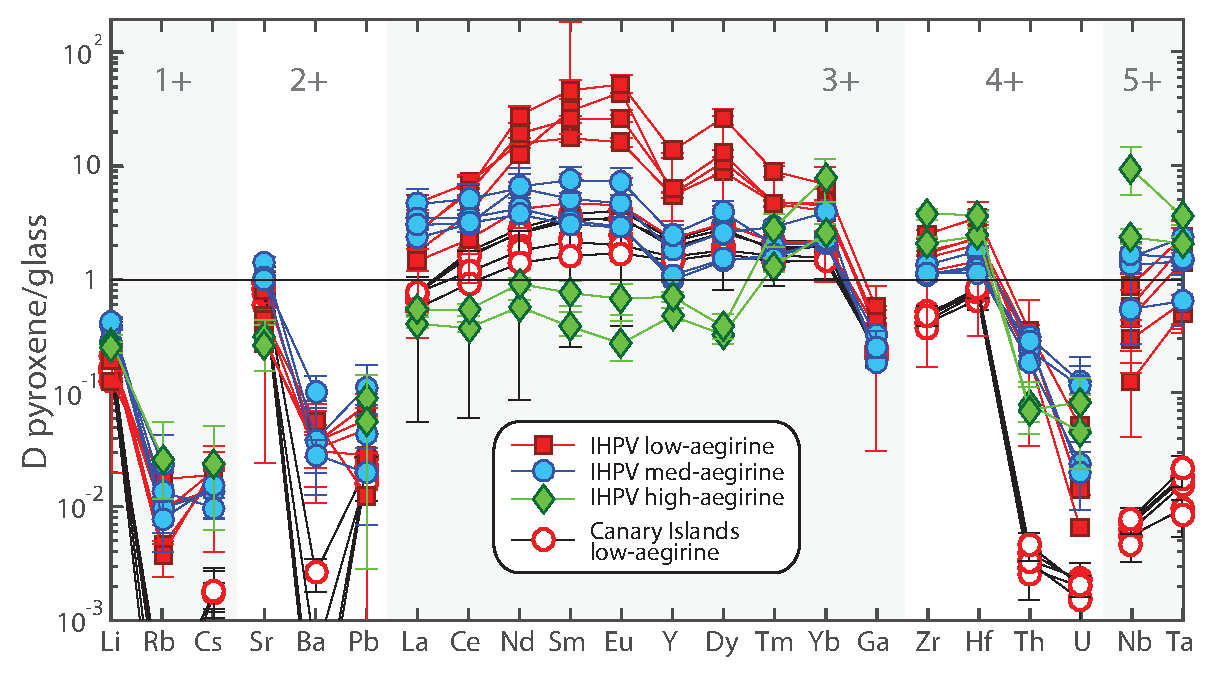
\includegraphics[width=0.75\textwidth]{6_Px_D_Spider_Apr2018.eps}
        \caption[Extended trace-element-partitioning diagram for clinopyroxene/melt]{Trace-element partition-coefficients between clinopyroxene and silicate melt, as determined from internally heated pressure vessel experiments (n = 11; low-, medium- and high-aegirine types) and from clinopyroxene-rim glass pairs from pyroclastic fall deposits from Tenerife, Canary Islands (n = 6; low-aegirine type). Uncertainties on the partition coefficients are at the 1$\sigma$ level.}
        \label{6_D_Spider}
        \end{center}
        \end{figure*}

\subsection{Trace-element-partitioning}
Apparent trace-element partition-coefficients and their uncertainties were calculated as mass concentration ratios between clinopyroxene and coexisting glass and are reported in Table \ref{D_table} and \ref{Ae_SupTbl}. 
			%Fedele:I am not sure of how these were calculated, I don't think this has been reported in the text so far. Did you use average cpx and coexisting glass data? Did you use all your data, or did you make a selection? Please add some explanation about this, I think it is necessary especially in the light of the compositional variations observed for both cpx and glass. I would also suggest that before partition coefficients are presented, some critical discussion on the data is presented in order to explain the reader how did the authors verify that the employed cpx/glass pairs can be considered to represent equilibrium pairs.
Where trace-element-concentrations in clinopyroxene could be determined using regular time-averages of counts from the ICP-MS system, a time-weighted average composition of clinopyroxene was used with that of the coexisting glass to calculate apparent trace-element partition-coefficients and their associated uncertainty (\ref{Ae_SupTbl}). Where the laser-ablation unmixing model was required for reduction of clinopyroxene trace-element analyses, the partition coefficients were calculated using time-weighted average compositions of glass alongside the corresponding `unmixed' clinopyroxene trace-element concentration (\ref{LaserMix}). Because a robust-regression data reduction scheme was used, this technique returns a median-average trace-element concentration for clinopyroxene. Derived trace-element partition-coefficients are consistent between these two data-reduction methodologies to better than 2$\sigma$. Uncertainty calculations are described in \ref{LaserMix}.

Three markedly different behaviours of rare earth element partitioning are observed in the experiments (Fig. \ref{6_D_Spider}). These depend on the aegirine concentration in the clinopyroxene and match the major-element exchange vector domains discussed above. Low-aegirine experiment clinopyroxene (\ce{Ae_{5-25}}) prefer the MREE; medium-aegirine clinopyroxene (\ce{Ae_{25-50}}) show a similar behaviour, save for higher LREE partition coefficients, whereas high-aegirine clinopyroxene (\ce{Ae_{55-95}}) strongly prefer HREE and show incompatible behaviour for the light and middle REE. The experiment REE partition coefficients are 0.3--53, typically 2--6, with minima for LREE and MREE in high-aegirine clinopyroxene (Fig. \ref{6_D_Spider}). Apparent REE partition coefficients determined from our experiments are positively correlated with the \ce{^{IV}Al} content of the clinopyroxene and are an order of magnitude higher than most literature values, the majority of which were determined for more mafic compositions (e.g. Fig. \ref{7_Al_iv}e).
	The Canary Islands clinopyroxene show similar rare earth element partitioning systematics to the low-aegirine experiment clinopyroxene, with absolute values for these partition coefficients of about one order of magnitude lower (Fig. \ref{6_D_Spider}).


        \begin{figure*}[htp]
        \begin{center}
        \includegraphics[width=0.62\textwidth]{7_D_Al_iv_Literature_Jun2017-01.eps}
        \caption[Selected trace-element-partition coefficients vs. \ce{^{IV}Al}]{Element partition coefficients for HFSE (Ti, Zr, Nb), REE (La, Sm, Yb) and TE (Li, Th) vs. \ce{^{IV}Al} (c.f.u.). Literature values (n = 411), including those from potassic Italian volcanoes (red), are from the compilation of \citet{Bedard2014}, with additional, more recent, data from \citet{Mollo2016}. Figure \ref{D_XM2Na} shows similar diagrams with $X^{M2}_{Na}$ in place of \ce{^{IV}Al}.}
        \label{7_Al_iv}
        \end{center}
        \end{figure*}
%\subsubsection{High field-strength elements}
The high field-strength elements (HFSE) Zr, Hf, Nb and Ta are compatible to slightly incompatible in the experimental clinopyroxene, and typically 1--2 orders of magnitude less compatible in the Canary Islands clinopyroxene (Fig. \ref{7_Al_iv}a,b,c).
$D_{HFSE}$ for the low-aegirine experiments and Canary Islands rocks plot on trends with the \ce{^{IV}Al} content of clinopyroxene, as defined by literature data from Italian volcanoes.
In our medium- and high-aegirine experiments $D_{HFSE}$ values are not correlated with the \ce{^{IV}Al} content of clinopyroxene, consistent with a distinct incorporation mechanism for these elements relative to the low-aegirine experiments.
%\subsubsection{LILE}
	Partition coefficients for the large-ion lithophile elements K, Sr, Pb are positively correlated with $X_{Na}^{M2}$ in the low- and medium-aegirine clinopyroxene, but are lower in high-aegirine clinopyroxene (Fig. \ref{6_D_Spider}, \ref{Ae_SupTbl}). The Rb, Cs and Ba partition coefficients have a high uncertainty and are maximum estimates owing to low concentrations of these elements in the clinopyroxene, close to the detection limit for analyses by LA-ICP-MS.
	%\subsection{actinides}
	Lithium is incompatible (\ce{D_{Li}} = 0.1--0.4) in both Canary Islands and experimental clinopyroxene and, like Sr and Pb, becomes more compatible with increasing aegirine content in the clinopyroxene, plateauing at $X_{Na}^{M2}$ = 0.4 and decreasing thereafter (Fig. \ref{D_XM2Na}g). 
	The actinides U and Th show contrasting partitioning behaviour; the former showing no correlation with aegirine content in the clinopyroxene, the latter becoming more incompatible with increasing aegirine content (Fig. \ref{7_Al_iv}h). The U and Th partition coefficients for our Canary Islands samples are similar to those for the Italian volcanoes \citep{Wood2001cpx, Fedele2009, Mollo2013, Mollo2016}, and are 1--2 orders of magnitude more incompatible relative to the experimental clinopyroxene.
	%Fedele: Again, big mismatch. Some explanation is needed (maybe in the discussion section?).

\subsection{The effects of melt structure on element-partitioning}

The partitioning of trace-elements between crystals and melts is controlled by their relative activity in each phase and the exchange mechanisms by which their incorporation into crystals takes place \citep[e.g., Jd-melt, Jd-DiHd and CaTS-DiHd exchanges have been shown to control REE incorporation in cpx, ][]{Putirka2008,Wood2014,Mollo2017}. 
In relatively polymerised systems (NBO/T $<$ 0.49), melt structure can impart a significant influence on partitioning behaviour \citep{Gaetani2004,Schmidt2006,Huang2006}. In our strongly depolymerised peralkaline system apparent partition coefficients are not correlated with NBO/T, except for $D_{Sr}$ that shows a weak positive correlation (Fig. \ref{10_1_MeltStructure}). NBO/T could not be calculated for our Canary Islands compositions because the water content of the melt prior to quench is not known.

\begin{figure*}[tp]
        \begin{center}
        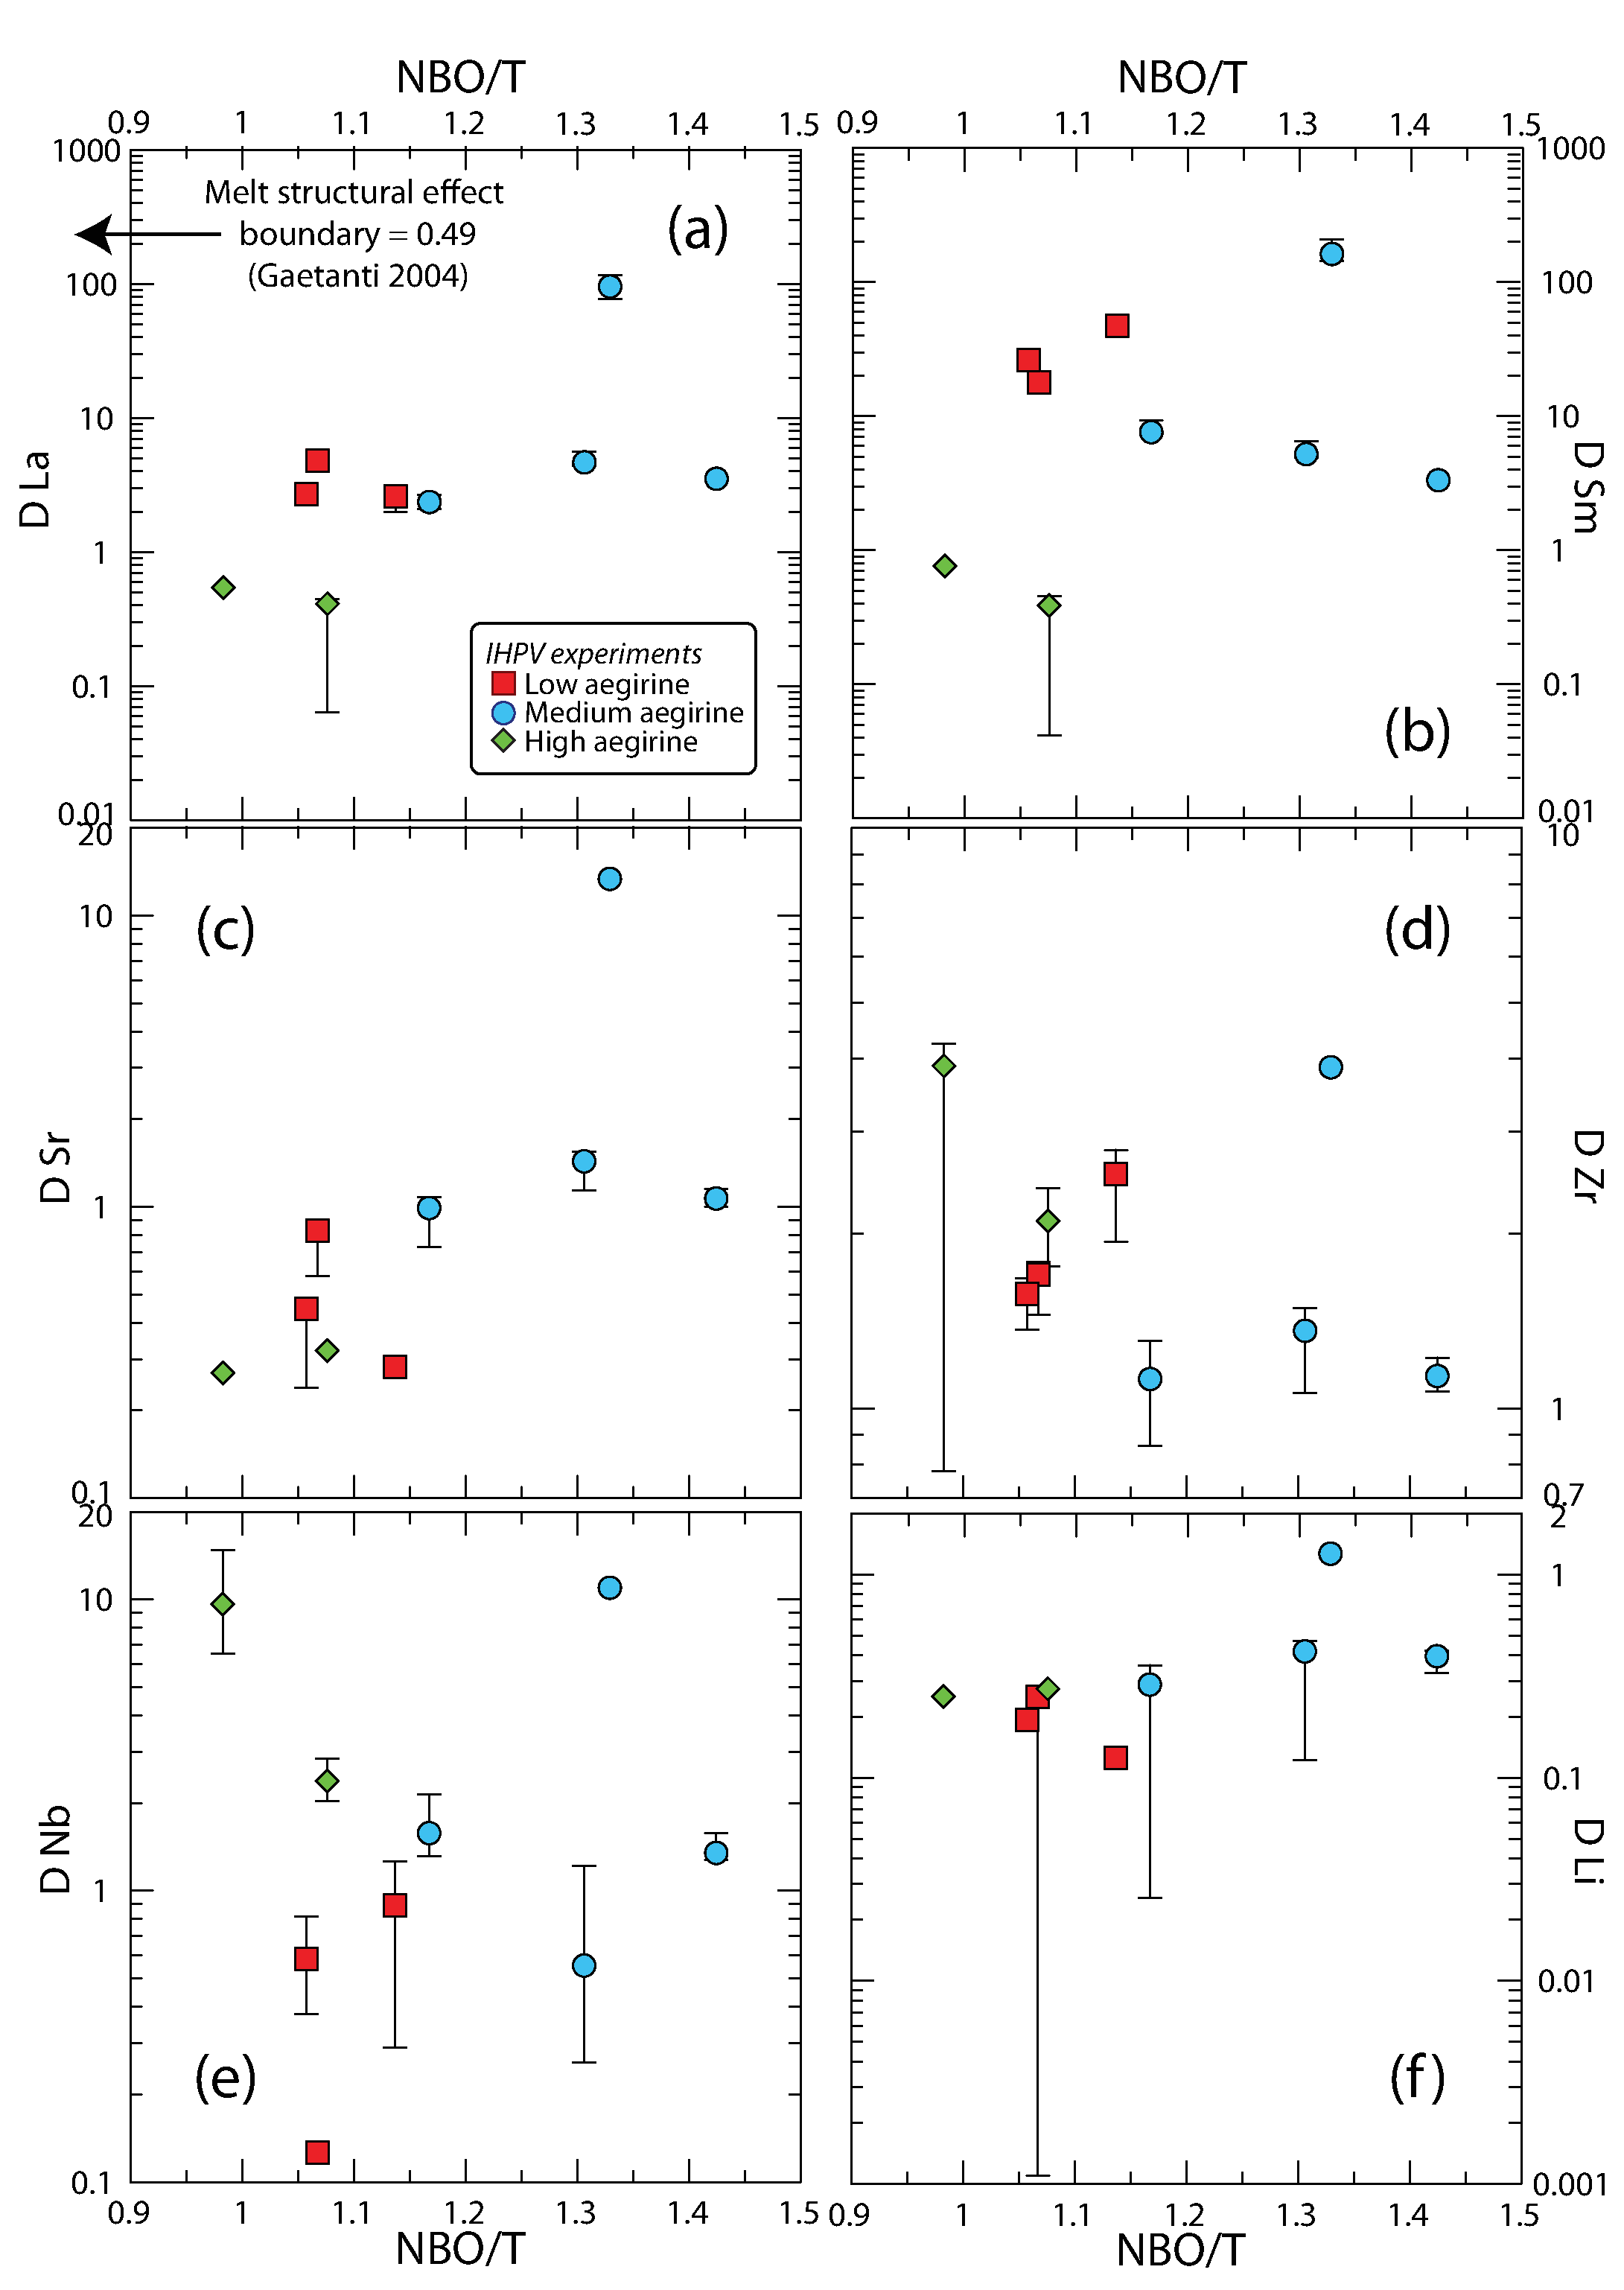
\includegraphics[width=0.8\textwidth]{11_NBO-T_Traces.eps}
        \caption[]{Diagrams of clinopyroxene--melt trace-element partition coefficients for the IHPV experiments as a function of NBO/T of the quenched melt. NBO/T was calculated following \citet{Mysen1985} with melt Fe oxidation state assigned following \citealt{Kress1991} and the water content of the melt estimated by difference from 100\% major-element oxides.}
        \label{10_1_MeltStructure}
        \end{center}
\end{figure*}


% clinopyroxene--melt element-partitioning is a process controlled by the structures of both phases, an empirical model based on both melt and mineral composition has the potential for the higher accuracy than one based on mineral composition alone. 


% However, models that require measurement of both melt and crystal compositions as input may be applied to a narrower range of geological scenarios relative to those that require crystal composition only.


% Because the structure of both melts and minerals influences trace-element-partitioning behaviour, empirical models that predicts partition coefficients based on the composition of both phases have the potential for higher accuracy than those based on mineral composition alone. 

% Despite a lower potential for accuracy, an empirical partitioning model based only on crystal composition may have greater utility than one that requires measurement of both melt and crystal compositions. This is ultimately because it may be applied where melt composition cannot be measured directly, for example in the case of concentrically zoned crystals or cumulates. 



% Fundamentally, element-partitioning is an equilibrium process that must be controlled by the composition, thus structure, of both the mineral and the melt. In the case of \citet{Huang2006}, clinopyroxene composition is relatively constant, permitting comparison of a wide range of experimental data and discussion of melt structural effects. The element-partitioning data set for strongly alkaline compositions is significantly smaller, and the range of mineral compositions much wider. We hypothesise that melt effects would influence element-partitioning in strongly alkaline systems, much like it appears to in systems of lower alkalinity. We suggest that we may not yet have the compositional resolution to isolate melt effects from mineral compositional effects in strongly alkaline systems.




 % Mollo:
 %By analogy with thermobarometers, the most common exchange equilibria are: 1) Jd-melt where the formation of Jd is accompanied by a great change in molar volume, resulting in a P-dependent reaction, and 2) Jd-DiHd and CaTs-DiHd where the volume changes for the solution of Jd and CaTs into DiHd are significantly low, leading to T-dependent reactions (see Putirka et al., 1996 for further details). It has been observed by Putirka (2008) that the thermometers based only on cpx composition have a predictive power lower than those based on cpx and melt compositions. Please notice that the Jd-melt, Jd-DiHd and CaTS-DiHd exchanges control REE incorporation in cpx, according to the literature studies. Thus, you should not write that "Models including melt parameters require additional measurements and have limited utility, relative to partitioning models requiring measurements of only one phase". In fact, you have not demonstrated this statement in your study.




\subsection{Fits to the lattice-strain model}

        \begin{figure*}[tb]
        \begin{center}
        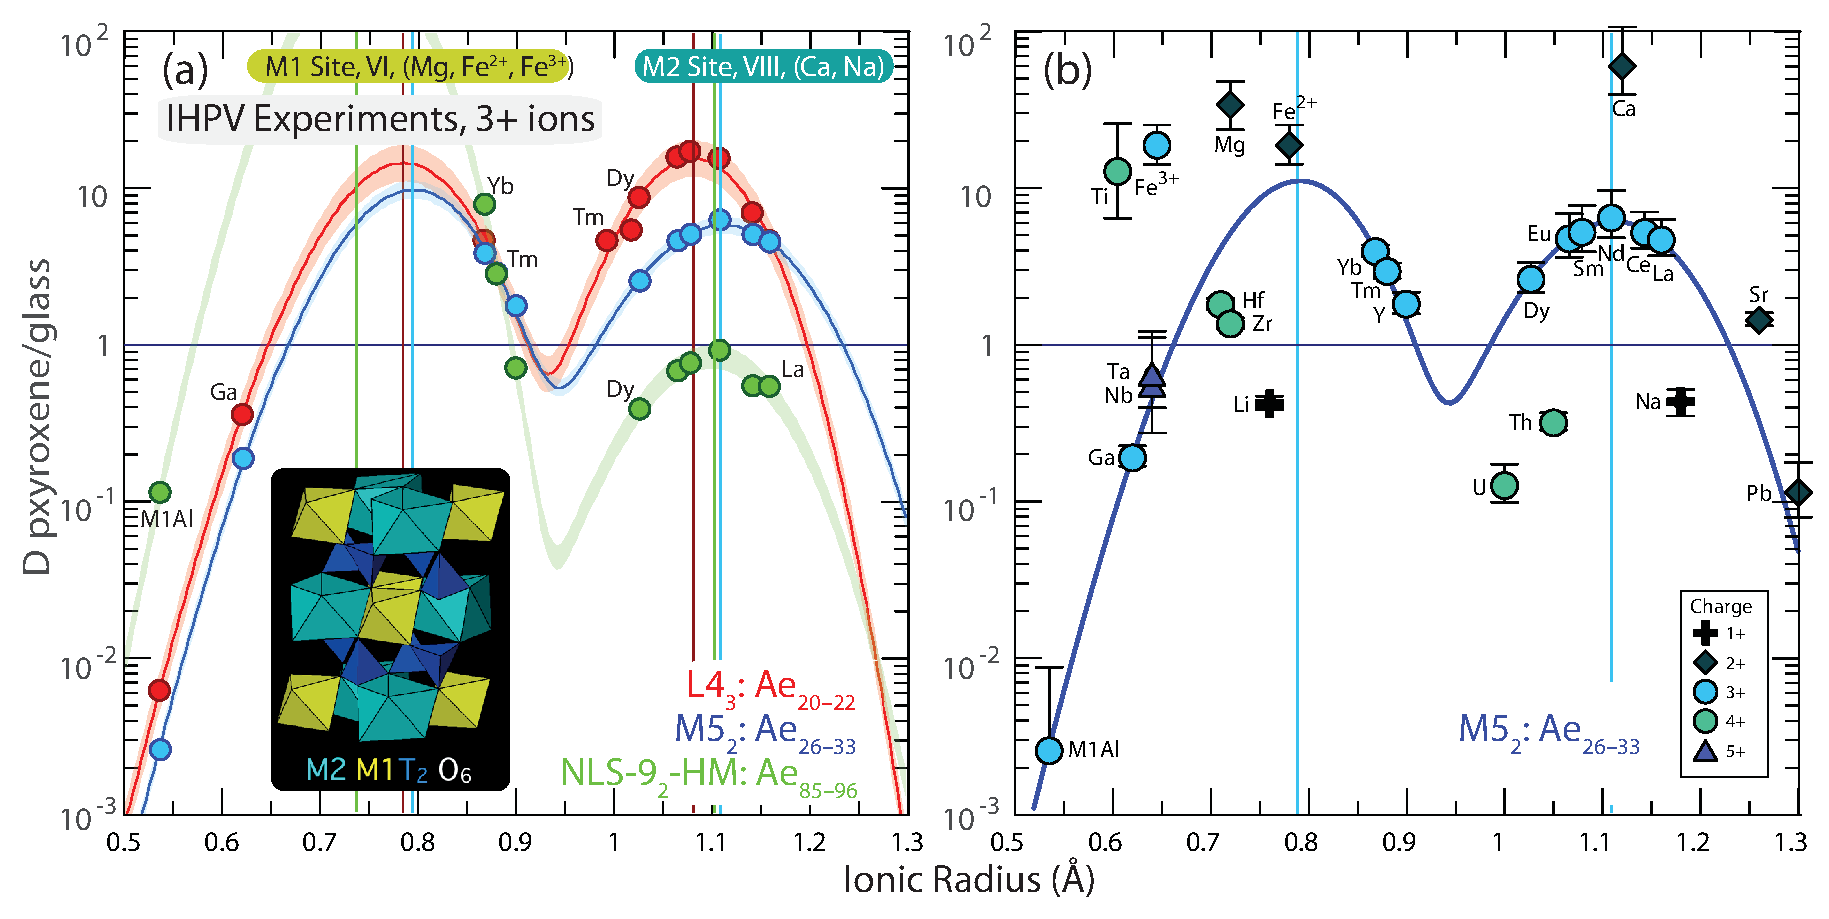
\includegraphics[width=1\textwidth]{8_Latticestrain-01.eps}
        \caption[Lattice-strain fits to \ce{R^{3+}} element-partition coefficients]{Non-linear weighted least-squares fits to element-partitioning data from the internally heated pressure vessel experiments following the lattice-strain model of \citet{Blundy1994}. (a) Representative fits to 3+ ion partitioning behaviour with examples for low (red), medium (blue) and high-aegirine (green) clinopyroxene experiments. (b) Measured partition coefficients for ions of 1+, 2+, 4+ and 5+ charges that are consistent with the lattice-strain model. Ionic radii are assigned to 6 or 8 fold co-ordination \citep{Shannon1976}, and were chosen to minimise residuals in the fit \citep[cf.][]{Olin2010}. Y was not included in the fitting routine for 3+ ions because of mass fractionation effects (ibid.).
        Vertical coloured lines indicate ideal ionic radii ($r_0$) of \ce{^{VI}M}1 and \ce{^{VIII}M}2 sites and shaded areas indicate 95\% confidence intervals on the fits determined via bootstrapping. Uncertainties on the partition coefficients in (b) are 1$\sigma$. Fitted lattice-strain parameters are given in Table \ref{D_table}.}
        \label{8_Latticestrain3}
        \end{center}
        \end{figure*}

The equilibrium partitioning of trace-elements between minerals and melts is largely controlled by the structure of the crystal lattice, its elasticity \citep{Onuma1968, Kumazawa1969, Weidner1982} and its ability to accommodate an excess or shortage in charge \citep{Blundy1998, Wood2001charge, Hanchar2001, Corgne2005CMP}. The lattice-strain model provides a framework in which the influence of these variables on partitioning behaviour can be quantified, and thus predicted under conditions bracketed by a calibrating data set \citep{Onuma1968, Blundy1994, Wood2014}. The lattice structure of minerals has a dependence on pressure, temperature and composition, and element-partitioning is a thermodynamically-controlled process \citep[e.g.][]{Wood1997}.

Most trivalent ions, including the REE and Y enter the M2 site of clinopyroxene, which is typically 6- or 8-coordinated \citep{Deer1992}. Smaller trivalent ions, including Al, Cr, Ga, Sc, and in the case of Fe-rich clinopyroxene the HREE may enter the smaller \ce{^{VI}M}1 site \citep{Olin2010, Reguir2012, Bedard2014}. The high field-strength elements Ti, Zr, Hf, Nb and Ta are typically hosted by the \ce{^{VI}M}1 site \citep{Hill2000, Hill2011, Dygert2014}.

To investigate systematics in $D_i$ values and the mechanisms by which trace-elements are incorporated into clinopyroxene, element-partitioning behaviour was explored in light of the lattice-strain theory, quantitatively described by the lattice-strain equation: 

	\begin{align} % requires amsmath; align* for no eq. number
	   D_i^{mineral/melt} = D_0 \; exp \left[\frac{-4\pi E_sN_a}{RT} \left(\frac{r_0}{2}(r_0-r_i)^2-\frac{1}{3}(r_0-r_i)^3\right)\right]\
	   \label{LST_eqn}
	\end{align}

	
\noindent where $r_0$ is the ideal radius for the lattice site, $E_s$ is the Young's modulus (i.e., the lattice site stiffness in GPa), $D_0$ is the strain-free partition coefficient, $N_a$ is Avagadro's number, $R$ is the gas constant, $T$ is temperature in Kelvin, and $r_i$ is the ionic radius of the element in question, all radii in \si{\angstrom}. We focused on 3+ ions that cover a wide range of radii and fitted lattice-strain parameters for both the \ce{^{VI}M}1 and \ce{^{VIII}M}2 sites of clinopyroxene (Fig. \ref{8_Latticestrain3}):
		
	\begin{align} % requires amsmath; align* for no eq. number
	\begin{split}
	   D_i^{cpx/melt} = D_0^{M2} \; exp \left[\frac{-4\pi E_s^{M2} N_a}{RT} \left(\frac{r_0^{M2}}{2}(r_0^{M2}-r_i)^2-\frac{1}{3}(r_0^{M2}-r_i)^3\right)\right] \\
  + \; D_0^{M1} \; exp \left[\frac{-4\pi E_s^{M1} N_a}{RT} \left(\frac{r_0^{M1}}{2}(r_0^{M1}-r_i)^2-\frac{1}{3}(r_0^{M1}-r_i)^3\right)\right]\
	\end{split}
	\label{LST_eqn_cpx}
	\end{align}
	
	\noindent Parabolae for 3+ ions were fitted for the \ce{^{VI}M}1 and \ce{^{VIII}M}2 sites using the REE, Ga and Al assigned to the \ce{^{VI}M}1 site of clinopyroxene (Fig. \ref{8_Latticestrain3}a). Fits are weighted based on uncertainties for the element-partition coefficients. HREE have higher element-partition coefficients than can predicted by substitution into the \ce{^{VIII}M}2 site, hence were fitted with ionic radii for sixfold coordination into the \ce{^{VI}M}1 site \citep[\textit{cf.}][]{Olin2010, Reguir2012,Bedard2014}.
	Lattice-strain parameters as obtained from fits to the data are shown in \ref{Ae_SupTbl}.
	
In some low-aegirine experiments and the Canary Islands rocks, lattice-strain fitting for 3+ ions at the \ce{^{VI}M}1 site was not possible, because too few HREE partitioned onto the \ce{^{VI}M}1 site of these clinopyroxene. Here, we chose to fit only lattice-strain parameters for the \ce{^{VIII}M}2 site, or fix $D_0^{3+}$ values for the \ce{^{VI}M}1 site to match those for the \ce{^{VIII}M}2 site, and fit only the $r_0$ and $E_{s}$ parameters for the \ce{^{VI}M}1 site (\ref{Ae_SupTbl)}. Fitting of element-partitioning data for 1+, 2+ and 4+ ions was less successful owing to sparse coverage of suitable radii and detection-limit issues for some elements. Partition coefficients for 1+, 2+, and 4+ elements follow radius- and charge-dependent trends consistent with lattice-strain theory and reported effects of charge on lattice-strain parameters \citep[Fig. \ref{8_Latticestrain3}b, e.g.,][]{Hazen1979, Law2000, Adam2006}.

%----------

\subsubsection{Effects of composition on ideal site size, \ce{r0}}

        \begin{figure}[bt]
        \begin{center}
        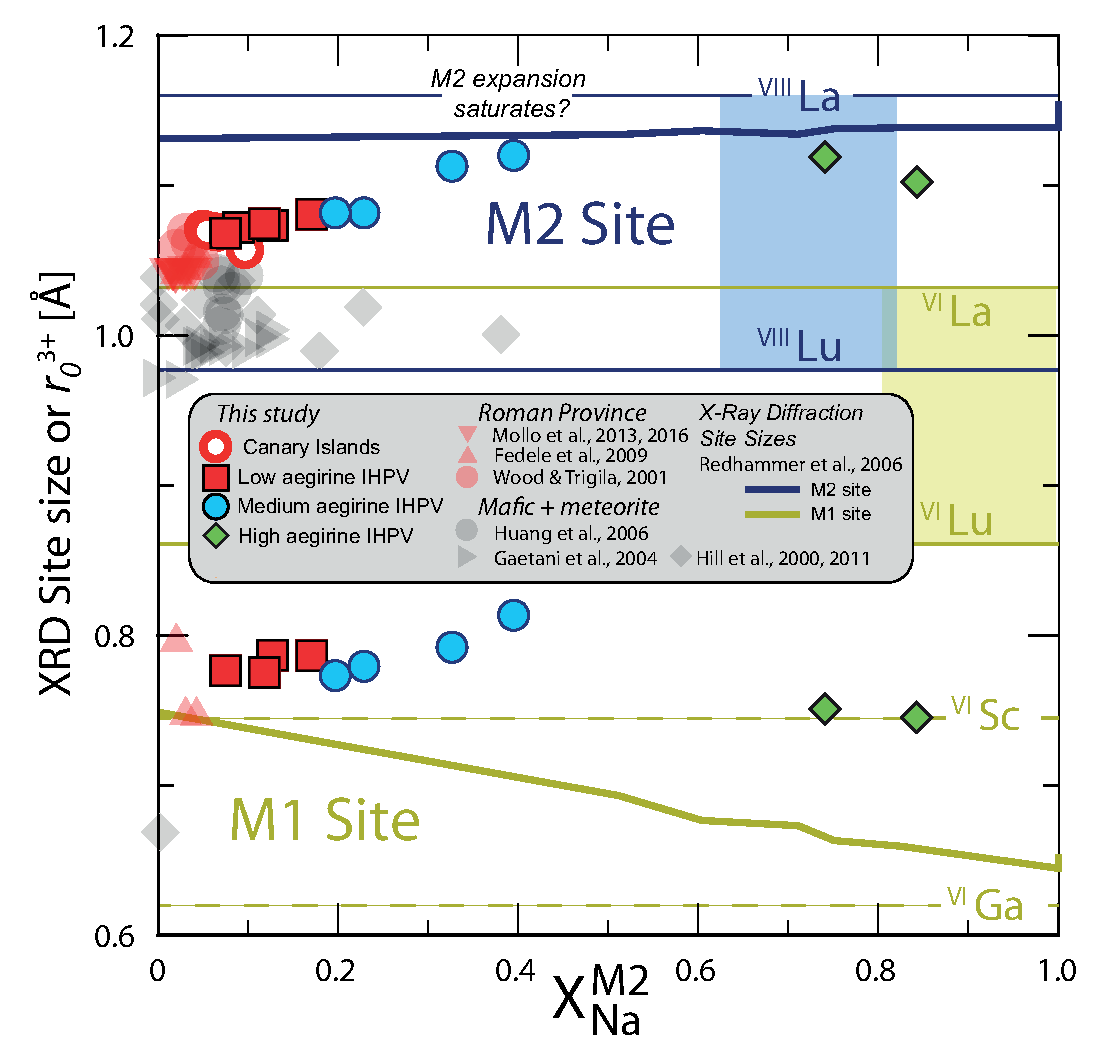
\includegraphics[width=0.45\textwidth]{9_Px_XRD_Jun2017-01.eps}
        \caption[Variation of ideal ionic radius $r_0^{3+}$ with \ce{X_{Na}}\ce{^{VIII}M}2 for \ce{^{VI}M}1 and \ce{^{VIII}M}2 sites of clinopyroxene]{Diagram showing variation of ideal ionic radius \ce{r0^{3+}} with \ce{X_{Na}}\ce{^{VIII}M}2 for \ce{^{VI}M}1 and \ce{^{VIII}M}2 sites of clinopyroxene. Shown for comparison are single crystal x-ray diffraction data from the hedenbergite-aegirine compositional join \citep[heavy solid lines, from][]{Redhammer2006}. Shaded boxes represent the range of ionic radii for rare earth elements in VI and VIII coordination \citep{Shannon1976}. Literature data for Italian volcanoes are from \citet{Fedele2009, Mollo2013, Mollo2016, Wood2001cpx} and for mafic systems are from \citet{Hill2000, Hill2011, Gaetani2004, Huang2006}.}
        \label{9_Px_XRD}
        \end{center}
        \end{figure}
        
	As the composition of clinopyroxene shifts from augite toward aegirine, the size of the \ce{^{VI}M}1 and \ce{^{VIII}M}2 sites, or strain-free radii ($r_0$), should diverge following the sizes of the major-element cations on these sites.
	Lattice-strain fits for 3+ cations indicate expansion of the \ce{^{VIII}M}2 site between low and medium-aegirine clinopyroxene, with $r_{0\, M2}^{3+}$ correlating well with Na replacing Ca (Figs. \ref{8_Latticestrain3}, \ref{9_Px_XRD}). Expansion of the \ce{^{VIII}M}2 site stalls at $r_{0\, M2}^{3+}, \approx$ 1.12 \si{\angstrom}{} and $X_{Na}^{M2} \approx 0.4$, changing little in size between medium and high-aegirine clinopyroxene. We suggest that this is a `saturation effect', whereby the smaller ions in the \ce{^{IV}T} and \ce{^{VI}M}1 sites prevent further expansion of the \ce{^{VIII}M}2 site as additional \ce{R^+_{M2}} is added to the clinopyroxene. 	
	For the \ce{^{VI}M}1 site of clinopyroxene, strain free radii for \ce{R^{3+}} cations indicate expansion between low and medium-aegirine clinopyroxene and contraction between medium and high-aegirine clinopyroxene (Figs. \ref{8_Latticestrain3}, \ref{9_Px_XRD}). These trends broadly follow the substitution of \ce{Mg^{2+}} for \ce{Fe^{2+}}, then \ce{Fe^{2+}} for \ce{Fe^{3+}} with increasing aegirine content in the clinopyroxene.
	

%--------------

\subsubsection{The effect of cation charge on the $D_0$ parameter}
 \begin{figure*}[tb]
        \begin{center}
        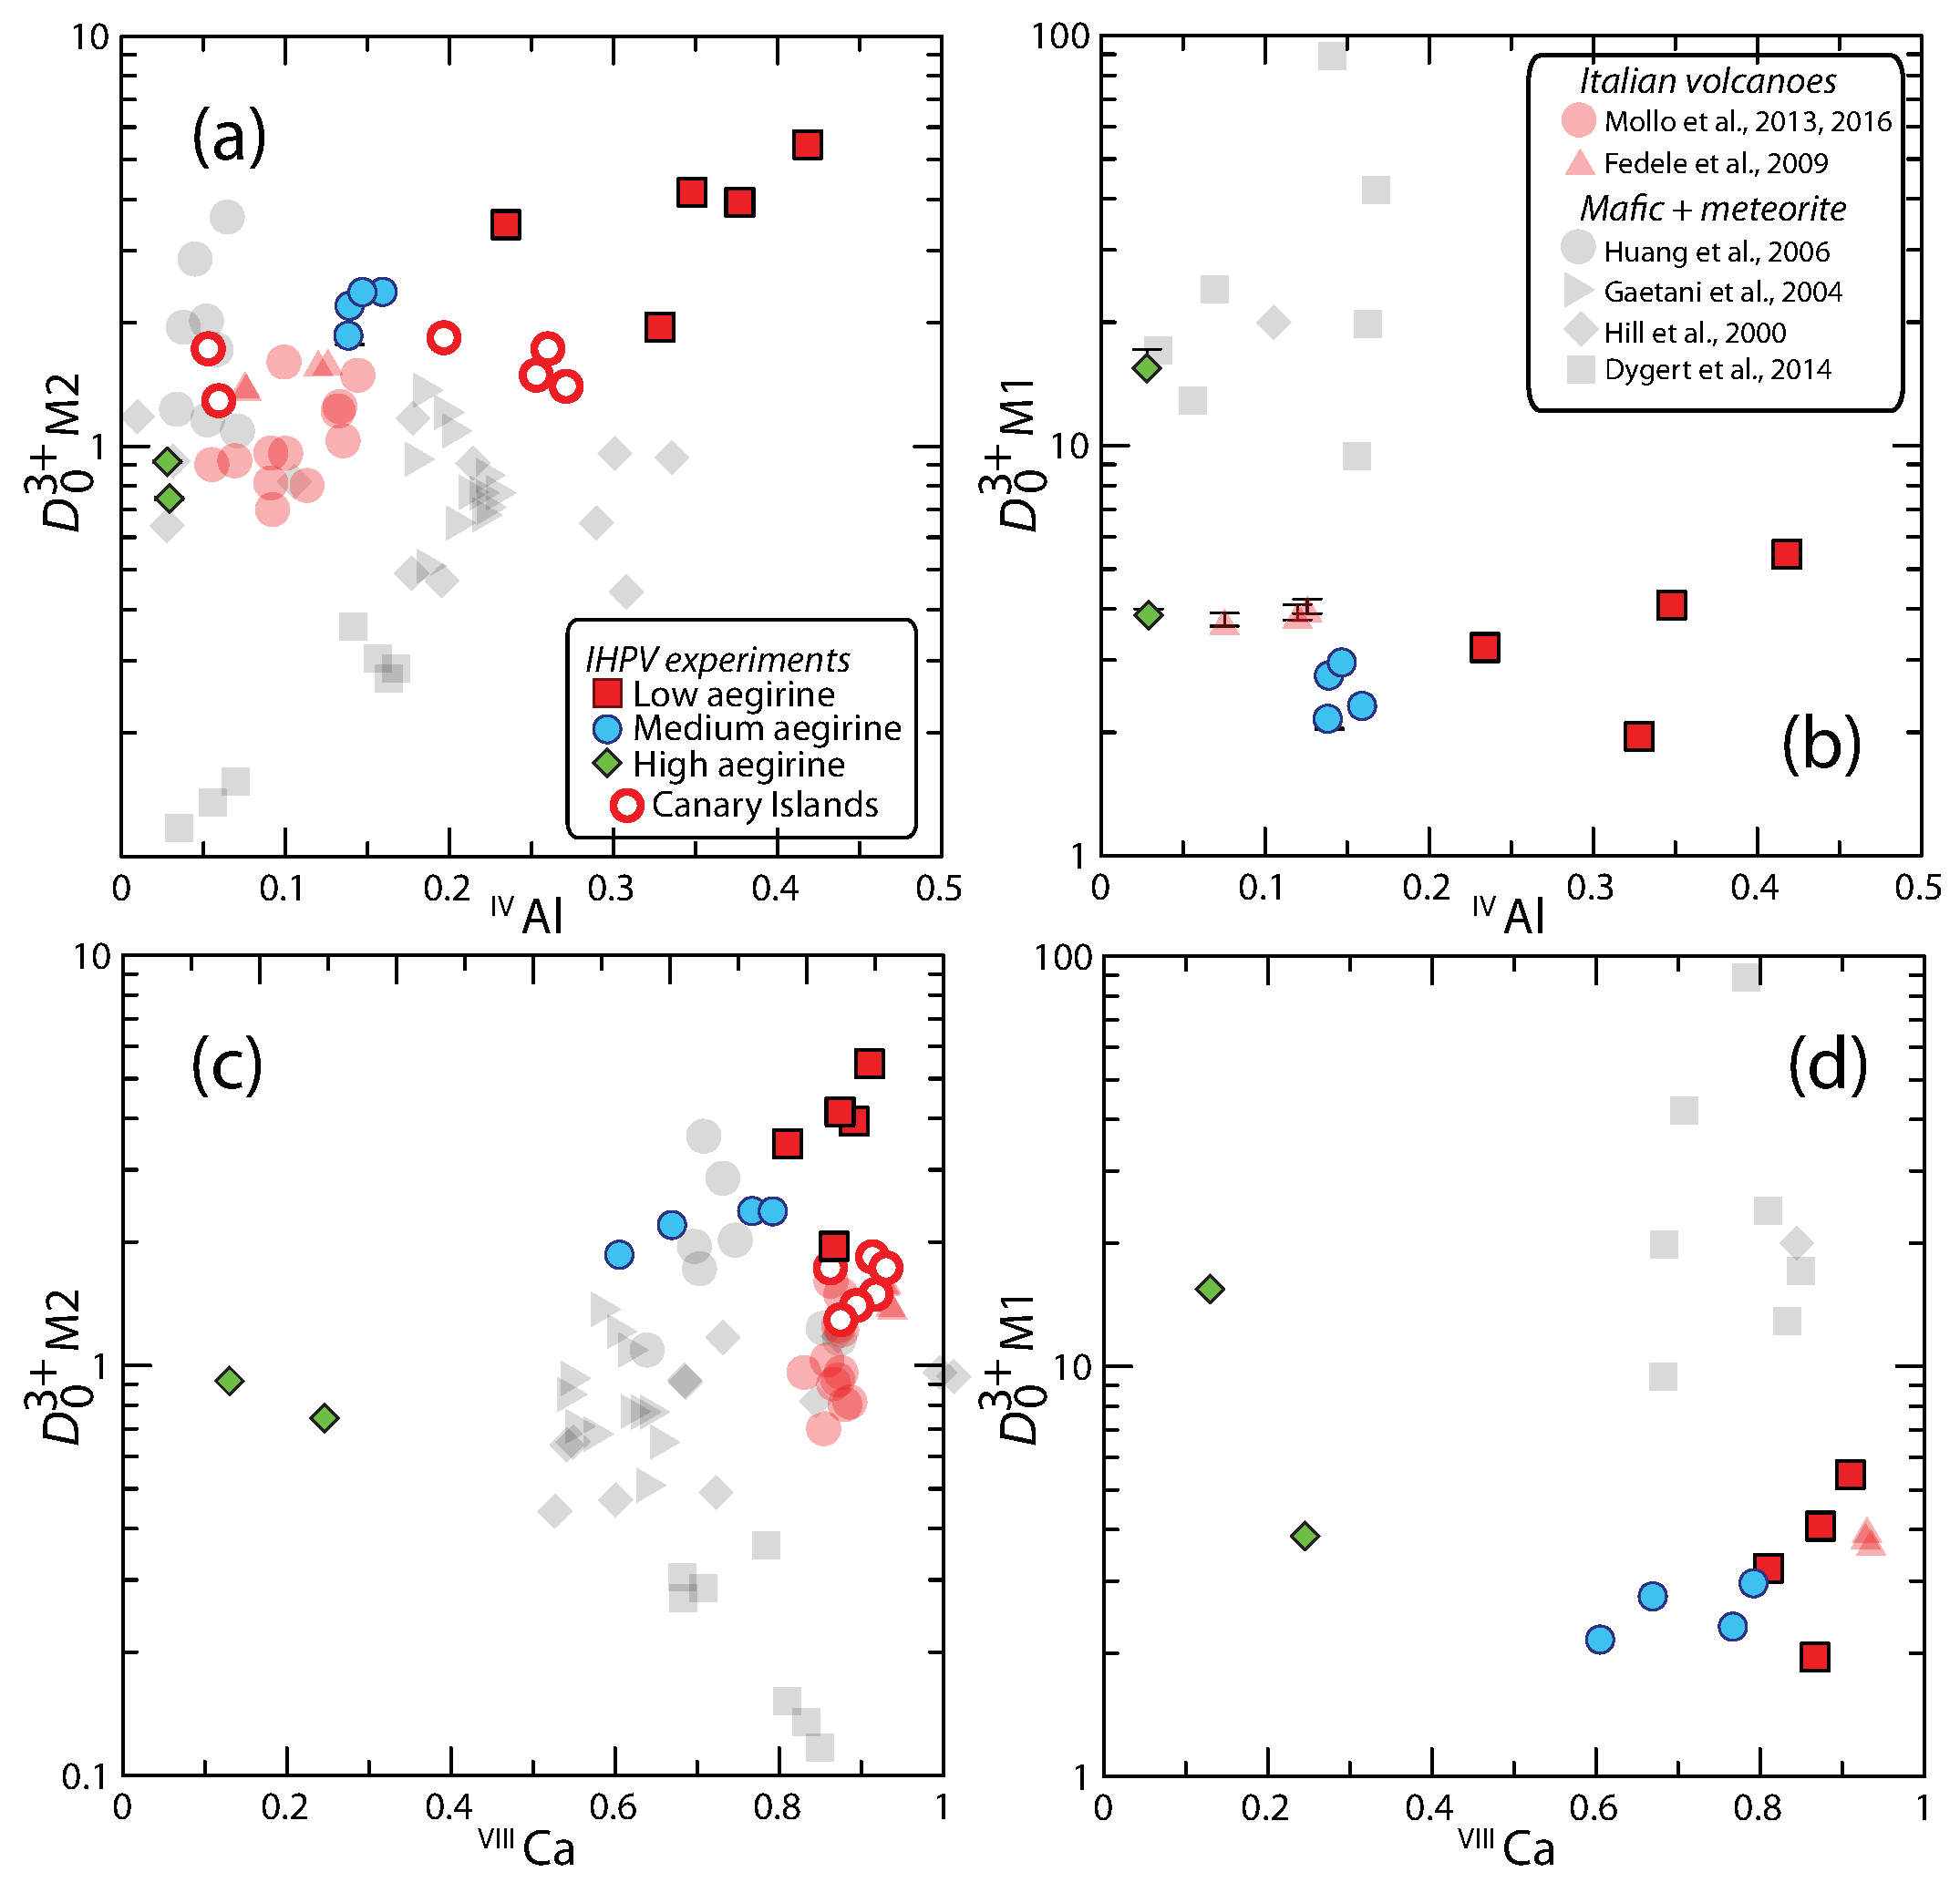
\includegraphics[width=0.8\textwidth]{10_LST_mech_Dec18.eps}
        
        \caption[Strain-free partition coefficients ($D_0$) for 3+ ions into clinopyroxene vs. various charge compensation mechanisms.]{Strain-free partitioning coefficients ($D_0$) for 3+ ions into clinopyroxene vs. clinopyroxene major-element composition. (a,c) are for the \ce{^{VIII}M}2 site, and (b,d) are for the \ce{^{VI}M}1 site. The diagrams show that variability in partitioning behaviour is highly dependent on mineral composition, and that variation between aegirine-rich clinopyroxene cannot be explained well by the same mechanisms as more mafic systems (c). Literature data for element-partitioning in Mafic + Meteorite and Italian volcano compositions are from the compilation of \citet{Bedard2014}. 1$\sigma$ uncertainties are shown in (a, b) and are usually smaller than the symbol sizes.}
        \label{10_D0_Mech}
        \end{center}
        \end{figure*}

	The $D_0$ parameter of the lattice-strain model describes ideal, strain-free partitioning and tracks the solubility of an ideal cation in the mineral with changing pressure, temperature and the bulk composition of the system \citep{Wood2014}. $D_0$ therefore correlates with the major-element composition of the clinopyroxene. Moreover, incorporation of trace-elements of a different charge introduces an electrostatic penalty that leads to a lower $D_0$ for that charge \citep{Wood2001charge, Wood2003}.
    	
	The average charge of major-elements on the \ce{^{VIII}M}2 site of clinopyroxene decreases from 2+ to 1+ on the compositional join between Ca-rich diopside and Na-rich aegirine. Consequently, the electrostatic penalty for substituting a \ce{REE^{3+}} cation into the clinopyroxene \ce{^{VIII}M}2 site is increased (Fig. \ref{10_D0_Mech}e).
	Conversely, as the average charge on the \ce{^{VI}M}1 site of clinopyroxene increases from 2+ toward 3+ in end-member aegirine, the electrostatic penalty incurred when substituting \ce{REE^{3+}} cations onto the \ce{^{VI}M}1 site is reduced (Fig. \ref{10_D0_Mech}f). $D_{0, M1}^{3+}$ consequently increases by an order of magnitude between our medium-aegirine and high-aegirine experimental clinopyroxene, an effect that when combined with the shrinking \ce{^{VI}M}1 site size, leads to strong fractionation of the HREE (Figs. \ref{8_Latticestrain3} and \ref{10_D0_Mech}f).

	A positive correlation between \ce{^{IV}Al} and partition coefficients for highly charged trace-elements has been extensively documented in studies on clinopyroxene \citep{Lundstrom1994, Gaetani1995, Blundy1998, Francis2008, Hill2011, Mollo2016}. The low-aegirine experimental clinopyroxene and most of the Canary Islands rocks extend trends defined by clinopyroxene from mafic systems (Figs. \ref{7_Al_iv}, \ref{10_D0_Mech}a), whereas the remainder of the experimental data set and Canary Islands rocks show element-partitioning behaviour similar to Italian volcanoes \citep{Wood2001cpx, Fedele2009, Mollo2016}, confirming that an \ce{^{IV}Al}-controlled substitution mechanism for REE extends to peralkaline conditions (Figs. \ref{7_Al_iv}, \ref{10_D0_Mech}a).
		

		%Kill the below parag? (CB, 13 Dec 2018)
	%\ce{^{IV}Al} is thought to facilitate incorporation of \ce{REE^{3+}} cations onto the \ce{^{VIII}M}2 site of clinopyroxene by replacing \ce{Si^{4+}}, thereby reducing local charge and thus the electrostatic penalty associated with incorporation of REE \citep{Blundy1998}. The substitution of \ce{Fe^{3+}} for \ce{^{IV}Si^{4+}} can be expected to have a similar effect. Conversely, \ce{R^{3+}} ions on the neighbouring \ce{^{VI}M}1 site should hinder incorporation of REE on the \ce{^{VIII}M}2 site, because they increase local charge by replacing \ce{R^{2+}} ions, such as \ce{Mg^{2+}} and \ce{Fe^{2+}}. This electrostatic penalty should apply doubly to \ce{Ti^{4+}} on the \ce{^{VI}M}1 site. This effect is consistent with our experimental data (Fig. \ref{10_D0_Mech}c), but is not obvious in the natural samples, nor in the majority of the literature experimental data. It would thus appear that other factors, such as melt structure, have a stronger control on $D_{REE}$ \citep[e.g.][]{Prowatke2005}.
    
	$D_0^{3+}$ parameters for the \ce{^{VI}M}1 site are strongly correlated with those for the \ce{^{VIII}M}2 site, except at aegirine concentrations exceeding 50 mol.\%. Similarities to \ce{^{VIII}M}2 partitioning behaviour likely reflect the dominance of T-site substitution mechanisms in augite clinopyroxene. In the high-aegirine clinopyroxene, T-site substitutions become less important as the T-sites become saturated with \ce{Si^{4+}} (Fig. \ref{ExchMechBar}). The replacement of \ce{Fe^{3+}} at the \ce{^{VI}M}1 site by 3+ trace-elements does introduce a charge penalty, therefore $D_{0\, M1}^{3+}$ increases accordingly.
  
%%%%%%%%%%%%%%%%%%%%
%%%%%%%%%%%%%%%%%%%%




%----------------------------

\subsection{An element-partitioning model extending to aegirine clinopyroxene}

	Partition-coefficients vary systematically with the physicochemical conditions of natural and synthetic magmas \citep[cf.][]{Wood2003}. Consequently, a host of models have been presented to describe the systematics of element-partitioning between clinopyroxene and silicate melts \citep{Wood1997, Wood2001charge, Hill2011, Yao2012, Sun2012, Bedard2014, Dygert2014, Mollo2016}. The majority of these models are based on lattice-strain theory and predict how the lattice parameters $r_0, E_s$, and $D_0$ vary with composition, temperature and pressure. This semi-thermodynamic approach theoretically permits calculation of partition coefficients for any trace-element, at any set of $P-T-X$ conditions. In reality, all models have a limited working range, as restricted by the input data set. 
	Because existing partitioning models do not reproduce the high $r_{0, M2}^{3+}$ values for clinopyroxene with aegirine contents $\geq$ 50 mol \% (Fig. \ref{12_MLModel}a), they cannot accurately predict REE partitioning behaviour for strongly peralkaline systems. 
We therefore present a new empirical model that is calibrated on both our experimental work and natural partition coefficients from Canary Islands rocks (n = 16), as well as existing partitioning data from the literature (n = 75, compilation of \citealt{Bedard2014}, and \citealt{Mollo2016}, Fig. \ref{12_MLModel}, \ref{Ae_SupTbl}). 
	Our calibration database covers a wide range of composition, pressure, temperature and oxygen fugacity (0.0001--3.5 GPa, 650--1345 \dgC, log \fO = IW to MH $\approx$ $\Delta$QFM -5 to +5). Clinopyroxene compositions are $X$Mg 0.031--1, $X_{Na}^{M2}$ 0--0.84 and \ce{^{IV}Al} 0--0.49 c.f.u. and melt composition varies widely in terms of Mg\# (0--100) and $X$\ce{H2O} (0--0.38). REE partition coefficients are \ce{$D$_{La}} 0.01--4.79; \ce{$D$_{Sm}} 0.02--47.24, and \ce{$D$_{Yb}} 0.11--8.00. The majority of partition coefficients in the training data set were measured via SIMS or LA-ICP-MS, minimising analytical uncertainty (e.g. from analyses by electron-microprobe).

Our model is based on clinopyroxene composition alone so that it may be applied in geological scenarios where melt composition cannot be directly measured, for example to the cores of zoned phenocrysts in tephra, or to cumulate systems.
	Partition coefficients between clinopyroxene and melt are controlled by the relative activity of elements in each of these two phases \citep{Wood2014}, therefore an empirical model to predict partition coefficients from both melt and mineral compositional terms has the highest potential for accuracy. 
%While melt structure has been shown to influence element-partitioning \citep{Gaetani2004, Huang2006, Schmidt2006, Mollo2017}, it is not always possible to measure melt composition directly. 
	Our approach is valid because crystallisation is a thermodynamically-controlled process and the composition of the melt and thus its effects on element-partitioning are, at least in part, recorded by the major-element composition of the clinopyroxene.

	
\subsubsection{The clinopyroxene M2 site}		
	To find the principal physicochemical factors that affect element-partitioning at the \ce{^{VIII}M}2 site of clinopyroxene, a stepwise least-squares multiple linear regression analysis was performed using the lattice-strain parameters $r_0^{3+}$, $E_s^{3+}$ and $D_0^{3+}$, temperature, pressure and clinopyroxene composition as inputs. Input parameters were initially examined in binary scatter diagrams to ascertain whether correlations with lattice-strain parameters were linear. If not, interaction compositional terms were added to the initial set of possible fitting parameters that had linear correlations with lattice-strain parameters (e.g. $X^{T}_{Al + Fe^{3+}}$). Intensive variables for multiple regression models for $r_0$, $E_s$ and $D_0$ were introduced following a hierarchical forward selection criterion with switching. The largest number of significant terms to describe a lattice-strain parameter was eight for $E^{M2}$ (c.95\%, cf. \ref{Sup_RegressionReport}).
		
%----------------Modelling results -----------------
	The resultant empirical model accounts well for changes in lattice-strain parameters over a range of compositions from basalt to peralkaline phonolite, faithfully reproducing large $r_0^{M2}$ values typical for sodic clinopyroxene (Fig. \ref{12_MLModel}a, model coefficients in Table \ref{Coeff_Table}). Student t-tests show that all of the independent variables included in the models are significant at the 95\% confidence level and PRESS $R^2$ values obtained by repeated random subsampling of the dataset \citep{Stevens1996} are close to $R^2$ values calculated by regular methods, indicating that the models are robust and have high predictive power. Full multiple regression reports are available in \ref{Sup_RegressionReport}. Equations generated by the multiple linear regression calculations are given below for the \ce{^{VIII}M}2 site, where $a_i$ are the regression coefficients for the respective variables: \\
	
		\begin{align} % requires amsmath; align* for no eq. number
	\begin{split}
   lnD^{M2}_0 = a_1 + a_2T + a_3X^{T}_{Al + Fe^{3+}} + a_4X^{M1}_{Ti} + a_5X^{M1}_{Al - Fe^{3+}} + a_6X^{M2}_{Fe^{2+}}
   	\end{split}
	\label{D0M2_eqn}
	\end{align}
	
	\begin{align} % requires amsmath; align* for no eq. number
	\begin{split}
	E^{M2} = a_7 + a_8P + a_9X^{T}_{Al + Fe^{3+}} + a_{10}X^{M1}_{Al} + a_{11}X^{M1}_{Mg} + a_{12}X^{M1}_{Ti} \\ + a_{13}X^{M2}_{Mg} + a_{14}X_{Mg}
	\end{split}
	\label{EM2_eqn}
	\end{align}
	
	\begin{align} % requires amsmath; align* for no eq. number
	\begin{split}
	r^{M2}_0 = a_{15} + a_{16}T + a_{17}X^{M1}_{Al - Fe^{3+}} + a_{18}X^{M1}_{Ti} + a_{19}X^{M2}_{Ca} + a_{20}X^{M2}_{Na}
	\end{split}
	\label{r0M2_eqn}
	\end{align}
	   
	   
	      %\begin{landscape}
        \begin{sidewaysfigure*}[p]
        \begin{center}
        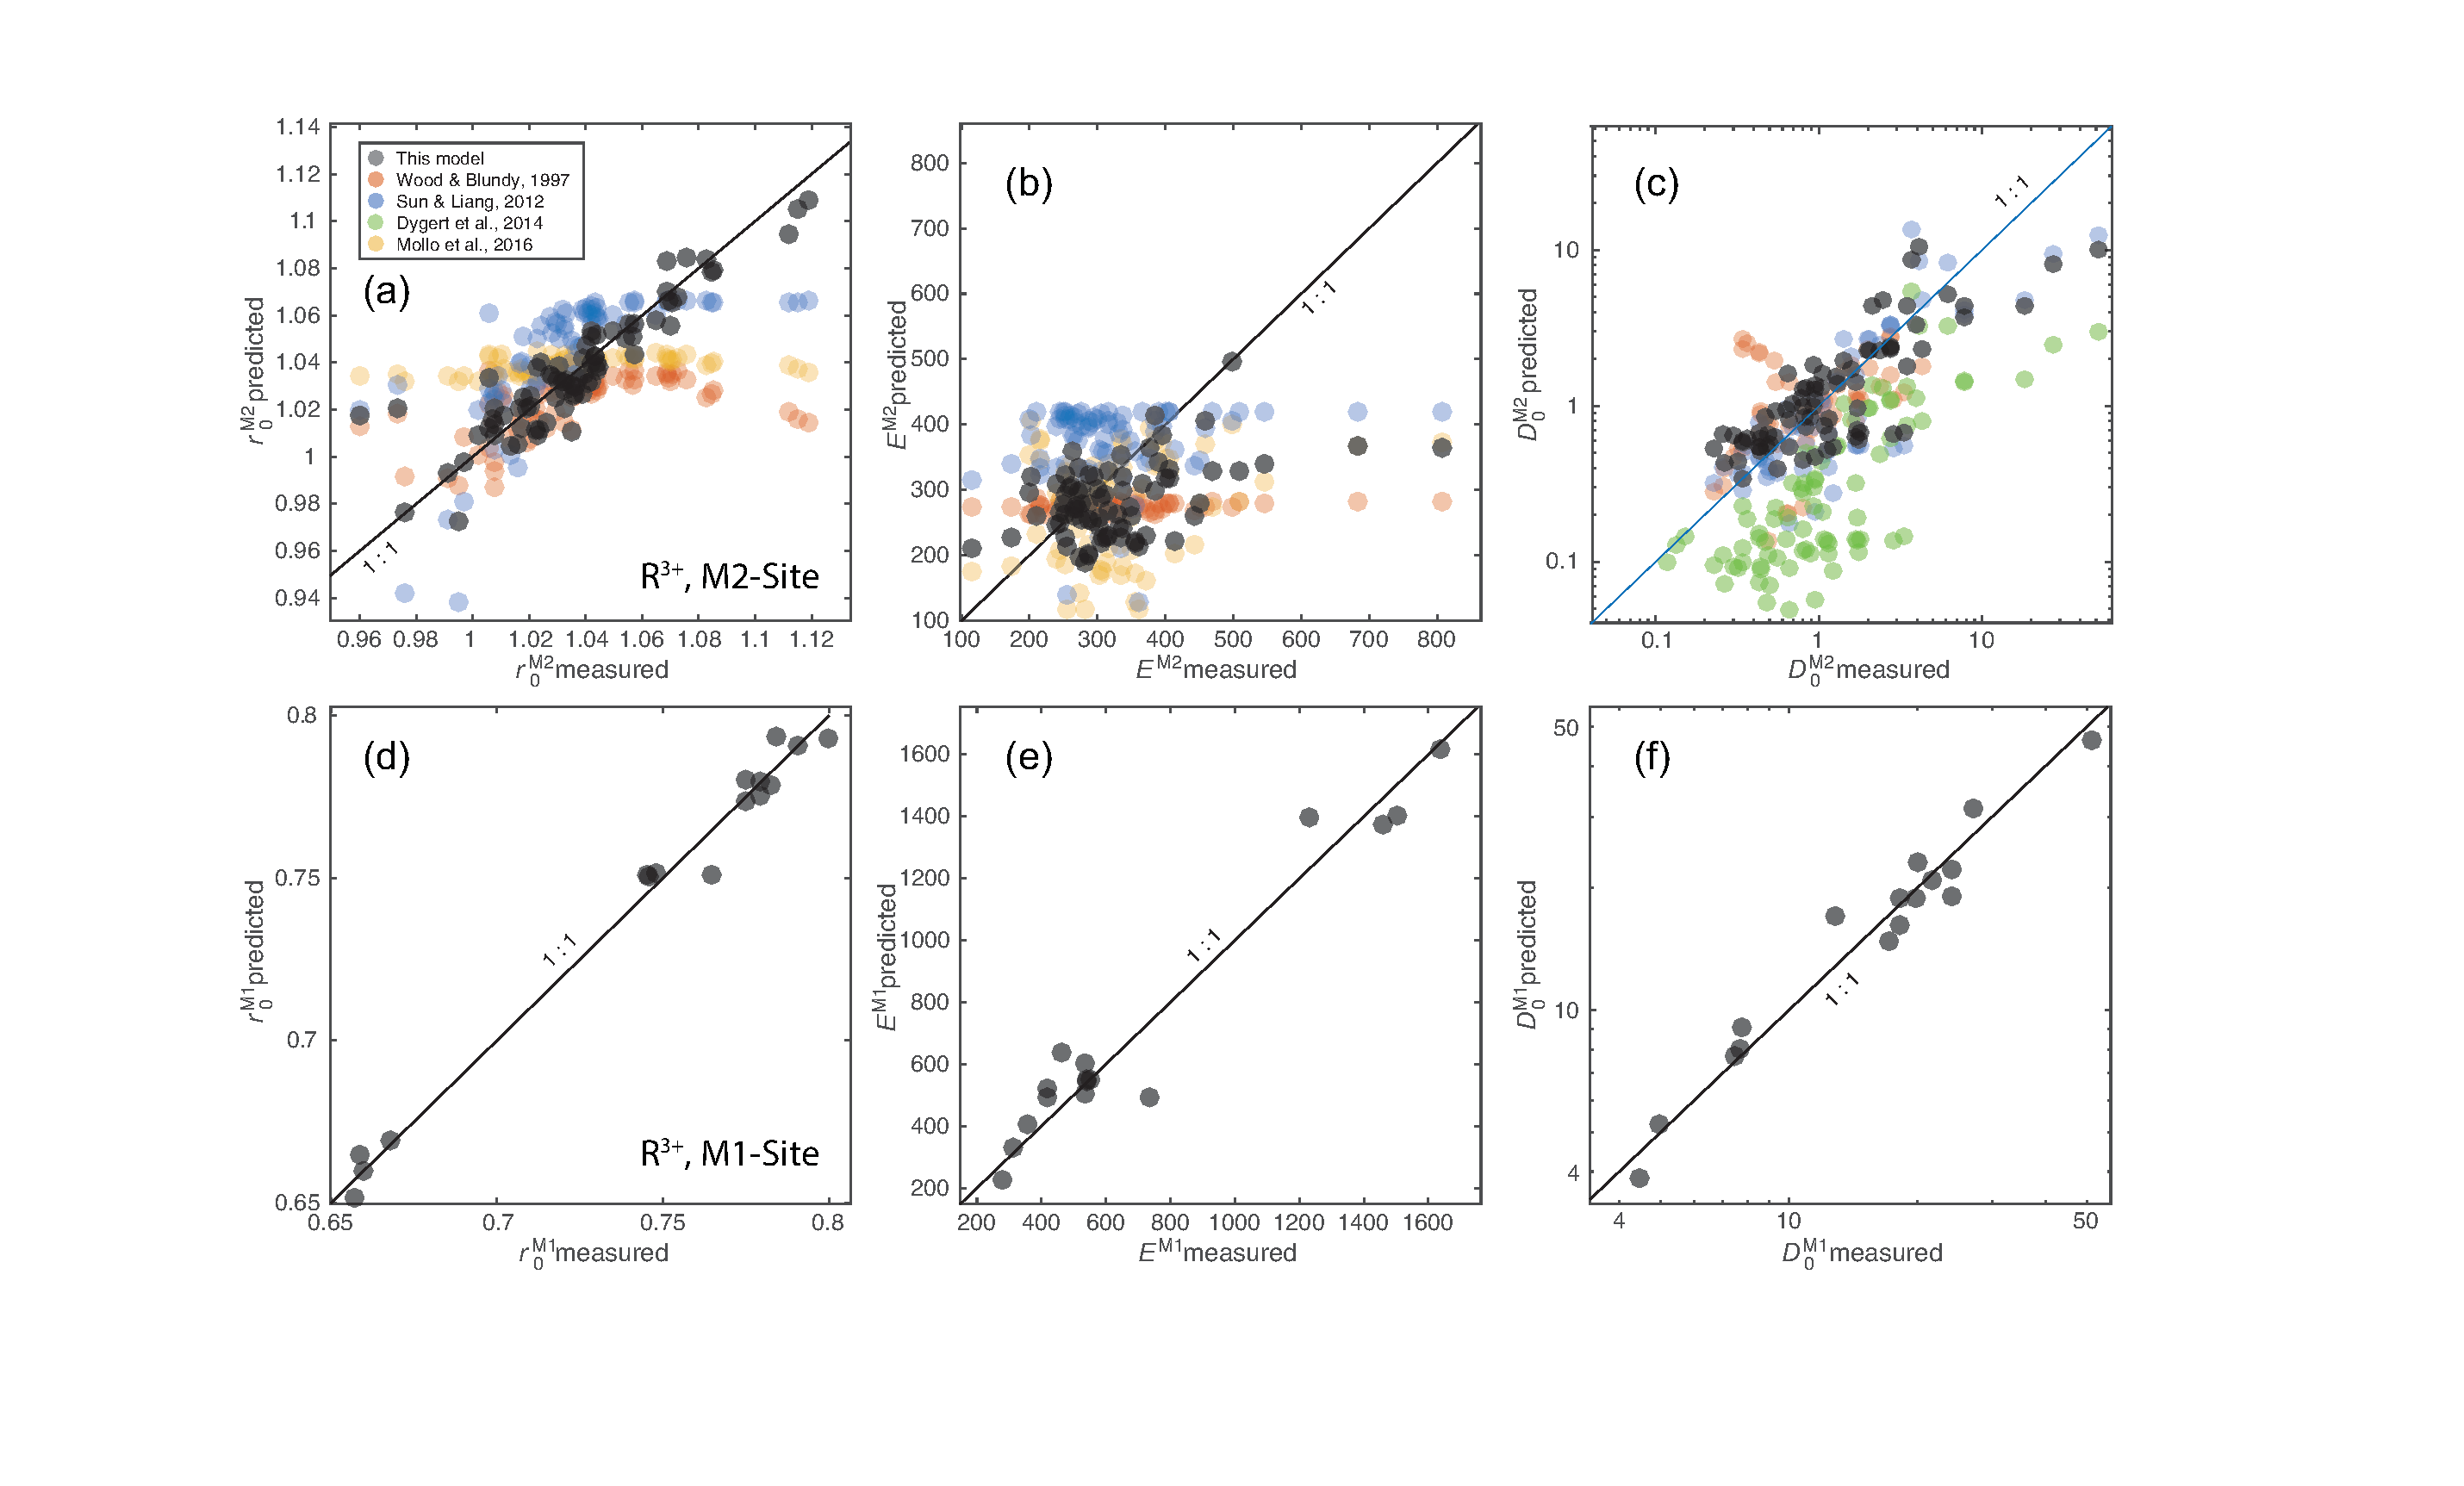
\includegraphics[width=1\textwidth]{12_StepwiseMultilinear_M1M2_24Oct2017.eps}
        \caption[Measured vs. predicted model values for lattice-strain parameters for the \ce{^{VIII}M}2 and \ce{^{VI}M}1 sites of clinopyroxene]{Measured vs. predicted model values for lattice-strain parameters for the \ce{^{VIII}M}2 and \ce{^{VI}M}1 sites of clinopyroxene. The new models presented here were generated via a stepwise multiple linear regression procedure following a hierarchical forward selection criterion with switching. Full regression reports are in \ref{Sup_RegressionReport} and model equations are in the main text.
        }
        \label{12_MLModel}
        \end{center}
        \end{sidewaysfigure*}
       % \end{landscape}

	   
%Modelling results continued----------------------

%Mollo review: You always refer to general adjectives (good, well, low, high etc.) with the aim to describe the predictive power of your model. Report the most important statistical values in the main body of the manuscript.
The model for $r_0^{M2}$ is robust with high predictive power and incorporates compositional controls from the \ce{^{VI}M}1 and \ce{^{VIII}M}2 sites, as well as temperature. Elevated concentrations of large \ce{^{VIII}M}2 cations \ce{Ca^{2+}} and \ce{Na+} are correlated with large \ce{^{VIII}M}2 sites. \ce{Ti^{4+}} cations in the neighbouring \ce{^{VI}M}1 site are also correlated with expansion of the \ce{^{VIII}M}2 site, and the concentration of small \ce{Al^{3+}} minus larger \ce{Fe^{3+}} on the \ce{^{VI}M}1 site is negatively correlated with $r_0^{M2}$. The negative correlation between $r_0^{M2}$ and temperature reflects the sum of changes to major-element composition that lead to smaller clinopyroxene \ce{^{VIII}M}2 sites at higher temperatures. This compositional effect swamps the minor influence of thermal expansion.

The model for $D_0^{M2}$ incorporates compositional terms from all three sites in clinopyroxene and temperature. The positive effect of tetrahedral \ce{R^{3+}} on $D_0^{M2}$ is the largest contribution to the model, which is consistent with published studies (see above). The relationship between clinopyroxene compositional terms on the \ce{^{VI}M}1 and \ce{^{VIII}M}2 sites and $D_0$ are indirect and are tied to the solubility of the mineral in the melt \citep{Wood2003}, which in turn is tied to the physicochemical conditions of the system (largely melt composition). The model for $D_0^{M2}$ is less robust that that for $r_0^{M2}$, largely because there are melt compositional effects that are not recorded in the composition of the clinopyroxene. We tested the Mg\# and $X$\ce{H2O} of the melt, neither of which are significant predictors for $D_0^{M2}$ (95\% confidence interval).

The model for $E^{M2}$ is less well-constrained than for the other two \ce{^{VIII}M}2 lattice-strain parameters, suggesting that \ce{^{VIII}M}2 site stiffness is not tied strongly to clinopyroxene composition, temperature or pressure. Despite a significantly lower predictive power, this model still has physical grounding. Stiffness of the \ce{^{VIII}M}2 site is positively correlated with pressure, as might be expected following a simple Hooke's law relationship, and there are some subtle compositional controls imparted by the \ce{^{IV}T} and \ce{^{VI}M}1 sites. The poor correlation between $E^{M2}$, clinopyroxene composition, temperature and pressure is also evident in published element-partitioning models, where $E^{M2}$ is either poorly predicted (Fig. \ref{12_MLModel}b), or set to a fixed value \citep[e.g.][]{Dygert2014}.

Diagrams of measured vs. predicted $D$ values for \ce{R^{3+}} cations are given in Figure \ref{13_GlobalInv}a, showing the predictive power of the models over a compositional range between basalt and peralkaline phonolite. For the \ce{^{VIII}M}2 site, 95\% of the measured \ce{R^{3+}} partition coefficients are reproduced within a factor of $\frac{+ 2.5}{- 2.9}$ (hard dashed lines), and in extreme cases, the model still reproduces $D$ values within an order of magnitude, sufficient for the prediction of element-partitioning trends over a wide range of $P-T-X$. $D_{MREE}$, such as Sm, are reproduced more faithfully than $D_{LREE}$, because their radius is closer to $r_0^{M2}$ (Fig. \ref{13_GlobalInv}c,d), and therefore prediction of their partitioning behaviour is affected less strongly by inaccuracies in predicted $E^{M2}$ values.

%%%%%%%%%%%%%%%%%%%%%%%%%
%%%%%%%%%%%%%%%%%%%%%%%%%

 \begin{figure*}[tp]
        \begin{center}
        \includegraphics[width=0.65\textwidth]{13_13thOct_VvHmodel_M1M2-02.eps}
        \caption[Measured clinopyroxene--silicate melt partition coefficients for 3+ cations vs. those predicted by our empirical model.]{Measured clinopyroxene--silicate melt partition coefficients for 3+ cations vs. those predicted by our empirical model.
        (a) shows a comparison between measured partition coefficients and model-derived values for the \ce{^{VIII}M}2 site of clinopyroxene. Hard dashed lines represent 95\% confidence intervals of the model, and correspond to maximum uncertainties of factor $\frac{+ 2.5}{- 2.9}$. Fine dashed lines represent 1 order of magnitude uncertainty (extreme outliers for \ce{^{VIII}M}2 model). Partition coefficients in this diagram are the REE La to Er for our IHPV experiments, Canary Islands rocks, and literature data from the Italian volcanoes \citep{Wood2001cpx,Fedele2009,Mollo2013,Mollo2016}, and all the REE plus Y for the rest of the data compilation \citep{Bedard2014}, which is split by analytical methodology. (b) shows performance of the predictive model for the \ce{^{VI}M}1 site that is calibrated for alkaline magmatic systems, and includes data from our IHPV experiments and the Italian volcanoes \citep{Fedele2009,Mollo2013,Mollo2016}. Maximum uncertainties at the 95\% confidence interval are a factor of $\frac{+7}{-11}$, higher than for the \ce{^{VIII}M}2 site because of the smaller calibrating data set. (c) performance of the \ce{^{VIII}M}2 site model for La, and (d) for Sm.}
        %Reviewer2: which partitioning data are examined here? Does the Dygert et al. model fail to reproduce their own data? Problem with the calculation here? 
        %Also, isn't the D0 inverted rather than measured?
        \label{13_GlobalInv}
        \end{center}
        \end{figure*}

\subsubsection{The clinopyroxene M1 site}
Using a methodology similar to the \ce{^{VIII}M}2 site, we fitted a predictive model for partitioning of \ce{R^{3+}} cations onto the smaller \ce{^{VI}M}1 site of clinopyroxene. Lattice-strain parabola were constrained by partitioning data for Cr, Ga, Sc, and where suitable, the HREE Tm, Yb and Lu (Our IHPV experiments plus \citealt{Hill2000, Fedele2009, Mollo2013, Dygert2014}). The training data set for the \ce{^{VI}M}1 site partitioning model is small relative to that for the \ce{^{VIII}M}2 site (n = 18), and because it is strongly skewed toward alkaline compositions, it has lower predictive power and is not recommended for application to mafic magmatic systems. Equations for the \ce{^{VI}M}1 site lattice-strain parameters, as generated by multiple linear least squares regression, are given below and shown in Figure \ref{12_MLModel} where $b_i$ are the regression coefficients (Table \ref{Coeff_Table}) for the respective variables:
 
     \begin{align} % requires amsmath; align* for no eq. number
	\begin{split}
   lnD^{M1}_0 = b_1 + b_{2}X^{T}_{Al} + b_3X^{M1}_{Fe^{3+}} + b_4X^{M2}_{Ca} + b_5X^{M2}_{Na}
   	\end{split}
	\label{D0M1_eqn}
	\end{align}
	
	\begin{align} % requires amsmath; align* for no eq. number
	\begin{split}
   E^{M1} = b_6 + b_{7}T + b_8P + b_9X^{M1}_{Mg}
	\end{split}
	\label{EM1_eqn}
	\end{align}
	
	\begin{align} % requires amsmath; align* for no eq. number
	\begin{split}
   r^{M1}_0 = b_{10} + b_{11}P + b_{12}X^{M2}_{Mg} + b_{13}X^{M1}_{Fe^{3+}} + b_{14}X^{M2}_{Ca}
	\end{split}
	\label{r0M1_eqn}
	\end{align}

The model for $r_0^{M1}$ is robust and accurately reproduces the input data set. A negative pressure term may reflect compressional strain on the crystal lattice. \ce{Fe^{3+}} cations have a positive effect on the size of the \ce{^{VI}M}1 site, while smaller \ce{Mg^{2+}} cations on the neighbouring \ce{^{VIII}M}2 site have a negative effect on \ce{^{VI}M}1 site size. The small negative $X^{M2}_{Ca}$ term is indirectly related to the size of the \ce{^{VI}M}1 site.

$E^{M1}$ is predicted more accurately than $E^{M2}$ and is largely described by variations in temperature and pressure. Much like the \ce{^{VIII}M}2 site, the stiffness of the \ce{^{VI}M}1 site appears to be controlled dominantly by physicochemical factors that are not recorded in the composition of the clinopyroxene.

	   	   \begin{figure}[bt]
        \begin{center}
        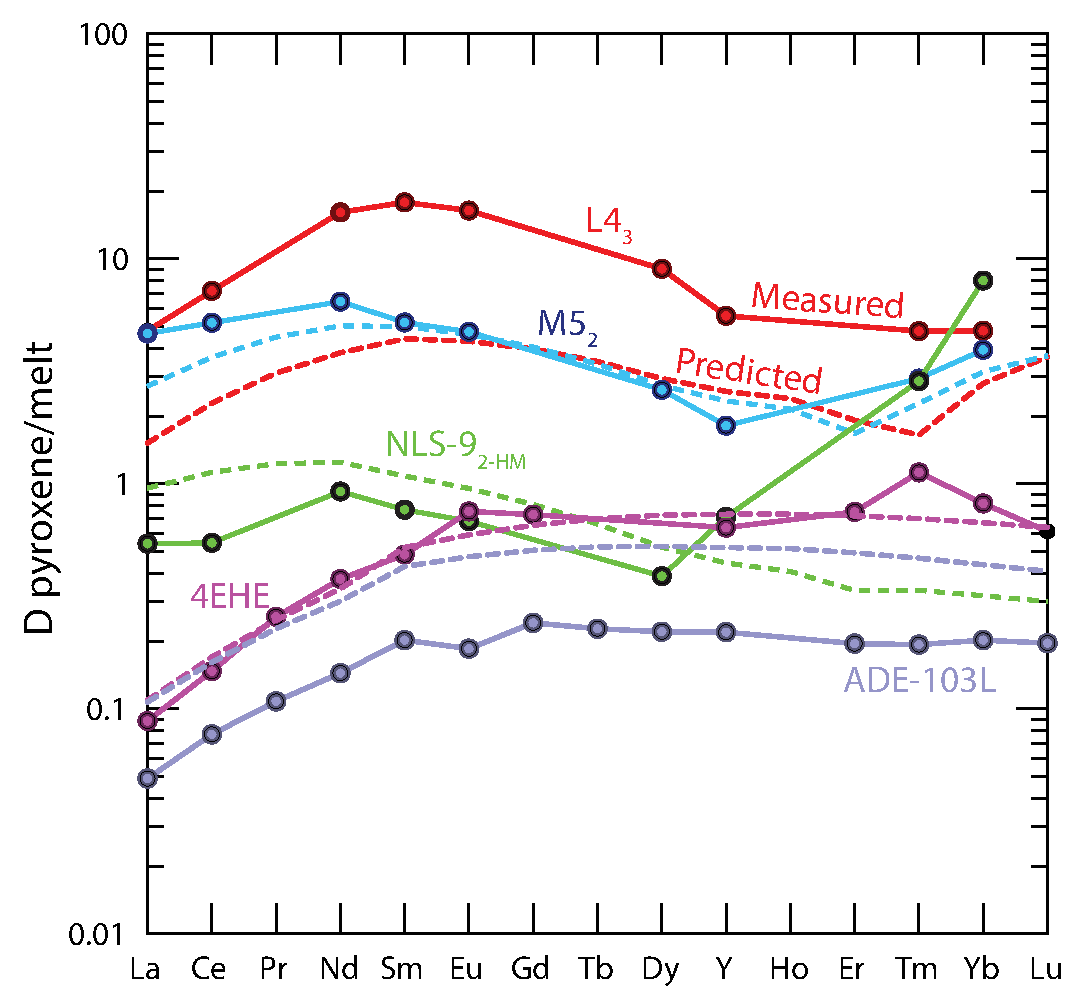
\includegraphics[width=0.45\textwidth]{14_SpiderDTest.eps}
        \caption[Measured (solid line) and predicted (dashed line) element-partitioning coefficients for \ce{R^{3+}}]{Measured and predicted element-partition coefficients for \ce{REE^{3+}}. The model does not introduce notable radius-dependent biases, except for in our high-aegirine clinopyroxene (NLS-9\ce{_{2-HM}} in green) for which $D_{HREE}$ are strongly underpredicted, owing to inaccurate return of $D_0^{M1}$. Shown for comparison are two diopside--melt pairs: 4EHE from \citet{Hill2000}, grown from a synthetic (NCMAS) basaltic andesite composition and ADE-103L from \citet{Lofgren2006} grown from a picritic composition based on the Angra dos Reis meteorite.}
        \label{14_REEradius}
        \end{center}
        \end{figure}

The model for $D_0^{M1}$ contains compositional terms from all three crystallographic sites in clinopyroxene. $X^T_{Al}$ has a strong positive correlation with $D_0^{M1}$, consistent with a charge compensation mechanism that aids incorporation of \ce{R^{3+}} cations, while terms for \ce{^{VI}M}1  and \ce{^{VIII}M}2 site cations may be indirectly recording melt compositional effects. Because $D_0^{M1}$ is unusually high for our high-aegirine experiments, they had to be excluded from the fitting procedure to permit model convergence. Therefore while the models for $r_0^{M1}$ and $E^{M1}$ are calibrated for use all the way to end-member aegirine the model for the $D_0^{M1}$ term is only calibrated for use up to $\sim$\ce{Ae_{50}}. Further experiments at conditions between those that generated our medium and high-aegirine clinopyroxene would be required to better constrain the clinopyroxene compositional record of $D_0^{M1}$ in strongly peralkaline Fe-rich magmas.

When applied to our experimental data, and the compilation of partition coefficients from Italian volcanoes \citep{Fedele2009, Mollo2013, Mollo2016}, the \ce{^{VI}M}1 stepwise model reproduces element-partitioning data to a factor of $\frac{+7}{-11}$ at the 95\% confidence interval (Fig. \ref{13_GlobalInv}b). Full regression reports are provided in \ref{Sup_RegressionReport}. 
% Mollo review: suggests bootstrapping model to determine the goodness of fit. See Putirka (2008) for procedure.


For convenience we provide an EXCEL spreadsheet for calculation of clinopyroxene-melt element-partition coefficients for any trace-element of 3+ valence that is large enough to fit onto the \ce{^{VI}M}1 or \ce{^{VIII}M}2 sites of clinopyroxene (\ref{EXCEL_D_Model}). 
	To assess the utility of the partitioning models and to monitor for potential introduction of radius-dependent bias, we show predicted REE patterns normalised to measured ratios for some literature data and our internally heated pressure vessel experiments (Fig. \ref{14_REEradius}). The model accurately reproduces REE patterns at all compositions, except for HREE on the \ce{^{VI}M}1 site of clinopyroxene at aegirine contents exceeding $\sim$50 mol \% (NLS experiments).

	%Fedele: Actually, also experiments L4 and ADE-103L did not produce a perfect matching between calculated and predicted Ds. The general measured patterns are well reproduced by predicted values, but the latter are systematically lower (L4) or higher (ADE-103L) with respect to the calculated values. I think it would be useful to add some comment (and possibly some explanation) about this in the text.
		                         
%----------------------------

\subsection{Implications for formation of REE deposits in evolved alkaline intrusions}
The solubility of REE and HFSE minerals is strongly enhanced in peralkaline melts \citep{Watson1979, Linnen1997, Boehnke2013, Aseri2015}, thus the high concentration of these elements in peralkaline systems may (partially) reflect this fact \citep{Dostal2017}. Melts containing high concentrations of REE and HFSE are thought to be generated through low degrees of partial melting in the mantle, followed by residual enrichment during protracted fractional crystallisation \citep{Marks2017}. The budget of REE and HFSE in a fractionating magma is influenced by the mineralogy of the crystallising assemblage, and the extent to which these elements are incorporated at minor or trace concentrations.

	Clinopyroxene is a major ferromagnesian phase that is commonly saturated throughout the entire differentiation histories of peralkaline magmatic systems \citep{Ablay1998,Marks2001a,Moller2016}. The composition of the fractionating clinopyroxene has a major impact on the absolute REE concentrations and REE pattern of the residual melt, and ultimately on the ability of a system to develop economic concentrations of the REE \citep[Fig. \ref{15_Fract_Cryst}, e.g.][]{Kogarko1990, Sorensen1992, Marks2011}.
Clinopyroxene in alkaline magmatic systems is initially calcic for mafic melts, and becomes increasingly sodic as crystal fractionation proceeds \citep{Marks2004}. Although the REE are compatible in the majority of our experimentally generated clinopyroxene, those approaching aegirine end-member composition, as found in evolved alkaline magmatic systems have the lowest $D_{REE}$ values (Fig. \ref{6_D_Spider}). Strongly alkaline magmatic systems are thought to crystallise abundant Ca-pyroxene early in their evolution which may deplete residual liquids with respect to REEs. Consequently, even though crystallisation of Na-pyroxene could enrich residual liquids with REE, the resultant concentration of these metals in the melt would remain low. 
    However, clinopyroxene is not the only phase to crystallise from alkaline magmas, and the majority of additional silicate phases, such as olivine, biotite and feldspar have $D_{REE} << 1$, typically 1-4 orders of magnitude lower than clinopyroxene \citep{Larsen1979,Kovalenko1988, Mahood1990,Fedele2015}.
    % Fedele: You can find partition coefficient data for plagioclase, alkali feldspar, biotite, magnetite and apatite in equilibrium with K-trachytic/phonolitic melts in Fedele et al. (2015, Am Mineral 100, 233-249), where  you can find also a compilation of literature data on such Ds for other evolved natural systems.
     Consequently, if the mode of clinopyroxene is low enough, the bulk $D_{REE}$ of the crystallising assemblage would remain below unity, allowing the REE to become enriched in the residual silicate melt.


%%%%%%%%%%%%%%%%%%%%%%%%%%%%%%%%
% Hypothetical stepwise fractional crystallisation in which the cpx compsition progressively changes

 \begin{figure}[bt]
        \begin{center}
        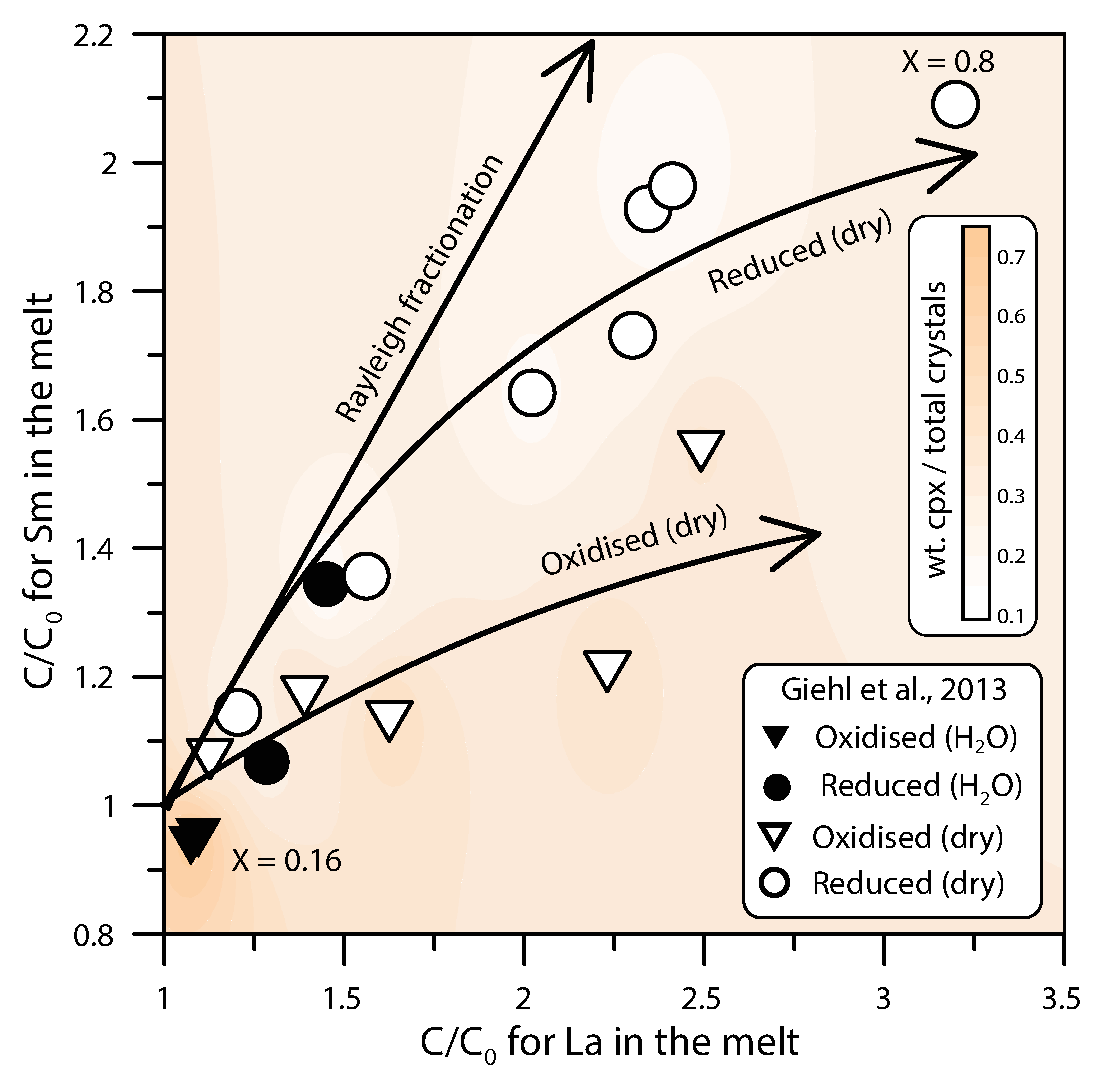
\includegraphics[width=0.45\textwidth]{15_FractCryst_Giehl_NoContours.eps}
        \caption[La vs. Sm diagram showing the geochemical evolution of the MiKa dyke, Gardar province, Greenland]    
        {Model enrichment paths for La and Sm in residual melts during fractional crystallisation of a MiKa dyke composition (Gardar Province, Greenland, see \citealt{Marks2003}). Phase relations and clinopyroxene compositions are from \citet{Giehl2013} and pertain to both oxidising and reducing conditions (log \fO = $\Delta$QFM -3 and +1), nominally dry to water bearing (to 3 wt.\% \ce{H2O} at 1 kbar). Colour shading indicates the weight fraction of clinopyroxene within the crystallising assemblage. Bold arrows indicate residual enrichment pathways for the REE in the melt for Rayleigh fractionation (no incorporation into crystals), reduced, dry conditions, and oxidised dry conditions (the latter two are hand drawn fits to the data). For simplicity, this model does not consider REE incorporation into magnetite, alkali-feldspar, olivine, nepheline or aenigmatite, all phases generated in the experiments of \citet{Giehl2013} \citep[see][]{Larsen1979,Kovalenko1988,Mahood1990}.}
        % \textbf{PLACEHOLDER from \citet{Mollo2016}.} Fractional crystallisation pathways showing the geochemical evolution of residual melts in equilibrium with clinopyroxene from alkaline magmatic systems. \emph{I would use clinopyroxene compositions from the MiKa dyke, Gardar Province, Greenland \citep{Marks2003}. There are rough estimate of temperature for these rocks that have allowed modelling of partition coefficients, but I have no handle on the degree of crystallisation between each clinopyroxene composition. I could arbitrarily choose values, but this does not feel satisfactory. \citet{Mollo2017} run a MELTS simulation, and \citet{Mollo2016} pictured in placeholder appear to choose values of fractionation arbitrarily. We cannot run a MELTS simulation, because our compositions are so far from the calibrated range of this model. Please advise: Any ideas on how I should choose fractionation factors?}}
        \label{15_Fract_Cryst}
        \end{center}
        \end{figure}

To give insight into the optimum conditions for residual magmatic enrichment of the REE in alkaline systems we modelled the evolution of REE concentrations in the melt during fractional crystallisation of a nepheline syenite body (Fig. \ref{15_Fract_Cryst}). Phase relation data and clinopyroxene compositions are from the experimental study of \citet[][]{Giehl2013}. Their starting composition, based on the MiKa dyke, from the Gardar Province, Greenland, is already extremely evolved, with Mg\# = 2, (Na + K)/Al = 1.44 and FeO* = 12 wt.\%.
% Rayleigh fractionation behaviour was modelled for all crystal phases, except for clinopyroxene (Afs, $\pm$ Mag, $\pm$ Ol, $\pm$ Nph, $\pm$ Ae). Bulk partition coefficients for the REE were calculated using major-element compositions for the clinopyroxene and the proportion of as part of the crystallising assemblage (calculations follow \citealt{White2013}).
		
		In these models, crystallisation under water-bearing, oxidising conditions produces a high fraction of clinopyroxene that depletes residual melts with respect to Sm, while subtly enriching La. 
	Dry conditions promote abundant alkali feldspar (Afs) crystallisation, which effectively enriches the REE content of residual melts. Under oxidising, dry conditions, the La/Sm ratio of the residual melt increases with fractionation, because Sm is more effectively incorporated into clinopyroxene.
Residual enrichment is most effective under dry, reducing conditions because of a relatively lower fraction of clinopyroxene within the crystallising assemblage. Because of this, the REE enrichment path of the residual melt is close to that of ideal Rayleigh fractionation.  
	Under these reducing, dry conditions and at a temperature of 750\dgCs, the experiments of \citet{Giehl2013} attained a crystal fraction of 0.8. Here, residual melts would have and 3.2 times La concentration and 2 times the Sm concentration relative to their starting composition. 

%Low pressure, dry conditions key for enrichment of REE: promotes crystallisation of Afs, a mineral that does not take significant REE into its structure. 

%Mollo review: Model a hypothetical stepwise F.C. pathway in which the cpx compositions progressively evolve from Ca- to Na- end-member. Check Fig 11 of Mollo et al., 2016 (Lithos?) and Fig. 12 of Mollo et al., 2017 (also Lithos).
% JS: This could perhaps be incorporated into your last section regarring the impact on alkaline melts and associated ore deposits. An example such as this wouldu be a useful addition.
% Discussion with JS and VvH: Use an F.C. pathway from the Marks/Markl group for this (MarksMarkl2003.

Considering these mechanisms, alongside our experimental and Canary Islands data, the best systems to develop high REE concentrations are those that would produce small proportions of Ca-pyroxene early in their crystallisation histories, quickly evolving to more sodic compositions that crystallise aegirine clinopyroxene. Cooling under low-pressure, dry, reducing conditions produces abundant alkali feldspar that in the case of a peralkaline composition, would serve to further increase the alkalinity of the residual melt.
	Low-degrees of source melting would produce primary melts with (1) high REE concentrations and (2) low melt Mg + Fe, and low modal abundance of clinopyroxene, which would aid enrichment in residual melts via fractional crystallisation.

% 	A slow-rifting tectonic environment may be important for REE mineralisation because in this setting, space is created in the crust into which low buoyancy, water poor low-degree melts can move. As these melts have low buoyancy, they would then stall in the `created space' in the crust, loosing heat slowly and undergoing extensive fractional crystallisation. 

% Slower cooling leads to lower TAl in the clinopyroxene, therefore lower REE contents \citep{Mollo2013}. And shallow, low pressure crystallisation is key to producing extensive quantities of alkali feldspar.

The HREE-rich nature of peralkaline magmatic systems, both granites and nepheline syenites, is compatible with fractionation of moderately sodic clinopyroxene that have high $D_{LREE}/D_{HREE}$ \citep[e.g.][]{Moller2016, Dostal2017}. As crystal fractionation progresses and clinopyroxene compositions evolve toward the aegirine end-member composition, $D_{LREE}/D_{HREE}$ decreases (Fig. \ref{6_D_Spider}). This systematic change in element-partitioning behaviour would result in strong HREE enrichment in aegirine-pyroxene cumulates, and would enrich the residual melt with respect to LREE-MREE.

%------------------------------------------

\section*{Conclusions}
\begin{itemize}
  \item Our experiments reveal three distinct element-partitioning behaviours for Na-rich clinopyroxene that depend on aegirine content. Each of these is associated with a distinct major-element exchange vector. We do not have the compositional resolution to know if the transition between these behaviours is smooth or step-like.
  
  \item Fits to the lattice-strain model of \citet{Blundy1994} indicate expansion of the \ce{^{VIII}M}2 site with increasing \ce{Na^+_{M2}}, to a maximum $r_{0, M2}^{3+}$ of 1.12 \si{\angstrom}{}  at \ce{Na^+_{M2}} = 0.4 c.f.u. Further expansion did not occur at higher Na contents.
  
  \item Both the \ce{^{VI}M}1 and \ce{^{VIII}M}2 sites of clinopyroxene shrink at high-aegirine contents in response to increasing $\sum$\ce{R^{3+}_{M1}}.
  
  \item Charge effects lead to a progressive increase in $D_0^{M1}$ at the expense of $D_0^{M2}$, as the exchanges \ce{Ca^{2+}} for \ce{Na+} and \ce{M^{2+}} for \ce{Fe^{3+}} take place. Much like in systems of lower alkalinity, REE incorporation into clinopyroxene is dominated by coupled Al--Si substitutions at the \ce{^{IV}T} site.
  
  \item Existing predictive models for clinopyroxene/melt element-partitioning do not accurately reproduce the large \ce{^{VIII}M}2 site ($r_{0, M2}^{3+}$) of our Na-rich clinopyroxene. We have calibrated a new empirical model that may be applied to any composition between basalt and peralkaline phonolite, based on our data from experiments and natural systems, as well as a large compilation of partition coefficients from the literature.
  
  \item Crystallisation of abundant Ca-Mg rich clinopyroxene depletes the residual melts of REE, and inhibits or terminates orthomagmatic enrichment processes.

  \item Clinopyroxene--melt REE partitioning systematics suggest that nepheline syenites which host REE deposits must originate from low-degree melts with sufficient alkali enrichment to saturate clinopyroxene similar to our medium-aegirine clinopyroxene (\ce{Ae_{25-50}}). Fractionation of such clinopyroxene enriches residual melts with respect to the HREE, in accord with the composition of REE-mineralised nepheline syenite systems.
  
  \end{itemize}

%------------------------------------------

\section*{Acknowledgements} 
We thank the Geo.X partners GFZ and Universit\"at Potsdam for access to the HP-GeoMatS Lab, Don Baker for assistance with preparation of starting materials, Bruce Watson and Volker M\"oller for providing samples of Mud Tank zircon and the Nechalacho Layered Suite rocks, respectively, Hans Peter Nabein, Maria Stuff and Julia Pohlenz for assistance with HP experimental equipment, Toby Soutar for help with preparation of the Canary Islands samples, Lang Shi and Glenn Poirier for assistance with electron-microprobe analyses, and Anna Jung for assistance with laser ICP-MS analyses. The manuscript benefited from discussions with Longbo Yang, Rebecca Paisley, Stephan Kolzenburg, Shane Rooyakkers and Jean B\'edard. Silvio Mollo, Lorenzo Fedele and an anonymous reviewer are thanked for their insightful feedback. Nelson Eby is thanked for editorial handling.
	This work was funded by PhD scholarships to C.B. from Geotop, DIVEX, and the SEG Canada Foundation, and operating grants to V.vH. and J.S. from the Natural Sciences and Engineering Research Council of Canada (grant numbers RGPIN-2014-05955, RGPAS-462335-2014) and the FQRNT team research project program.% (GRANT NUMBER TO INSERT).
 
%% References with bibTeX database:
\section*{References}
%\bibliographystyle{decsci}
\bibliographystyle{model2-names_NoURL}
\bibliography{library}

%% Authors are advised to submit their bibtex database files. They are
%% requested to list a bibtex style file in the manuscript if they do
%% not want to use model2-names.bst.


%%%%%%%%%%%%%%%%%%%%%%%%%%%%%%%%%%%%%%%%%%%%%%%%%%%%%%%%%%%%%%%%%%%%%
%%%%%%%%%%%%%%%%%%%%%%%%%%%%%%%%%%%%%%%%%%%%%%%%%%%%%%%%%%%%%%%%%%%%%
%%%%%%%%%%%%%%%%%%%%%%%%%%%%%%%%%%%%%%%%%%%%%%%%%%%%%%%%%%%%%%%%%%%%%
%%%%%%%%%%%%%%%%%%%%%%%%
\clearpage
\onecolumn
%\begin{singlespace}
\section{Tables}

\begin{table}[htpb]
\centering
\caption[Major-element composition of starting materials for the internally heated pressure vessel experiments.]{Major-element composition (in wt\%) of starting materials for the internally heated pressure vessel experiments. The totals are calculated with all iron as FeO.} %in excel 
\label{T_StMatTbl}
\begin{adjustbox}{max width=\textwidth}
\begin{tabular}{lllllllllll}
\toprule \multicolumn{11}{l}{\emph{Dry starting glass compositions calculated from masses of reagents added {[}wt\%{]}}}  \\
Composition   & \ce{SiO2}     & \ce{TiO2}      & \ce{Al2O3}    & FeOT     & MgO       & CaO      & \ce{Na2O}     & \ce{K2O}    & Total & (Na+K)/Al \\ \midrule
L4            & 57.48  & 1.50    & 19.00  & 5.89   & 1.61    & 3.21   & 7.33   & 3.98   & 100.00       & 0.861     \\
L5            & 61.24  & 0.68    & 19.51  & 3.77   & 0.43    & 0.91   & 8.63   & 4.84   & 100.00       & 0.996     \\
M3            & 52.67  & 2.27    & 18.13  & 7.86   & 2.75    & 5.40   & 7.19   & 3.73   & 100.00       & 0.875     \\
M4            & 56.35  & 1.47    & 18.63  & 5.77   & 1.58    & 3.15   & 8.48   & 4.57   & 100.00       & 1.014     \\
M5            & 60.04  & 0.66    & 19.13  & 3.69   & 0.42    & 0.89   & 9.76   & 5.41   & 100.00       & 1.145     \\
H4            & 54.80  & 1.43    & 18.12  & 5.62   & 1.54    & 3.06   & 10.07  & 5.38   & 100.00       & 1.236     \\
H5            & 58.38  & 0.65    & 18.60  & 3.59   & 0.41    & 0.86   & 11.31  & 6.20   & 100.00       & 1.362     \\
              &        &         &        &        &         &        &        &        &              &           \\
\multicolumn{11}{l}{\emph{Water saturated glass compositions from superliquidus experiments (EPMA) {[}wt\%{]}}}           \\ \midrule
L5            & 57.46  & 0.643   & 16.59  & 2.363  & 0.404   & 0.985  & 7.840  & 4.462  & 90.75  & 1.069  \\
s.d. (n = 8)  & 0.299  & 0.087   & 0.210  & 0.059  & 0.035   & 0.050  & 0.175  & 0.132  & 0.351  & 0.017  \\
rsd           & 0.52\% & 13.58\% & 1.26\% & 2.51\% & 8.70\%  & 5.09\% & 2.23\% & 2.97\% & 0.39\% & 1.57\% \\
              &        &         &        &        &         &        &        &        &        &        \\
H5            & 55.58  & 0.612   & 16.21  & 2.568  & 0.422   & 0.906  & 10.77  & 5.732  & 92.80  & 1.476  \\
s.d. (n = 13) & 0.327  & 0.057   & 0.221  & 0.113  & 0.044   & 0.049  & 0.205  & 0.154  & 0.417  & 0.028  \\
rsd           & 0.59\% & 9.33\%  & 1.36\% & 4.41\% & 10.44\% & 5.40\% & 1.90\% & 2.69\% & 0.45\% & 1.87\%  \\ \midrule

\end{tabular}
\end{adjustbox}
\end{table}

%%%%%%%%%%%%

 \begin{table}[htpb]
\caption{Summary of run conditions and run products for the internally-heated pressure vessel experiments.} 
\begin{adjustbox}{max width=\textwidth}
\begin{tabular}{lllllllll}
\toprule            &                 &           & \multicolumn{2}{l}{Cooling ramp} &           &             & Time         &          \\
Experiment   & Setup           & Pressure  & Rate         & Cycle & TE-1/TE-3 & TE-2 (spls) & (after ramp) & Run products         \\
             &                 & {[}bar{]} & \dgC/min       & +10\dgC & {[}\dgC{]}  & {[}\dgC{]}    & {[}h,m{]}     &                      \\ \midrule
L$4_3$        & IHPV RQ (f) 	   & 2038      & 1            & Y     & 825       & 828         & 44h50m       & Cpx + Ox + Ttn + Melt \\
L$5_3$        & IHPV RQ (f)     & 2038      & 1            & Y     & 825       & 828         & 44h50m       & Cpx + Ox + Melt       \\
M$3_2$        & IHPV RQ        & 2020      & 1            & Y     & 796/795   & 799         & 47h         & Cpx + Ox + Bt + Melt  \\
M$4_4$        & IHPV RQ        & 2020      & 1            & Y     & 796/795   & 799         & 47h         & Cpx + Ox + Bt + Melt  \\
             &                 &           &              &       &           &             &              &                      \\
M5           & IHPV            & 2000      & -            & -     & 800       & 799         & 47h55m       & Cpx + Bt + Fsp + Melt \\
M$5_2$     & IHPV RQ        & 2000      & -            & -     & 700       & 689         & 45h45m       & Cpx + Bt + Fsp + Melt \\
H$4_2$     & IHPV            & 2000      & -            & -     & 800       & 799         & 47h55m       & Cpx + Ttn + Melt      \\
H$5_2$     & IHPV RQ        & 2000      & -            & -     & 700       & 689         & 45h45m       & Cpx + Bt + Fsp + Melt \\
H$5_3$        & IHPV RQ        & 2020      & -            & -     & 651/649   & 648         & 46h15m       & Cpx + Bt + Fsp + Melt \\
             &                 &           &              &       &           &             &              &                      \\
NLS-9        & IHPV RQ        & 2020      & 1            & Y     & 651/649   & 648         & 46h15m       & Cpx + Ox + Melt       \\
NLS-$9_2HM$ & IHPV RQ**      & 2000      & 1            & Y     & 650       & 655         & 42h         & Cpx + Ox + Fsp + Melt \\ \midrule
\end{tabular}
\end{adjustbox}
\small{(f) indicates failure of the rapid quench apparatus; ** indicates use of a haematite double capsule, for run conditions at the haematite-magnetite \fO buffer \citep{Eugster1962}. Cpx = clinopyroxene; Ox = spinel oxide; Ttn = titanite; Bt = biotite; Fsp = sanidine feldspar.}  
\label{T_Exrun}  
\end{table}

 
		\begin{table}[htpb]
\caption{Representative major-element compositions of clinopyroxene and melt for the performed internally
heated pressure vessel experiments and Canary Islands phenocryst--glass pairs.}
%Fedele: How can you state these are representative compositions? As said in a previous comment, I have noticed that there actually is some compositional variability in both cpx nad glass from each run. Also, I cannot find any of these analyses in the Tables S1. Are these average values? This is getting confusing.
%I think it would be useful to report which of these belong to the low-, middle- or high-aegirine groupings presented in the text (or maybe just adding the aegirine molecula content).
\begin{adjustbox}{max width=\textwidth}
\begin{tabular}{@{}lllllllllll@{}}
\toprule
\emph{Pyroxene}  & L$4_3$ & M$3_2$ & M$5_2$ & H$5_3$ & NLS-9 & NLS-$9_2HM$ & \begin{tabular}[c]{@{}l@{}}16-07\\ LMB\end{tabular} & \begin{tabular}[c]{@{}l@{}}17-12\\ M. Samara\end{tabular} & \begin{tabular}[c]{@{}l@{}}17-14\\ UMB-II\end{tabular} & \begin{tabular}[c]{@{}l@{}}21-30\\ PV 2 ka\end{tabular} \\ \midrule
\ce{SiO2}      & 44.70 & 40.73 & 47.31 & 46.95 & 50.73 & 51.90       & 52.43                                                    & 51.77                                                           & 51.81                                                        & 52.50                                                                \\
\ce{TiO2}      & 3.07  & 4.57  & 3.17  & 4.47  & 0.10  & 0.10        & 0.80                                                     & 0.78                                                            & 0.74                                                         & 0.75                                                                 \\
\ce{Al2O3}     & 5.23  & 9.26  & 3.08  & 3.10  & 2.46  & 2.96        & 1.33                                                     & 1.24                                                            & 1.27                                                         & 1.22                                                                 \\
FeO       & 13.31 & 11.72 & 18.84 & 16.95 & 28.14 & 28.61       & 9.71                                                     & 9.62                                                            & 10.51                                                        & 10.02                                                                \\
MnO       & 0.01  & 0.01  & 0.01  & 0.00  & 0.25  & 0.17        & 0.78                                                     & 0.84                                                            & 0.91                                                         & 0.81                                                                 \\
MgO       & 9.09  & 9.28  & 5.55  & 6.05  & 0.05  & 0.07        & 12.30                                                    & 12.64                                                           & 12.07                                                        & 11.88                                                                \\
CaO       & 19.49 & 22.17 & 16.11 & 15.29 & 5.88  & 3.14        & 21.90                                                    & 21.76                                                           & 21.52                                                        & 22.02                                                                \\
\ce{Na2O}      & 2.27  & 1.01  & 4.34  & 4.97  & 9.86  & 11.45       & 1.18                                                     & 1.17                                                            & 1.38                                                         & 1.19                                                                 \\
\ce{K2O}       & 0.09  & 0.03  & 0.08  & 0.07  & 0.04  & 0.04        & 0.02                                                     & 0.03                                                            & 0.00                                                         & 0.02                                                                 \\
Total     & 97.25 & 98.78 & 98.49 & 97.85 & 97.49 & 98.45       & 100.44                                                   & 99.85                                                           & 100.22                                                       & 100.42                                                               \\
\emph{Glass}     &       &       &       &       &       &             &                                                          &                                                                 &                                                              &                                                                      \\ 
\ce{SiO2}      & 58.79 & 57.29 & 57.45 & 54.91 & 58.17 & 58.14       & 60.38                                                    & 55.10                                                           & 59.08                                                        & 60.04                                                                \\
\ce{TiO2}      & 0.35  & 0.27  & 0.23  & 0.62  & 0.00  & 0.00        & 0.64                                                     & 1.73                                                            & 0.66                                                         & 0.66                                                                 \\
\ce{Al2O3}     & 17.35 & 19.14 & 16.69 & 16.06 & 18.55 & 19.41       & 19.96                                                    & 18.30                                                           & 19.68                                                        & 19.79                                                                \\
\ce{Fe2O3}(T)  & 2.35  & 1.35  & 1.01  & 3.16  & 1.67  & 1.91        & 3.65                                                     & 7.22                                                            & 4.02                                                         & 3.96                                                                 \\
FeO(T)    & 2.12  & 1.22  & 0.91  & 2.84  & 1.50  & 1.72        & 3.28                                                     & 6.49                                                            & 3.62                                                         & 3.56                                                                 \\
MnO       & 0.02  & 0.00  & -     & 0.01  & 0.06  & 0.04        & 0.14                                                     & 0.23                                                            & 0.22                                                         & 0.20                                                                 \\
MgO       & 0.20  & 0.13  & 0.15  & 0.35  & 0.00  & 0.00        & 0.39                                                     & 1.84                                                            & 0.32                                                         & 0.35                                                                 \\
CaO       & 0.55  & 0.95  & 0.24  & 0.84  & 0.23  & 0.23        & 0.76                                                     & 4.10                                                            & 0.77                                                         & 0.74                                                                 \\
\ce{Na2O}      & 7.17  & 7.32  & 9.08  & 8.88  & 11.12 & 9.80        & 9.00                                                     & 7.26                                                            & 9.76                                                         & 9.05                                                                 \\
\ce{K2O}       & 4.68  & 4.10  & 4.68  & 5.30  & 1.51  & 2.51        & 5.41                                                     & 4.09                                                            & 5.45                                                         & 5.57                                                                 \\
Total     & 91.23 & 90.41 & 89.43 & 89.81 & 91.15 & 91.85       & 99.95                                                    & 99.13                                                           & 99.56                                                        & 99.95                                                                \\
(Na+K)/Al & 0.97  & 0.86  & 1.15  & 1.27  & 1.07  & 0.97        & 1.01                                                     & 1.12                                                            & 1.09                                                         & 1.09 \\ \midrule                                                           
\end{tabular}
\end{adjustbox}
\label{PxTbl}  
\end{table}

\begin{table}[htpb]
\centering
\caption{Pyroxene-melt trace-element-partition coefficients for representative experiments and a natural phenocryst-glass pair.}
\label{D_table}
\begin{adjustbox}{max width=\textwidth}
\begin{tabular}{@{}lllllllllllllll@{}}
\toprule
-  & L$4_3$  &        & M$3_2$  &        & M$5_2$  &        & H$5_3$  &        & NLS-9  &        & \multicolumn{2}{l}{NLS-$9_2 HM$} & \multicolumn{2}{l}{16-07-px4 LMB} \\ 
   & D      & $\sigma$      & D      & $\sigma$      & D      & $\sigma$      & D      & $\sigma$      & D      & $\sigma$      & D              & $\sigma$              & D                & $\sigma$               \\ \midrule
Li & 0.250  & 0.016  & 0.126  & 0.009  & 0.419  & 0.034  & 0.427  & 0.024  & 0.274  & 0.029  & 0.251          & 0.025          & 0.157            & 0.021           \\
Ga & 0.364  & 0.022  & 0.567  & 0.020  & 0.190  & 0.022  & -      & -      & -      & -      & -              & -              & 0.216            & 0.020           \\
Rb & 0.005  & 0.002  & 0.018  & 0.003  & 0.010  & 0.006  & 0.013  & 0.002  & 0.026  & 0.015  & -              & -              & 0.000            & 0.000           \\
Sr & 0.828  & 0.045  & 0.282  & 0.024  & 1.433  & 0.111  & 0.997  & 0.091  & 0.321  & 0.045  & 0.269          & 0.111          & 0.732            & 0.293           \\
Y  & 5.577  & 0.302  & 13.784 & 1.949  & 1.814  & 0.236  & 1.102  & 0.060  & 0.482  & 0.048  & 0.713          & 0.070          & 2.183            & 0.232           \\
Zr & 1.699  & 0.082  & 2.537  & 0.222  & 1.361  & 0.089  & 1.164  & 0.083  & 2.102  & 0.196  & 3.895          & 0.482          & 0.434            & 0.047           \\
Nb & 0.126  & 0.085  & 0.889  & 0.258  & 0.554  & 0.280  & 1.688  & 0.196  & 2.382  & 0.294  & 9.642          & 4.015          & 0.0062           & 0.0004          \\
Cs & 0.019  & 0.003  & 0.019  & 0.003  & 0.014  & 0.006  & 0.010  & 0.002  & -      & -      & 0.023          & 0.017          & 0.001            & 0.001           \\
Ba & 0.0364 & 0.0087 & 0.0373 & 0.0152 & 0.0388 & 0.0261 & 0.0288 & 0.0091 & -      & -      & -              & -              & 0.00004          & 0.00004         \\
La & 4.787  & 0.646  & 2.591  & 0.240  & 4.658  & 0.962  & 3.049  & 0.132  & 0.410  & 0.037  & 0.542          & 0.043          & 0.769            & 0.071           \\
Ce & 7.199  & 0.756  & 6.229  & 0.646  & 5.199  & 1.073  & 3.190  & 0.129  & 0.377  & 0.028  & 0.547          & 0.061          & 1.591            & 0.120           \\
Nd & 16.105 & 1.537  & 28.430 & 4.210  & 6.454  & 1.630  & 3.759  & 0.147  & 0.579  & 0.054  & 0.925          & 0.114          & 2.632            & 0.155           \\
Sm & 17.843 & 1.414  & 47.245 & 7.699  & 5.215  & 1.293  & 3.113  & 0.137  & 0.388  & 0.070  & 0.767          & 0.182          & 3.522            & 0.421           \\
Eu & 16.403 & 1.341  & 53.195 & 8.181  & 4.743  & 1.132  & 2.900  & 0.133  & 0.275  & 0.082  & 0.682          & 0.192          & 3.372            & 0.196           \\
Dy & 9.027  & 0.537  & 27.082 & 3.925  & 2.619  & 0.460  & 1.521  & 0.073  & 0.329  & 0.057  & 0.388          & 0.088          & 2.798            & 0.220           \\
Tm & 4.773  & 0.261  & 9.067  & 0.903  & 2.937  & 0.279  & 1.567  & 0.097  & 1.330  & 0.145  & 2.860          & 0.890          & 1.846            & 0.182           \\
Yb & 4.797  & 0.249  & 7.015  & 0.600  & 3.937  & 0.296  & 2.281  & 0.152  & 2.564  & 0.346  & 8.004          & 3.116          & 1.978            & 0.186           \\
Hf & 2.385  & 0.162  & 3.556  & 0.472  & 1.802  & 0.118  & 1.141  & 0.123  & 2.443  & 0.275  & 3.702          & 0.479          & 0.769            & 0.065           \\
Ta & 0.496  & 0.152  & 2.3694 & 0.6244 & 0.6502 & 0.2545 & 1.5654 & 0.2337 & 2.1082 & 0.1764 & 3.6854         & 0.6561         & 0.0153           & 0.0013          \\
Pb & 0.079  & 0.017  & 0.0587 & 0.0152 & 0.1142 & 0.0349 & 0.0199 & 0.0130 & 0.0884 & 0.0280 & 0.0564         & 0.0536         & 0.0203           & 0.0040          \\
Th & 0.201  & 0.034  & 0.3565 & 0.0419 & 0.3172 & 0.0321 & 0.2892 & 0.0239 & 0.0798 & 0.0240 & 0.0709         & 0.0276         & 0.0040           & 0.0003          \\
U  & -      & -      & 0.0512 & 0.0331 & 0.1261 & 0.0272 & 0.0196 & 0.0103 & 0.0460 & 0.0245 & 0.0834         & 0.0342         & 0.0022           & 0.0003          \\ \bottomrule
\end{tabular}
\end{adjustbox}
\end{table}



\begin{table}[]
\centering
\caption[Coefficients for prediction of lattice-strain parameters for clinopyroxene \ce{^{VI}M}1 and \ce{^{VIII}M}2 sites.]{Coefficients for prediction of lattice-strain parameters for clinopyroxene \ce{^{VI}M}1 and \ce{^{VIII}M}2 sites from clinopyroxene composition, temperature and pressure. Fitted vs. predicted lattice-strain parameters and partition coefficients are in Figures \ref{12_MLModel}--\ref{13_GlobalInv} and full multiple linear regression reports are available in \ref{Sup_RegressionReport}.}
\label{Coeff_Table}
\begin{adjustbox}{max width=0.7\textwidth}
\begin{tabular}{lllllll}
\toprule \multicolumn{3}{l}{Model for Ln$D_0$ \ce{^{VIII}M}2 site (n = 82)} &  & \multicolumn{3}{l}{Model for Ln$D_0$, \ce{^{VI}M}1 site (n = 16)} \\ 
 %                      &               &            &  &                   &                   &              \\
\emph{Parameter}              & \emph{Coefficient}   & $\sigma$    &  & \emph{Parameter}              & \emph{Coefficient}       & $\sigma$      \\ \midrule
Intercept              & 4.52          & 0.91       &  & Intercept         & 5                 & 1            \\
\ce{^{VI}M}1Ti                   & 6.8           & 3          &  & TAl               & 4                 & 0.5          \\
\ce{^{VI}M}1Al - \ce{^{VI}M}1\ce{Fe^{3+}}         & 1.6           & 0.6        &  & \ce{^{VI}M}1\ce{Fe^{2+}}            & 2.6               & 0.9          \\
\ce{^{VIII}M}2\ce{Fe^{2+}}                 & -3.8          & 1.3        &  & \ce{^{VIII}M}2Na              & -8                & 1            \\
T {[}K{]}              & -0.0035       & 0.0007     &  & \ce{^{VIII}M}2Ca              & -3                & 2            \\
TAl + T\ce{Fe^{3+}}           & 2.6           & 0.8        &  &                   &                   &              \\ 
$R^2$    &               & 0.647      &  &                   &                   & 0.959        \\
                       &               &            &  &                   &                   &              \\ \midrule
\multicolumn{3}{l}{Model for $E_s$, \ce{^{VIII}M}2 site (n = 79)}  &  & \multicolumn{3}{l}{Model for $E_s$, \ce{^{VI}M}1 site (n = 18)}   \\ 
%                       &               &            &  &                   &                   &              \\
\emph{Parameter}              & \emph{Coefficient}   & $\sigma$    &  & \emph{Parameter}              & \emph{Coefficient}       & $\sigma$      \\ \midrule
Intercept              & 247           & 44         &  & Intercept         & -2322             & 298          \\
\ce{^{VI}M}1Al                   & -424          & 144        &  & T {[}K{]}         & 3.2               & 0.4          \\
\ce{^{VI}M}1Mg                   & -285          & 102        &  & P {[}GPa{]}       & -408              & 145          \\
\ce{^{VI}M}1Ti                   & -1145         & 378        &  & \ce{^{VI}M}1Mg              & -800              & 212          \\
\ce{^{VIII}M}2Mg                   & -306          & 115        &  &                   &                   &              \\
P {[}GPa{]}            & 37            & 12         &  &                   &                   &              \\
TAl + T\ce{Fe^{3+}}           & 313           & 102        &  &                   &                   &              \\
XMg                    & 336           & 102        &  &                   &                   &              \\ 
$R^2$    &               & 0.348      &  &                   &                   & 0.936        \\
                       &               &            &  &                   &                   &              \\ \midrule
\multicolumn{3}{l}{Model for $r_0$, \ce{^{VIII}M}2 site (n = 82)}  &  & \multicolumn{3}{l}{Model for $r_0$, \ce{^{VI}M}1 site (n = 16)}   \\ 
%                       &               &            &  &                   &                   &              \\
\emph{Parameter}              & \emph{Coefficient}   & $\sigma$    &  & \emph{Parameter}              & \emph{Coefficient}       & $\sigma$      \\ \midrule
Intercept              & 1.01          & 0.02       &  & Intercept         & 0.79              & 0.03         \\
\ce{^{VI}M}1Ti                   & 0.16          & 0.05       &  & P {[}GPa{]}       & -0.017            & 0.005        \\
\ce{^{VI}M}1Al-\ce{^{VI}M}1\ce{Fe^{3+}}           & -0.03         & 0.01       &  & \ce{^{VIII}M}2Mg              & -0.48             & 0.06         \\
\ce{^{VIII}M}2Ca                   & 0.09          & 0.02       &  & \ce{^{VI}M}1\ce{Fe^{3+}}           & 0.14              & 0.03         \\
\ce{^{VIII}M}2Na                   & 0.14          & 0.02       &  & \ce{^{VIII}M}2Ca              & -0.05             & 0.02         \\
T {[}K{]}              & -4.46E-05     & 1.22E-05   &  &                   &                   & \\    
$R^2$    &               & 0.846      &  &                   &                   & 0.987         \\ \midrule        
\end{tabular}
\end{adjustbox}
\end{table}



 %%%%%%%%%%%%%%%%%%%%%%%%%%%%%%%%%%%%%%%%%%%%%%%%%%%%%%%%%%%%%%%%%%%%%
%%%%%%%%%%%%%%%%%%%%%%%%%%%%%%%%%%%%%%%%%%%%%%%%%%%%%%%%%%%%%%%%%%%%%
%%%%%%%%%%%%%%%%%%%%%%%%%%%%%%%%%%%%%%%%%%%%%%%%%%%%%%%%%%%%%%%%%%%%%



%%%%%%%%%%%%%%%%%%%%%%%%%%%%%%%%%%%%%%%%%%%%%%%%%%%%%%%%%%%%%%%%%%%%%
%%%%%%%%%%%%%%%%%%%%%%%%%%%%%%%%%%%%%%%%%%%%%%%%%%%%%%%%%%%%%%%%%%%%%
%%%%%%%%%%%%%%%%%%%%%%%%%%%%%%%%%%%%%%%%%%%%%%%%%%%%%%%%%%%%%%%%%%%%%
%%%%%%%%%%%%%%%%%%%%%%%%
%
%\FloatBarrier
%
%
%\section*{Figures}
\clearpage
\beginsupplement
\section{Supplementary figures}
% 
\begin{figure}[htpb]
\begin{center}
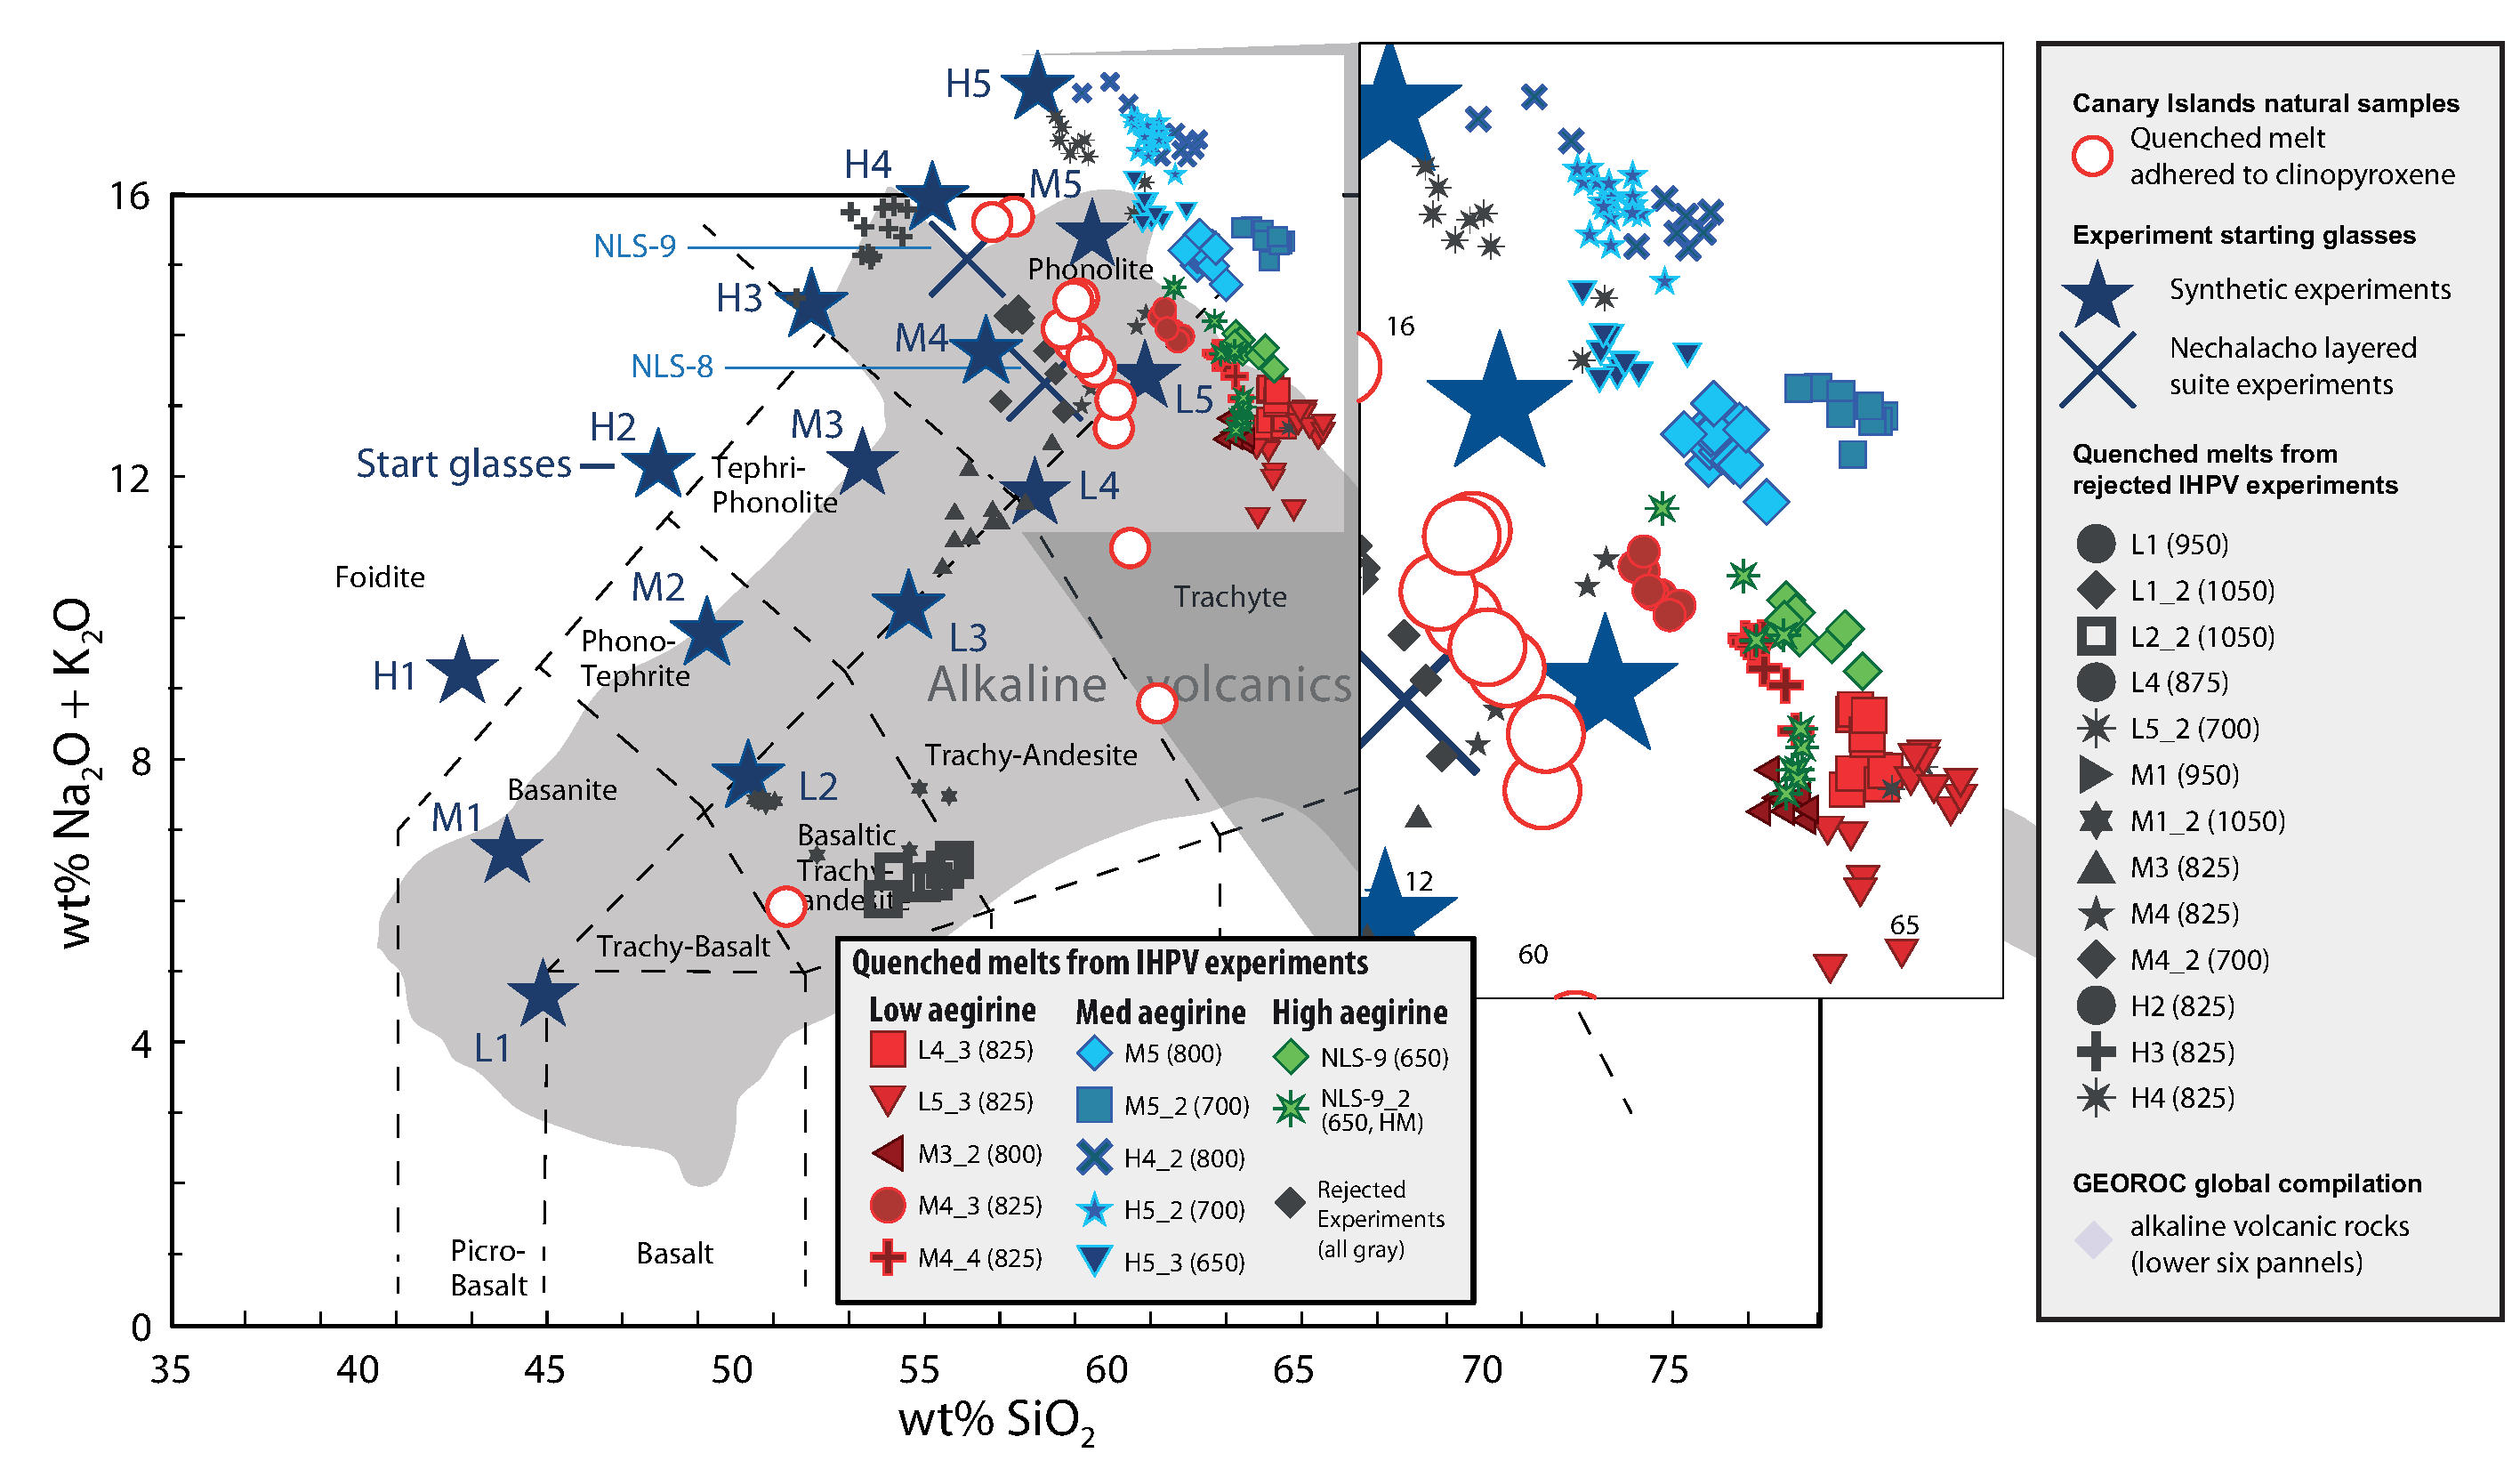
\includegraphics[width=1\textwidth]{S1_TAS_Aug2018.eps}
\caption[Total alkalies vs. silica diagram for glasses produced in the internally heated pressure vessel experiments]{Total alkalies vs. silica diagram for glasses produced in internally heated pressure vessel experiments and adhered to Canary Islands clinopyroxene phenocrysts \citep{LeBas1986TAS}. Large stars indicate synthetic starting glass compositions as used in internally heated pressure vessel experiments (Table \ref{T_StMatTbl}), whereas large crosses indicate the composition of powered natural samples from the Nechalacho layered suite, NT, Canada that were used as starting materials for some experiments. The gray field indicates the compositional range expressed by alkaline volcanic provinces from around the world, sourced from the GEOROC database. Rejected experiments in dark gray are not discussed in the main text, and either did not produce clinopyroxene, produced crystals that were too small for analysis by LA-ICP-MS, or grew crystals during quench, hence preserving disequilibrium partitioning behaviour. Further diagrams showing major-element compositions for the quenched melts and the starting glasses are in Fig \ref{S2_glass}.}
\label{TAS}
\end{center}
\end{figure}
% % Fedele: Glass data seems more homogenous, but in any case, in order to facilitate the comparison, in Table S1 I would more clearly separate the data for each different run (e.g., adding a column for the run lable or separating data for different runs using a blank row). Also, I would make a clearer separation of chosen and rejected data. All this can be done also for clinopyroxene data. 
% In any case, as remarked above for the cpx data, I don't think it is easy for the reader to make an idea about data homogeneity only looking at the Table S1, which is literally full of data. So, once more, I  think some additional figure could help a lot, and I think that compositional ranges should be discussed a little bit more in the text.

\begin{sidewaysfigure}[htp]
\begin{center}
\includegraphics[width=0.9\textwidth %, angle =90
]{S1_Glass_maj_Aug2018.eps}
\caption{Major-element compositions for glass produced in the internally heated pressure vessel experiments and adhered to clinopyroxene phenocrysts from the Canary Islands. Symbols as in Fig. \ref{TAS}.}
\label{S2_glass}
\end{center}
\end{sidewaysfigure}


%\begin{landscape}
\begin{sidewaysfigure}[htp]
\begin{center}
\includegraphics[width=0.9\textwidth %, angle =90
]{S2_Nov2016_maps_2-11-2016.pdf}
\caption[Element maps of clinopyroxene from internally heated pressure vessel experiments]{Element maps of clinopyroxene from internally heated pressure vessel experiments. M5 clinopyroxene have a sharp internal boundary that reflects feldspar saturation and are subtly zoned. NLS-9 clinopyroxene are more strongly zoned with swallowtail and hopper textures and rare inclusions of magnetite \citep[cf.][]{Walker1976, Lofgren1989,Shea2013}. H4 clinopyroxene (Px) display a bimodal crystal size distribution and occur with titanite (Ttn). The bimodal crystal size distribution is due to a temperature perturbation during run, and renders this experiment unsuitable for this element-partitioning study.}
\label{ElementMap_Supplement}
\end{center}
\end{sidewaysfigure}
%\end{landscape}

%\begin{SCfigure}
%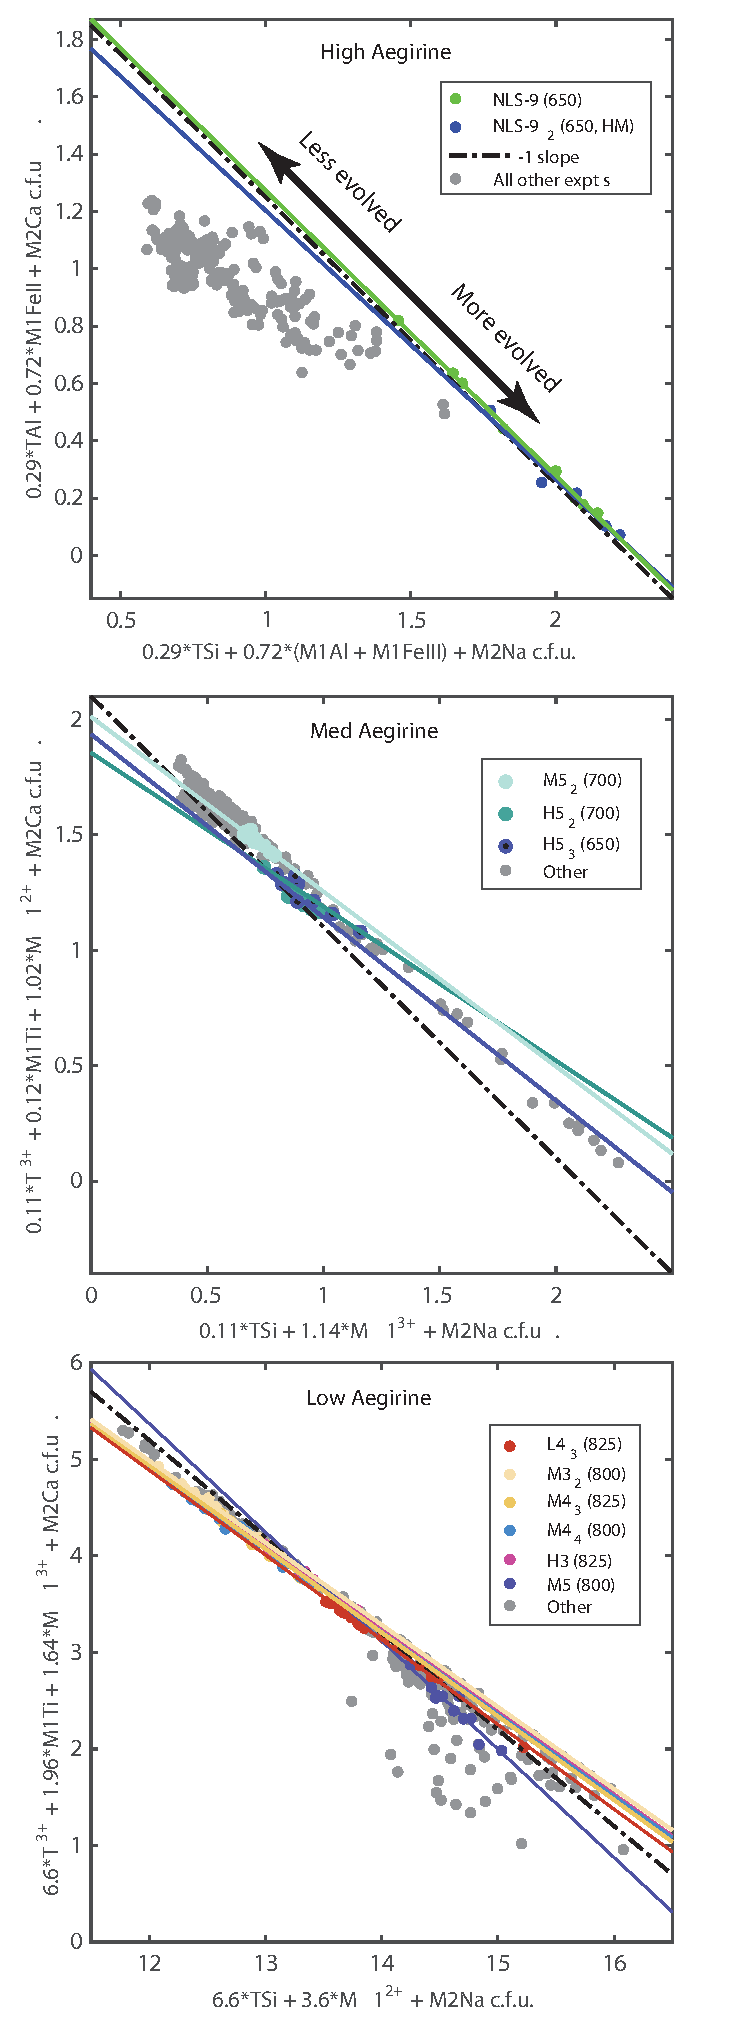
\includegraphics[width=0.4\textwidth]{S3_ExchMech_Feb2017-02.eps}
%\caption[Major-element exchange mechanisms]{Major-element exchange mechanisms for (a) high, (b) medium and (c) low-aegirine clinopyroxene generated in internally heated pressure vessel experiments. Each individual plotted point represents an electron-microprobe analysis. Axes were defined by linear regressions between site assigned element abundances, which have been checked for consistency in total site occupancy and charge.}
%\label{SF_ExchMech}
%\end{SCfigure}

        \begin{figure}[htpb]
\begin{center}
  \begin{minipage}[c]{.47\linewidth}
  \null
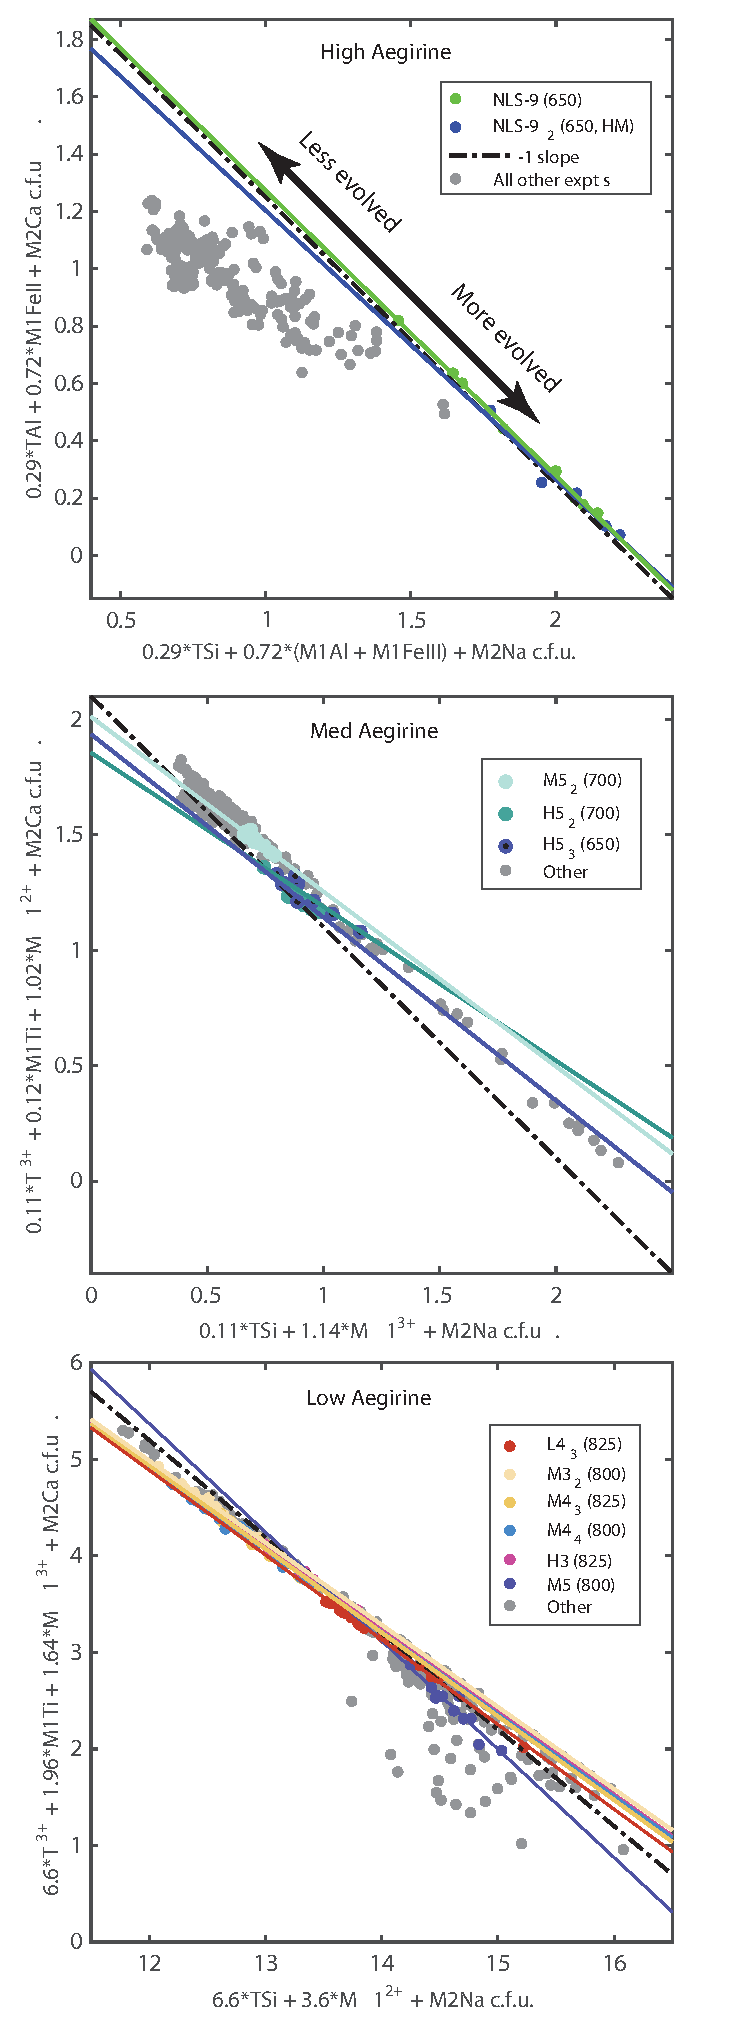
\includegraphics[width=1\textwidth]{S3_ExchMech_Feb2017-02.eps}
\end{minipage}\hfill
\begin{minipage}[c]{0.47\textwidth}
\caption[Major-element exchange mechanisms]{Major-element exchange mechanisms for (a) high, (b) medium and (c) low-aegirine clinopyroxene generated in internally heated pressure vessel experiments. Each individual plotted point represents an electron-microprobe analysis. Iron in the clinopyroxene was assigned to 2+ or 3+ valence following \citet{Droop1987}, then major-element cations were assigned to sites following \citet[][see \ref{EXCEL_D_Model}]{Morimoto1989}. Axes were defined by linear regressions between site-assigned major-element abundances, which have been checked for consistency in total site-occupancy and for charge.}
\label{SF_ExchMech}
\end{minipage}
\end{center}
\end{figure}


\begin{figure}[htp]
\begin{center}
\includegraphics[width=0.7\textwidth]{S5_D_XNaM2}
\caption[Element partition coefficients for HFSE (Ti, Zr, Nb), REE (La, Sm, Yb) and TE (Li, Th) vs. $X^{M2}_{Na}$]{Element partitioning coefficients for HFSE (Ti, Zr, Nb), REE (La, Sm, Yb) and TE (Li, Th) vs. $X^{M2}_{Na}$. Literature values (n = 411), including those from Italian volcanoes, are from the compilation of \citet{Bedard2014}.}
\label{D_XM2Na}
\end{center}
\end{figure}

%%%%%%%%%%%%%%%%%
\clearpage

\appendix

\section{Electronic appendix of chemical data (.xlsx)}
\label{Ae_SupTbl} 
Electronic appendix (.xlsx file) containing experiment starting glass compositions, experiment run conditions, mineral abundances in experimental charges, compositions of reference materials used for EPMA and LA-ICP analyses, major-element concentrations for experiment glasses and clinopyroxene, partition coefficients and fitted lattice-strain parameters.

%   \begin{table}[htpb]
% \centering
%  \begin{tabular}{c}
% xlsx
%     \end{tabular}
% \caption[Electronic appendix of chemical data (.xlsx)]{Electronic appendix (.xlsx file) containing experiment starting glass compositions, experiment run conditions, mineral abundances in experimental charges, compositions of reference materials used for EPMA and LA-ICP analyses, major-element concentrations for experiment glasses and clinopyroxene, partition coefficients and fitted lattice-strain parameters.}
% \label{Ae_SupTbl} 
% \end{table}

\section{Locations for the Canary Islands samples (.kml)} \label{Waypoints}  Electronic appendix (.kml file) containing field locations for the Canary Islands samples.


%   \begin{table}[htpb]
% \centering
%  \begin{tabular}{c}
% kml
%     \end{tabular}
% \caption[Field locations for Canary Islands samples (.kml)]{Electronic appendix (.kml file) containing field locations for the Canary Islands samples.}
% \end{table}
\section{The Laser Ablation ICP-MS unmixing model}
\label{LaserMix}

\begin{figure}[htb]
\begin{center}
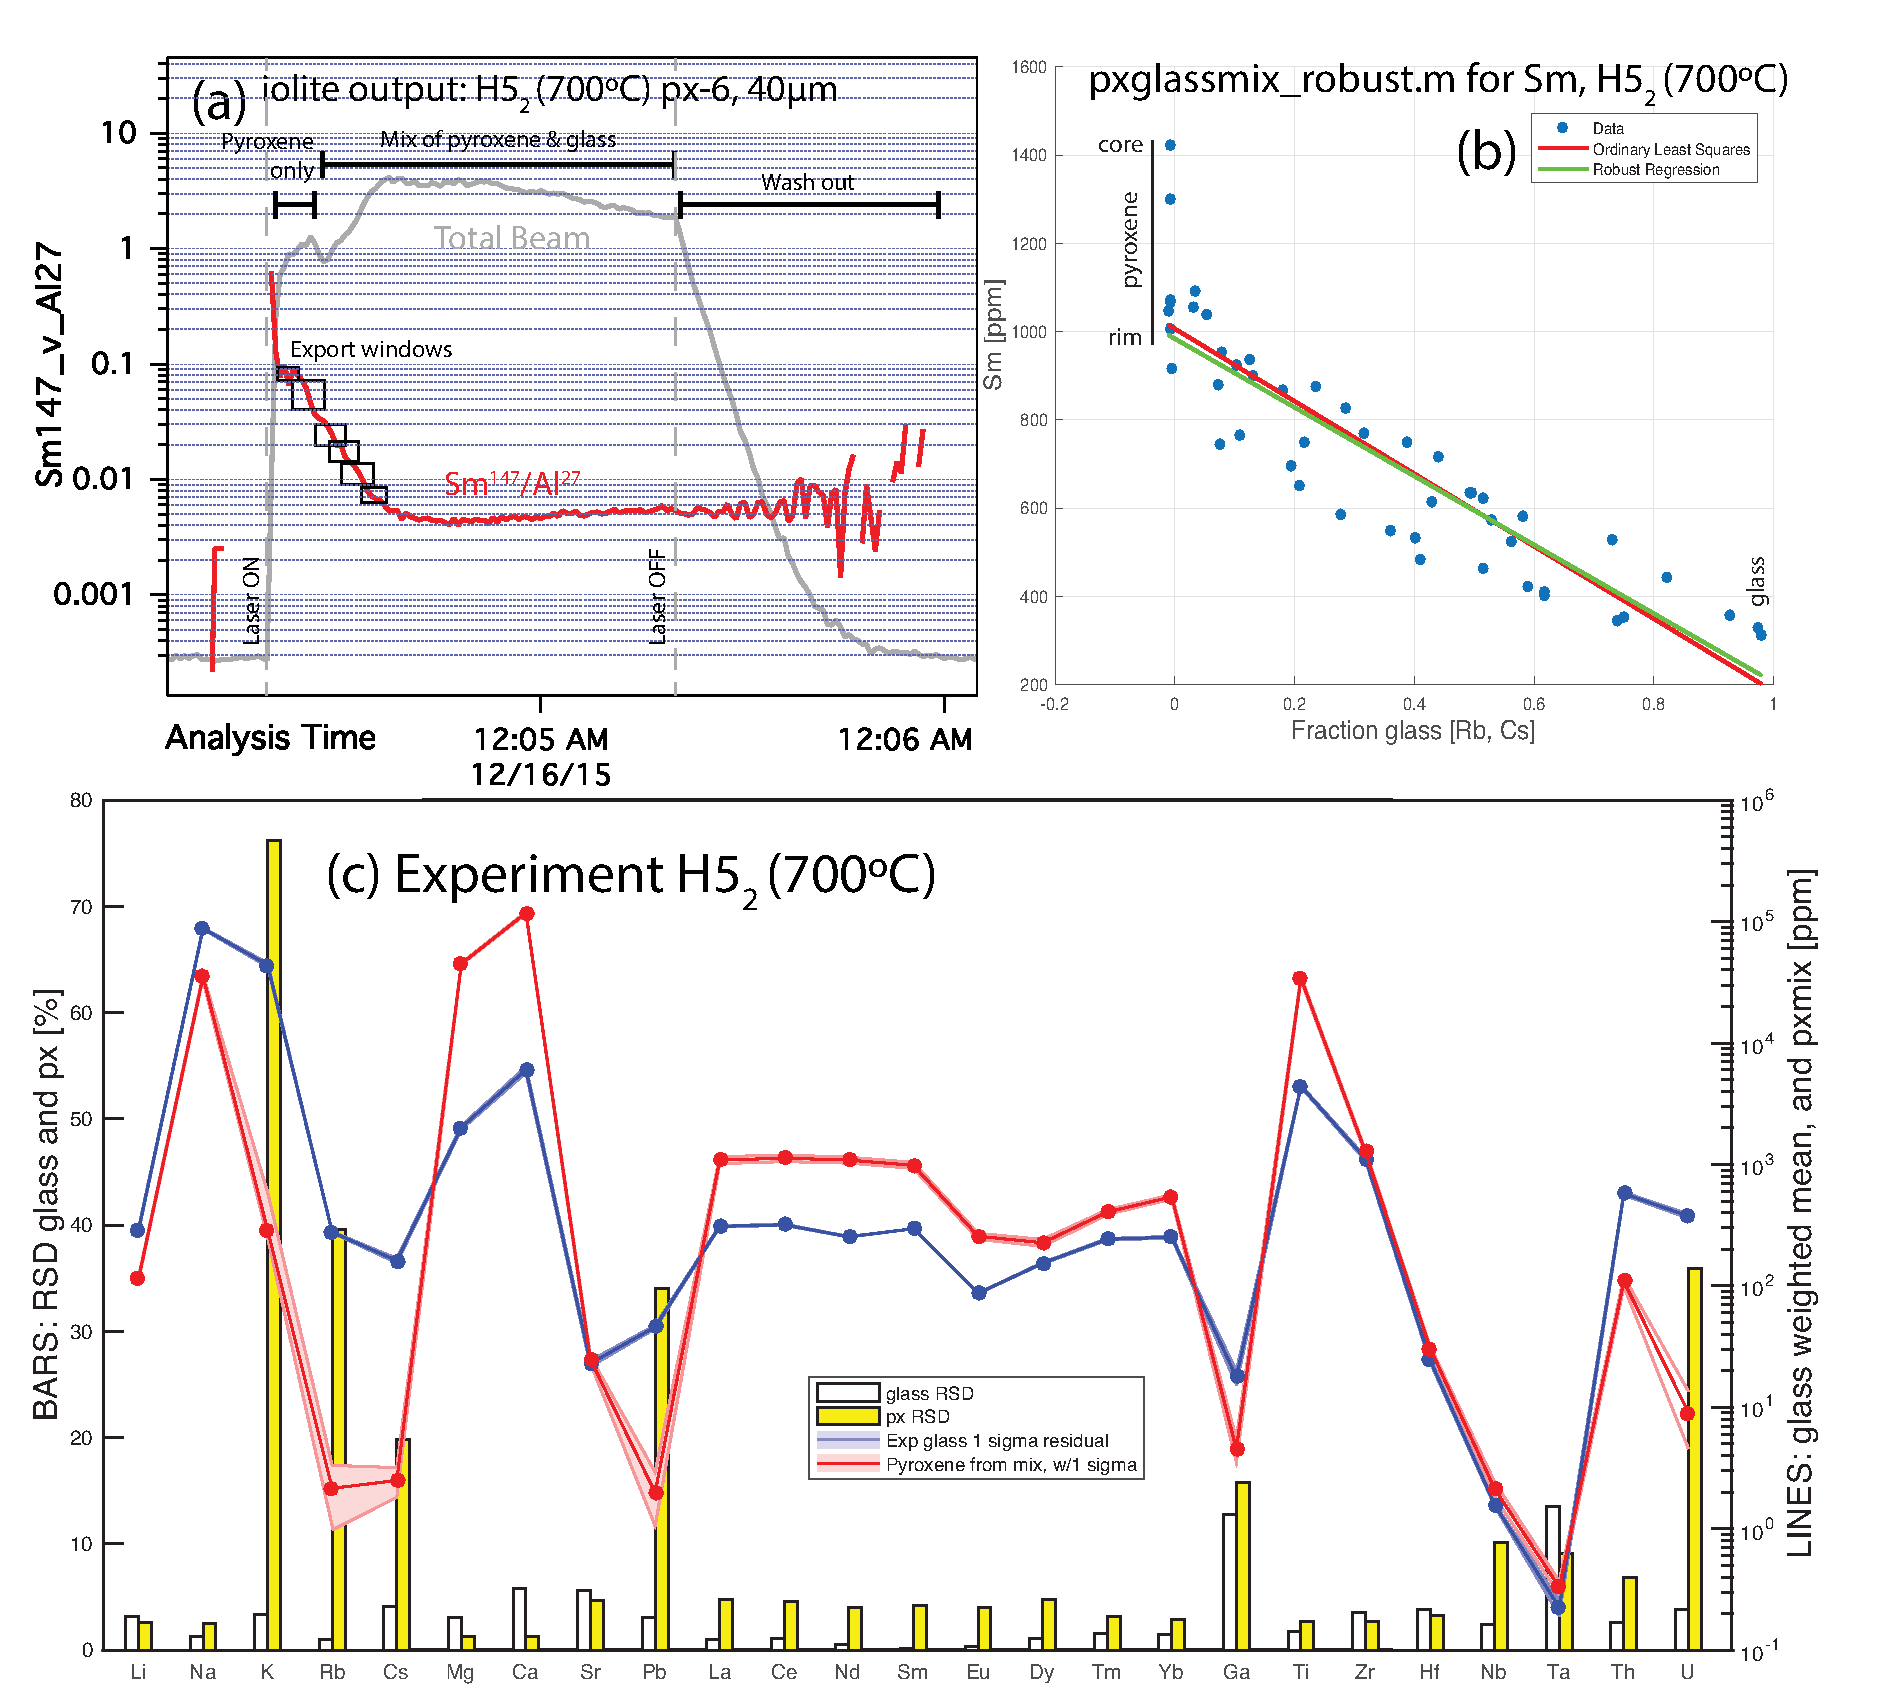
\includegraphics[width=0.85\textwidth]{S4_QAQC_LaserMix_H5_2}
\caption[An example of the robust regression data reduction scheme for laser-ablation ICP-MS analyses of glass and clinopyroxene mixtures.]
    {An example of the robust regression data reduction scheme for laser-ablation ICP-MS analyses of glass and clinopyroxene mixtures. (a) Time series of laser-ablation data as displayed in by the iolite v2.5 extension for Igor Pro \citep{Paton2011}, (b) a MATLAB output diagram from the robust regression unmixing script, and (c) a quality control diagram output from the same MATLAB script. %This data reduction methodology returns trace-element concentrations in clinopyroxene that are within analytical uncertainty of those derived via regular time-integrated data reduction methods.
    }
    \label{LaserMixFig}
\end{center}
\end{figure}

The LA-ICP-MS robust regression data reduction scheme described here allows for determination of mineral trace-element compositions where the grains of interest are smaller than the laser spot-size. The mathematics underpinning the script are similar those of \citet{Rubatto2007} and from our research group, of \citet{Yang2018}. 
Assumptions include...

		whilst effectively rejecting outlier data, for example from the ablation of minerals other than clinopyroxene that may have been hidden below the polished surfaces of the grain mounts




Initially, the raw counts-per-second data are imported into Igor Pro, running the iolite v2.5 extension \citep{Paton2011} where drift and background corrections are made. Mixed signals of clinopyroxene show characteristic stepped peaks in element-ratio and beam intensity traces (Figure \ref{LaserMixFig}a). Outputs are exported in short time windows as shown.

Trace-element concentrations in the mixes are then normalised to the sum of major-element oxides, as measured by LA-ICP-MS.

TO COMPLETE


(a) Time series of laser-ablation data, showing traces for Sm/Al (red) and total beam intensity (gray). The laser beam often ablated through the small clinopyroxene crystals, returning a mixed signal that was exported from the iolite data reduction software in short time windows as shown. Data were then normalised to the sum of major-element concentrations and mixes were deconvolved using a robust regression script written in MATLAB. (b) An example output diagram for the robust regression data reduction scheme. Clinopyroxene--glass mixing ratios were constrained by strongly incompatible elements Rb and Cs. For each element, a robust linear regression was defined between the fraction of glass in the mixture and element concentration. The intercept of this regression with zero glass returned the trace-element concentrations in the clinopyroxene. Uncertainty with this technique is typically below 10 \% relative (median 9.3 \% at the 1$\sigma$ level). In this example, the Sm-rich core of a zoned clinopyroxene crystal is effectively rejected during data processing, and the derived Sm concentration for the clinopyroxene is therefore closer to that of the clinopyroxene rims that are in equilibrium with the adjacent quenched melt. (c) A quality control diagram output from the MATLAB data reduction scheme showing the concentrations of various elements in the glass and clinopyroxene (lines) and the uncertainty on these concentrations expressed as a relative standard deviation (bars). Derived partition coefficients ($D_i$) are the mass concentration of element \emph{`i'} in clinopyroxene divided by that in the adjacent quenched melt. Residuals for the $D_i$ values were calculated using uncertainties derived from the clinopyroxene and glass analyses to calculate minimum and maximum partition coefficients at the 1$\sigma$ level. These are reported in Table \ref{D_table} and \ref{Ae_SupTbl}


\section{EPMA Ce concentration transects across experiment clinopyroxene (.xlsx)} \label{CeTransects}  

Electronic appendix (.xlsx file) containing electron-microprobe transects across experiment clinopyroxene for Ce, Mg and Fe. The data indicate that $D_{Ce}^{px/melt}$ values determined from our experiments are overestimates, but only by up to 25\%. Sector zoning in the clinopyroxene appears to have a larger impact on apparent Ce partitioning behaviour than growth zoning.

% \begin{table}[htpb]
% \centering
%  \begin{tabular}{c}
% xlsx
%     \end{tabular}
% \caption[Ce concentration transects across experiment clinopyroxene (.xlsx)]{Electronic appendix (.xlsx file) containing electron-microprobe transects across experiment clinopyroxene for Ce, Mg and Fe. The data indicate that $D_{Ce}^{px/melt}$ values determined from our experiments are overestimates, but only by up to 25\%. Sector zoning in the clinopyroxene appears to have a larger impact on apparent Ce partitioning behaviour than growth zoning.}
% \label{CeTransects}  
% \end{table}

    
\section{Multiple linear regression reports (.pdf)}
\label{Sup_RegressionReport}

Electronic appendix (.pdf file) containing multiple linear regression reports from the stepwise fitting of 3+ cation lattice-strain parameters for the predictive model for element-partitioning (39 pages).


\section{Numerical model for prediction of clinopyroxene/melt element-partitioning coefficients for ions of 3+ valence (.xlsx)} 
\label{EXCEL_D_Model}

Electronic appendix (.xlsx file) containing a numerical model for prediction of clinopyroxene/melt element-partitioning coefficients for ions of 3+ valence. Required input data are major-element oxide compositions for clinopyroxene, pressure and temperature. The model for the \ce{^{VIII}M}2 site is calibrated for application to systems of basaltic to peralkaline phonolite composition. The model for the \ce{^{VI}M}1 site is calibrated for use on alkaline to weakly peralkaline systems where the aegirine mol\% in clinopyroxene does not exceed 50.

%supplement: Chemical heterogeneity and the approach to equilibrium during the experiments
\section{Supplement: Chemical heterogeneity and the approach to equilibrium during the experiments}
\label{ApproachEq_Sup}
\subsection{Attainment of equilibrium in the Canary Islands rocks}
The Canary Islands trace-element partition-coefficients presented here were determined from euhedral, blade-shaped crystals free of melt inclusions and chemical zonation. The corresponding quenched melt was in direct contact with these crystals and shows no zonation in backscattered electron images (Fig. \ref{3_ChemTransect}). While equilibrium conditions are challenging to confirm for a natural volcanic system, the euhedral forms, chemical homogeneity of crystals, and congruency between samples from separate eruptions suggest that the crystals grew in a stable environment, and were not subject to chemical or physical perturbations during growth (Fig. \ref{6_D_Spider}).	

\subsection{Attainment of equilibrium in the experiments}
%See Adam1993 start of discussion. There is a long section entitled "Heterogeneity and approach to equilibrium during experiments"
Experiments used to determine trace-element partition-coefficients must have attained, or at least closely approached, chemical equilibrium. Unfortunately no experiments are able to determine equilibrium trace-element partition-coefficients \emph{sensu stricto} because reversal experiments, where a clinopyroxene re-equilibrates with a melt, are not possible owing to sluggish diffusion of most elements through the clinopyroxene structure \citep{VanOrman2001,Zhang2010}.
     The following two sections discuss some analytical and experimental biases that must be considered when determining mineral-melt trace-element partition-coefficients from crystallisation experiments.

%%%%%%%%%
%SEE REMOVED MATERIAL TEX
%%%%%%%%%
\subsubsection{The formation of diffusive boundary layers}
A potential barrier to chemical equilibration during crystallisation is the formation of a diffusive boundary layer within the melt adjacent to growing crystals. In a perfect equilibrium case there are no compositional gradients in the melt at any time during crystal growth. However in reality the growth of crystals depletes compatible elements from the melt and residually enriches incompatible elements. 
    Theoretically, this process of crystal growth results in formation of a (potentially ephemeral) diffusive boundary layer in the melt directly adjacent to the crystal that is depleted with respect to compatible elements and enriched with respect to those that are incompatible \citep{Lu1995}. The composition of such a diffusive boundary layer depends on both the relative enrichment or depletion of elements during the crystallisation process, and the rate at which these elements diffuse through the melt. Rapidly-diffusing elements with partition-coefficients close to unity will have concentrations closest to that of the bulk melt.

Experiments designed to investigate trace-element-partitioning behaviour might employ slow cooling rates to limit the development of diffusive boundary layers, thus forming crystals from melt that is closer in composition to that of the bulk experiment. Such experiments then run into another problem, in that significant crystallisation may occur at temperatures above that of the final run temperature. Rapidly-cooled experiments circumnavigate this issue, but may form relatively more pronounced diffusive boundary layers during crystal growth that become `flattened out' during the homogenisation stage of the experiment.

Numerous diffusion data have been gathered for silicate melts over the past few decades, and a comprehensive review is given by \citet{Zhang2010}. Diffusion of trace-elements through water-saturated peralkaline melts is rapid, owing to their depolymerised structure. For example Lanthanum diffusion-coefficients are 6 orders of magnitude higher than for water-saturated granitic compositions of a similar temperature \citep[compare][]{Rapp1986,Behrens2009}. This rapid diffusion serves to minimise the formation of diffusive boundary layers adjacent to growing crystals in our experiments.
Coupled diffusion mechanisms complicate the application of measured single-element diffusion-coefficients to a crystallising system \citep{Grove1984,Liang1994,Costa2003}. Here, the diffusive flux of trace-elements may be coupled to gradients in major-element concentration within the melt. 

%%%%%%%%%%%%%%%

To investigate the impact of diffusive effects on trace-element-partitioning between clinopyroxene and melt, \citet{Mollo2013} performed crystallisation experiments on trachybasaltic melts at a range of cooling rates (2.5--50\dgC/ hr). Rapid cooling rates result in depletions of Si, Ca and Mg in the clinopyroxene that are compensated for by enrichments in Al, Na and Ti. Regardless of cooling rate, Ounma parabolae could be fitted through isovalent sets of partition-coefficients, indicating that crystal-lattice-effects dominated over those associated with the formation of diffusive boundary layers and that local equilibrium was achieved at the time of crystallisation.
    % In their rapidly-cooled experiments, \citet{Mollo2013} found apparent clinopyroxene/melt trace-element-partition coefficients that varied systematically with the \ce{^{IV}Al} content of the clinopyroxene, regardless of cooling rate.
    In their rapidly-cooled experiments \citet{Mollo2013} found apparent clinopyroxene/melt trace-element partition-coefficients that varied with identical crystal-chemical systematics to true equilibrium partition coefficients, the magnitude of both sets of trace-element partition-coefficients following the \ce{^{IV}Al} content of the clinopyroxene (ibid., their Fig. 9). 
Deviations of the partition coefficient of several orders of magnitude can be obtained only when rapidly growing crystals entrap small portions of the diffusive boundary layer that are found as minute melt inclusions randomly distributed in the mineral phase \citep{Kennedy1993}. In this extreme case, partitioning behaviour is obviously influenced by contamination phenomena and no Onuma parabolae can be derived. As Onuma parabolae could successfully be fitted through partitioning data for all of our presented experiments (see following sections), and no melt inclusions were observed in optical and electron imaging, we infer that our data were not affected by the presence of such melt inclusions, and that they may be compared directly with partitioning data derived from experiments that employed slower cooling rates.

 %S. Mollo, email via Vincent 29Jan2018:
 %Also, the following point of the Reviewer2 is not entirely correct: "The presence of major-element concentration gradients around the natural crystals investigated leads me to expect even larger REE concentration gradients around the growing crystals. If this is true, the reported partition coefficients are minima and maxima rather than representative of equilibrium. In this case, the data are inappropriate for lattice-strain modeling, particularly as a part of a larger dataset comprising experiments at equilibrium". Reading through Mollo et al. (2013) published in CTMP, you will see that the lattice-strain modeling can be successfully applied under rapid growth conditions when a diffusive boundary layer develops at the crystal-melt interface. This implies that the "true" partition coefficient changes as an "apparent" partition coefficient. If the lattice-strain equation fits the Onuma diagram (i.e., partition coefficient versus ionic radius), it can be concluded that local equilibrium condition was attained at the time of crystallization. Moreover, apparent partition coefficients change by quantities of the same order of magnitude of the true partition coefficients due to crystallographic effects (Mollo et al., 2013). Deviations of the partition coefficient of several orders of magnitude can be obtained only when rapidly growing crystals may entrap small portions of the diffusive boundary layer that are found as minute melt inclusions randomly distributed in the mineral phase (Kennedy et al., 1993). But in this case the partition coefficient is obviously influenced by contamination phenomena and no Onuma parabolas can be derived.
 
 %% VvH email 29Jan2018: Also, a quick check of the Ce data from the probe shows that the max deviation between rim composition and grain average would be a factor of 1.5 (most are between 1.1 and 1.3). So this does not seem to be an issue at all. Lang unfortunately did not send me all the data, but I?ll gather the remainder on Tuesday. I doubt that the other data will change anything though. 
 
%%%%%%%%%


\subsubsection{Chemical zonation in the experiment clinopyroxene: Theoretical framework}
Trace-elements diffuse slowly through the clinopyroxene structure relative to that of the melt \citep{VanOrman2001, Zhang2010}, therefore no re-equilibration of trace-elements takes place on an experimental time scale. Strictly speaking, clinopyroxene only record true equilibrium conditions at their outermost rim. 
     Experiments designed for the derivation of equilibrium partition coefficients ideally minimise bias by limiting the fraction of crystallisation, producing minerals that are as homogeneous as possible. Currently available \textit{in situ} analytical techniques for trace-element abundances, such as LA-ICP-MS and SIMS, are limited in terms of minimum beam-size to $\sim$10 $\mu$m; chemical zonation, however subtle, will be continuous from the core to the rim of the mineral. Consequently, no experimentally-derived partition-coefficients record chemical equilibrium \textit{sensu stricto}, but properly conducted experiments may closely approximate this state.

Because only the very rim of a crystal records chemical equilibrium with the adjacent melt, and some internal portions of the minerals must be sampled during \textit{in-situ} analyses all experimentally-determined trace-element partition-coefficients are biased toward higher values for compatible elements and lower values for incompatible elements. The magnitude of these biases depends on the fraction of crystallisation in the experiment, the true equilibrium partition-coefficient of that element, as well as the proportion of each growth-zone sampled during the \textit{in-situ} analysis. Fortunately \textit{in-situ} chemical analyses preferentially sample the mantle and rim of zoned crystals because few analyses section a crystal perfectly through the core. As a result there is a sampling bias toward equilibrium mineral compositions.

	% % Fedele: You never talked about average values... [CB: comment addressed, removed.]

	Consider a hypothetical experimental system in which 20\% of the melt crystallises as a single mineral, and where the chemical analyses of that mineral are truly bulk averages of that mineral composition. An incompatible element with a true equilibrium partition coefficient of 0.1 would return a measured partition coefficient of 0.09, a small bias because the concentration of that incompatible element in the melt changed only subtly during the course of crystallisation. For compatible elements with true $D_i$ values of $\sim 10$, measured partition coefficients can be a factor of 2--3 higher than true partition coefficients, because their concentration in the melt changes more than an incompatible element during the course of crystallisation.

    Further complexity is introduced in systems that crystallise multiple minerals simultaneously. In the case of experiment M3\ce{_2}, the REE are compatible in clinopyroxene, but are incompatible in biotite and oxides \citep[e.g.][]{Mahood1990,Schmidt1999}. The REE have therefore been residually enriched in the melt phase by the crystallisation of biotite and oxide minerals, while simultaneously being depleted from the melt by crystallisation of clinopyroxene. These two competing processes serve to minimise the effect of fractional crystallisation on the concentration of trace-elements in the melt and consequently derived REE partition-coefficients between clinopyroxene and melt will be closer to true equilibrium values.

\subsubsection{Implications of the cerium zonation across the experiment clinopyroxene}
    Electron-microprobe analyses offer a smaller minimum beam-size than LA-ICP-MS systems at the expense of precision and of number of elements that may be analysed simultaneously. This higher spatial resolution permitted investigation of the zonation of Ce concentrations within the experiment clinopyroxene, with Ce as a proxy for the other compatible elements.

% As presented above, the effect of sector-zoning on the Ce concentration in the experiment clinopyroxene strongly outweighs that of concentric growth zoning. 

The magnitude of concentric growth zoning in the experiment clinopyroxene was examined by averaging bulk and rim compositions across multiple sector-zoned grains within each experiment. The median Ce counts divided by the rim Ce counts was 1.04 for experiment M3\ce{_2}, 1.08 for experiment M5 and 1.12 for the fluorine-bearing experiment M3-1.25F \citep[see][]{Beard_PhD_thesis}. Contrary to theory discussed above, the subtly (3\%) crystallised experiment M5 shows a greater variation in core-to-rim Ce content than the more heavily (?? TO ADD\%) crystallised experiment M3\ce{_2}. Furthermore, the $D_{Ce}^{cpx/melt}$ for experiment M3\ce{_2} (6.2) is approximately double that for experiment M5 (see discussion below), which should further promote the formation of Cerium zonation in the clinopyroxene during crystallisation. Consequently it is possible that many existing experimentally-derived trace-element partition-coefficients are systematically offset from true equilibrium values.

If Cerium is used as a proxy for the behaviour of compatible elements in our experimental system, then apparent partition coefficients derived for these elements via LA-ICP-MS are systematically offset to higher values by 4--8\%. Such a systematic bias is small, relative to the variation in clinopyroxene-melt partition coefficients within our sample set, as well as in the literature. The effect of crystal zonation on incompatible element concentrations was not measured, but as outlined in the theoretical framework above, this effect should be smaller than that for the compatible elements. No correction factor has been applied to the data presented in the figures below, or in Table \ref{D_table} and \ref{Ae_SupTbl}. 

%%%%%%%%%%



\end{document}
%% End of file `elsarticle-template-2-harv.tex'.